\chapter{Phân tích hệ thống và thiết kế trang web}

\section{Nghiên cứu liên quan}

\subsection{LinkedIn}

LinkedIn là một mạng xã hội chuyên nghiệp hàng đầu thế giới, được thiết kế để kết nối với các cá nhân, doanh nghiệp và tổ chức trên toàn cầu. LinkedIn ra mắt vào năm 2003, được thiết kế để cung cấp nền tảng giúp người dùng xây dựng hồ sơ cá nhân chuyên nghiệp, mở rộng mối quan hệ nghề nghiệp, tìm kiếm cơ hội việc làm và chia sẻ kiến thức trong các lĩnh vực chuyên môn. LinkedIn không chỉ là nơi để bạn tạo dựng thương hiệu cá nhân mà còn là công cụ hữu ích để doanh nghiệp tìm kiếm nhân tài và phát triển mạng lưới kinh doanh.


\subsubsection{Ưu điểm của LinkedIn:}

\begin{itemize}
	\item \textbf{Mạng lưới kết nối rộng:} Do là một nền tảng lớn nhất thế giới dành riêng cho mục đích nghề nghiệp, nên LinkedIn có một mạng lưới kết nối rất lớn bao gồm nhiều quốc gia, ngôn ngữ khác nhau. Chính vì đó, LinkedIn giúp tạo cơ hội cho người dùng dễ dàng kết nối với các chuyên gia, nhà tuyển dụng hay các đối tác trên toàn thế giới.
	\item \textbf{Hỗ trợ tìm kiếm việc làm:} LinkedIn là một trong những công cụ tìm việc trực tuyến phổ biến nhất. Hàng ngàn công ty đăng tuyển trên nền tảng này, điều này giúp người dùng dễ dàng tìm kiếm cơ hội việc làm phù hợp.
	\item \textbf{Tham gia các nhóm chuyên môn:} LinkedIn có nhiều nhóm chuyên đề, cho phép người dùng có thể thảo luận, chia sẻ và học hỏi những kinh nghiệm và kiến thức từ những người dùng khác.
	\item \textbf{Xây dựng thương hiệu cá nhân:} LinkedIn chính là một bản CV trực tuyến, là nơi giúp người dùng trình bày kinh nghiệm, kỹ năng và thành tích của mình. Điều này giúp người dùng tự mình xây dựng thương hiệu cá nhân của riêng mình và thu hút sự chú ý của các nhà tuyển dụng.
	\item \textbf{Nội dung học hỏi và phát triển:} LinkedIn Learning cung cấp nguồn tài nguyên phong phú, bao gồm các bài viết, video và các khoá học trực tuyến về nhiều lĩnh vực khác nhau, giúp người dùng nâng cao kỹ năng và cập nhật xu hướng nghề nghiệp mới nhất.
\end{itemize}

\subsubsection{Hạn chế của LinkedIn:}

\begin{itemize}
	\item \textbf{Cạnh tranh cao:} Do là một nền tảng phổ biến cho tìm kiếm việc làm, nên lượng người dùng lớn và chuyên nghiệp. Điều này có thể làm giảm cơ hội của người dùng trong quá trình tìm kiếm công việc mong muốn và làm việc nổi bật trong lĩnh vực của bạn trên LinkedIn có thể gây khó khăn, đặc biệt nếu hồ sơ vẫn chưa được hoàn thiện hay tối ưu.
	\item \textbf{Vấn đề ngôn ngữ:} Vì là một nền tảng phổ biến nhất thế giới với mục đích tìm kiếm công việc, nên LinkedIn chủ yếu sử dụng tiếng anh làm ngôn ngữ chính. Điều này có thể gây khó khăn cho những người dùng không thông thạo tiếng anh. 
	\item \textbf{Khả năng tiếp cận:} Mặc dù là một nền tảng quốc tế với lượng người dùng khổng lồ thế nhưng LinkedIn chỉ phù hợp với những người tìm kiếm việc làm có tính chuyên nghiệp cao. Do đó, đối với các nhà tuyển dụng nhỏ lẻ ở Việt Nam, họ thường tập trung chủ yếu ở những trang tìm kiếm việc làm phổ biến ở trong nước.
	\item \textbf{Tập trung ở các ngành nhất định:} LinkedIn thường tập trung nhiều vào các ngành nghề có tính chất quốc tế như: công nghệ thông tin, tài chính và kinh doanh. Tuy nhiên, đối với các ngành nghề thủ công, nghệ thuật hoặc truyền thống, thường không được LinkedIn tập trung, để ý. 
\end{itemize}

\subsection{TopCV}

TopCV là một trang web, nền tảng tìm kiếm việc làm và tạo CV hàng đầu ở Việt Nam. TopCV được ra mắt vào năm 2016, nó đã trở thành lựa chọn đáng tin cậy cho hàng triệu người Việt Nam dùng trong việc xây dựng hồ sơ ứng tuyển chuyên nghiệp và tìm kiếm cơ hội việc làm phù hợp. Với giao diện thân thiện, dễ sử dụng và kho dữ liệu việc làm khổng lồ, TopCV đã trở thành cầu nối hiệu quả giữa các nhà tuyển dụng và người tìm việc.

\subsubsection{Ưu điểm của TopCV}

\begin{itemize}
	\item Công cụ tạo CV chuyên nghiệp: TopCV cung cấp nhiều mẫu CV hiện đại và dễ sử dụng, giúp người dùng tạo ra các bản CV ấn tượng một cách nhanh chóng và tiện lợi.
	\item Giao diện thân thiện, hỗ trợ tiếng việt: TopCV có giao diện đơn giản, thân thiện, dễ sử dụng và có hỗ trợ tiếng việt giúp người dùng  dễ sử dụng nếu không quen với giao diện quốc tế của nước ngoài.
	\item Hệ sinh thái đa dạng: Cung cấp việc làm từ nhiều ngành nghề khác nhau, đặc biệt phù hợp với thị trường lao động trong nước.
	\item Cộng đồng người dùng lớn: TopCV có một cộng đồng người dùng đông đảo, tạo ra nhiều cơ hội kết nối và trao đổi thông tin giữa người tìm việc và nhà tuyển dụng.
\end{itemize}


\subsubsection{Hạn chế của TopCV}

\begin{itemize}
	\item Mạng lưới kết nối: So với LinkedIn thì mạng lưới TopCV tập trung chủ yếu vào thị trường Việt Nam. Do đó, điều này phần nào hạn chế cơ hội tìm kiếm việc làm ở các quốc gia khác.
	\item Độ nhận diện thương hiệu quốc tế thấp: TopCV mặc dù được biết đến rộng rãi trong nước,thế nhưng trong thị trường quốc tế lại không có sức hút lớn với các nhà tuyển dụng.
	\item Nội dung chuyên sâu hạn chế: Trong khi LinkedIn cung cấp nhiều bài viết, thảo luận và khóa học chuyên sâu từ các chuyên gia hàng đầu, TopCV tập trung nhiều hơn vào tính năng tuyển dụng và tạo CV.
\end{itemize}


\subsection{Tổng kết}

Dưới đây là bảng so sánh các chức năng của 2 trang web với trang web của đồ án này - RabbitCV:

\begin{table}[H]
    \centering
    \begin{tabular}{|c|>{\centering\arraybackslash}p{0.07\linewidth}|>{\centering\arraybackslash}p{0.07\linewidth}|>{\centering\arraybackslash}p{0.07\linewidth}|>{\centering\arraybackslash}p{0.07\linewidth}|>{\centering\arraybackslash}p{0.07\linewidth}|>{\centering\arraybackslash}p{0.07\linewidth}|>{\centering\arraybackslash}p{0.07\linewidth}|>{\centering\arraybackslash}p{0.07\linewidth}|>{\centering\arraybackslash}p{0.07\linewidth}|} \hline 
         &  Tìm kiếm việc làm&  Đăng bài tuyển dụng&  Đăng tin tức&  Giao tiếp&  Chọn CV Template&  Chỉnh sửa CV&  Custom CV&  Bảng xếp hạng& Chia sẻ CV\\ \hline 
         LinkedIn&  \checkmark&  \checkmark&  \tikzxmark&  \checkmark&  \tikzxmark&  \tikzxmark&  \tikzxmark&  \tikzxmark& \checkmark\\ \hline 
         TopCV&  \checkmark&  \checkmark&  \checkmark&  \checkmark&  \checkmark&  \checkmark&  \tikzxmark&  \tikzxmark& \tikzxmark\\ \hline 
 RabbitCV& \checkmark& \checkmark& \checkmark& \checkmark& \checkmark& \checkmark& \checkmark& \checkmark&\checkmark\\ \hline
    \end{tabular}
    \caption{Bảng so sánh trang web với RabbitCV}
    \label{tab:related_works}
\end{table}



\section{Phân tích hệ thống}
\subsection{Stakeholder}

Stakeholder (hay còn gọi là các bên liên quan) là những cá nhân hoặc tổ chức có lợi ích hoặc ảnh hưởng đến một dự án, công ty hay tổ chức. Họ có thể bao gồm: các nhà đầu tư, khách hàng, nhân viên, nhà cung cấp, chính phủ,.... Mỗi nhóm stakeholder có thể có những mong đợi và yêu cầu khác nhau và việc quản lý mối quan hệ với họ là rất quan trọng để đảm bảo sự thành công của dự án hoặc công ty.

Trong dự án này, tôi phân loại các bên liên quan thành 2 phần: các bên liên quan chính (internal skateholder) và các bên liên quan thứ yếu (external skateholder). Các bên liên quan chính là những người có ảnh hưởng trực tiếp đến hệ thống hoặc dữ liệu. Còn các bên liên quan thứ yếu là những bên không có ảnh hưởng trực tiếp đến hệ thống hoặc dữ liệu, nhưng họ đóng vai trò quan trọng trong việc cung cấp dữ liệu và tuân thủ quy định của hệ thống.

\subparagraph{Các liên quan chính trong dự án của tôi:}
\begin{itemize}
    \item  \textbf{Admin:} là những người chịu trách nhiệm quản lý và duy trì hệ thống, cập nhật nội dung và hỗ trợ người dùng. Họ tương tác trực tiếp với hệ thống và có vai trò quan trọng trong việc đảm bảo hệ thống hoạt mạnh mẽ, mượt mà và hiệu quả. Họ chính là người duyệt các bài đăng tuyển dụng và tin tức, họ cũng là người sẽ cung cấp tài khoản, mật khẩu cho các công ty/doanh nghiệp nếu họ muốn tiếp cận trang web.
    \item \textbf{Người sử dụng/Người nộp đơn xin việc:} là những người sử dụng chính trong trang web. Họ là người sử dụng trang web để tạo, chỉnh sửa hoặc xoá CV, đồng thời, tìm kiếm công việc khi cần thiết. Họ có thể tìm kiếm các công việc và nộp đơn xin việc nếu công việc thực sự phù hợp với mình. Việc cập nhật hồ sơ cá nhân và kinh nghiệm việc làm thường xuyên góp phần giúp cho các nhà tuyển dụng hiểu được mình và tăng cơ hội được trúng tuyển. Và khi được ứng tuyển, họ có thể tương tác với các nhà tuyển dụng thông qua trang web.
    \item \textbf{Công ty/Doanh nghiệp:} Họ sẽ người chịu trách nhiệm trong việc đăng các tin tuyển dụng để tìm kiếm ứng viên phù hợp cho các vị trí công việc, đồng thời, họ cũng có thể viết các bài tin tức giới thiệu về công ty. Họ có thể theo dõi và quản lý các đơn xin việc đã nhận được trong việc sàng lọc, phỏng vấn và tuyển chọn ứng viên. Sau khi xác nhận các đơn xin việc của ứng viên, họ có thể giao tiếp với sinh viên thông qua trang web hoặc gmail.
\end{itemize}

\subsubsection{Các bên liên quan thứ yếu trong dự án của tôi:}
\begin{itemize}
    \item \textbf{Chính phủ:} chính là bên liên quan thứ yếu đầu tiên ở đây. Họ không ảnh hưởng trực tiếp đến hệ thống nhưng họ có thể ảnh hưởng đến hệ thống thông qua các quy định pháp luật liên quan đến tuyển dụng và bảo vệ dữ liệu người dùng.
    \item \textbf{Người dùng gián tiếp:} Họ là những người hưởng lợi từ dữ liệu mà không cần tương tác trực tiếp đến hệ thống.
    \item \textbf{Cộng đồng:} là nhân tố quan trọng góp phần cung cấp phản hồi về trải nghiệm sử dụng của trang web giúp cải thiện các tính năng và dịch vụ. Việc xây dựng một cộng đồng lớn cũng giúp tạo uy tín cho trang web và lan rộng, phổ biến trang web cho nhiều người hơn, từ đó, có tiền để đầu tư và phát triển trang web hơn.
\end{itemize}

\subsection{Các yêu cầu của hệ thống}

\subsubsection{Các yêu cầu chức năng}

\begin{enumerate}
    \item Tự thiết kế CV cho chính mình hoặc chọn các template CV theo ý mình
    \item Chia sẻ CV ra cho những nhà tuyển dụng xem xét.
    \item Xuất file CV thành pdf
    \item Thêm, xoá, sửa và xem CV
    \item Tìm kiếm công việc trong danh sách tuyển dụng.
    \item Tạo nhóm/nhắn tin giữa nhà tuyển dụng và người dùng.
    \item Nhà tuyển dụng có thể đăng tuyển tuyển dụng.
    \item Chức năng đăng nhập với 3 vai trò: admin, user, recruiter
    \item Có thể sao lưu, ưa thích công việc phù hợp với mình hoặc các CV mà mình hứng thú.
\end{enumerate}
 

\subsubsection{Các yêu cầu phi chức năng}


\begin{enumerate}
    \item Duy trì hoạt động trang web 24/7
    \item Hỗ trợ hình ảnh, ký tự đặc biệt vào CV.
    \item Giao diện dễ nhìn, dễ sử dụng
    \item Dữ liệu hệ thống được tổ chức sao cho dễ dàng cho việc bảo dưỡng, bảo trì và nâng cấp. Khi hệ thống gặp lỗi, đảm bảo thời gian sửa chữa và bảo trì hệ thống trở lại bình thường là 3 tiếng.
    \item Khi thay đổi hệ thống, dữ liệu được đảm bảo lưu giữ và chuyển giao đầy đủ đến hệ thống mới.
    \item Có thể tạo nhiều CV với nhiều templates khác nhau.
    \item Tốc độ tải trang trang nhanh chóng.
    \item Đảm bảo bảo mật thông tin của khách hàng, xác thực tài khoản mỗi khi đăng nhập.
    \item Trang web có khả năng xử lý nhiều người dùng mà không bị gián đoạn hay chậm đi.
    \item Có khả năng xử lý lượng truy cập cao đặc biệt ở các giờ cao điểm.
\end{enumerate}

 \section{Lược đồ usecase (Usecase diagram)}
 \subsection{Thiết kế lược đồ usecase}
 
\subsubsection{Lược đồ usecase chung}

\begin{figure}[H]
	\centering
    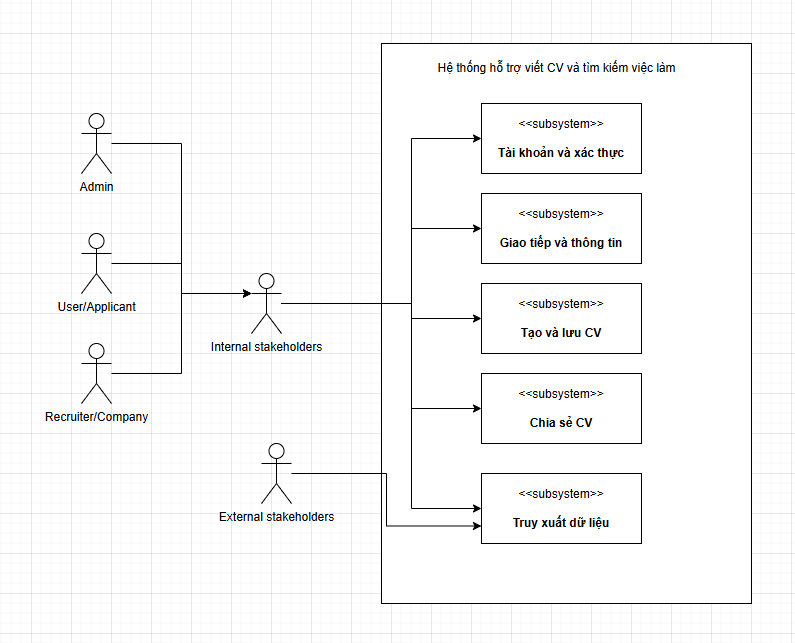
\includegraphics[scale = 0.6]{img/general_usecase.png}
    \caption{Lược đồ usecase chung}
\end{figure}

Hệ thống của trang web hỗ trợ viết CV và tìm kiếm việc làm sẽ chia làm 3 hệ thống nhỏ bao gồm:
\begin{itemize}
    \item \textbf{Hệ thống tài khoản và xác thực:} Thành phần này đảm nhận nhiệm vụ giám sát các tài khoản và xử lý các quy trình xác thực tài khoản.
    \item \textbf{Hệ thống giao tiếp và quản lý thông tin:} Thành phần này chịu trách nhiệm quản lý các tin nhắn và các thông tin của người dùng, CV.
    \item \textbf{Hệ thống truy xuất dữ liệu:} Đây là thành phần đảm nhiệm phần truy xuất dữ liệu của hệ thống và hiển thị lên trang web.
\end{itemize}



\subsubsection{Hệ thống tài khoản và xác thực}

\begin{figure}[H]
	\centering
    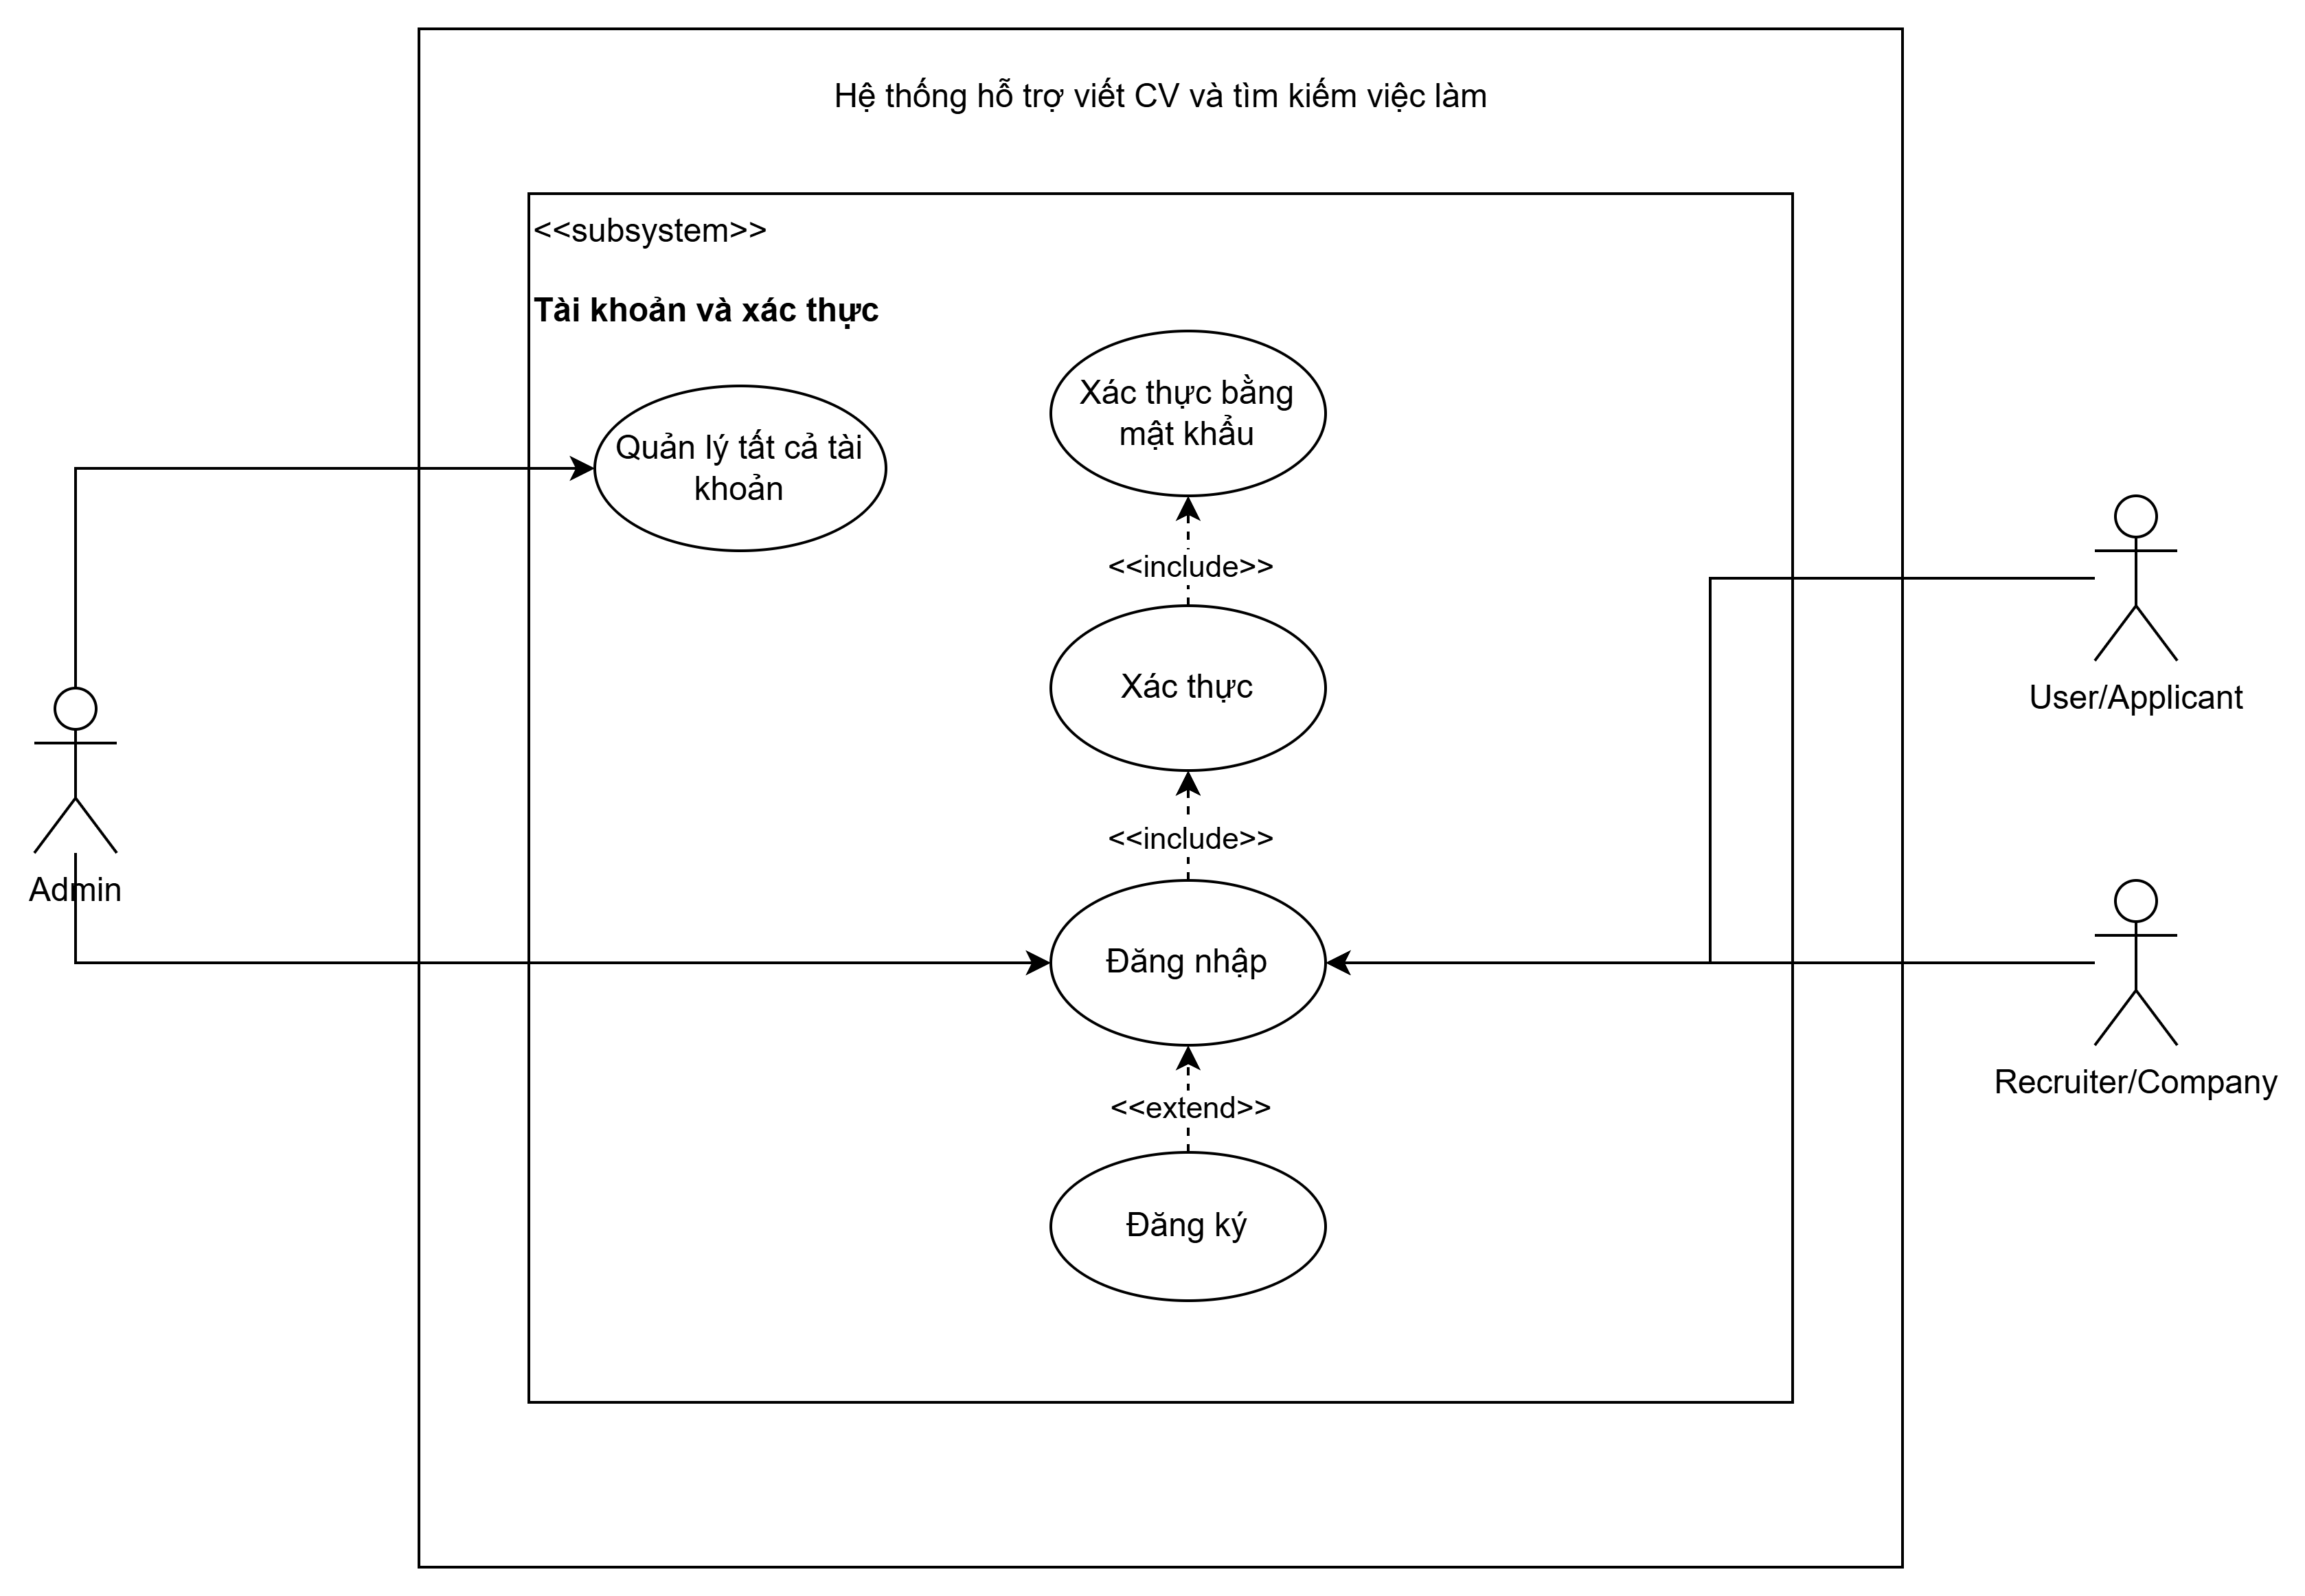
\includegraphics[scale=0.1]{img/AccountAuthenticationUsecase.png}
    \caption{Lược đồ usecase về Hệ thống tài khoản và xác thực}
\end{figure}

Hệ thống con này sẽ chịu trách nhiệm cho việc quản lý tài khoản, mật khẩu của người dùng và quản lý quá trình xác thực của tài khoản, bao gồm việc đăng ký và đăng nhập của tài khoản. Hệ thống sẽ xác thực tài khoản thông qua kiểm tra mật khẩu đã được lưu giữ trước đó ở trong dữ liệu khi lúc đăng ký tạo tài khoản.


\subsubsection{Hệ thống giao tiếp và quản lý thông tin}

\begin{figure}[H]
	\centering
    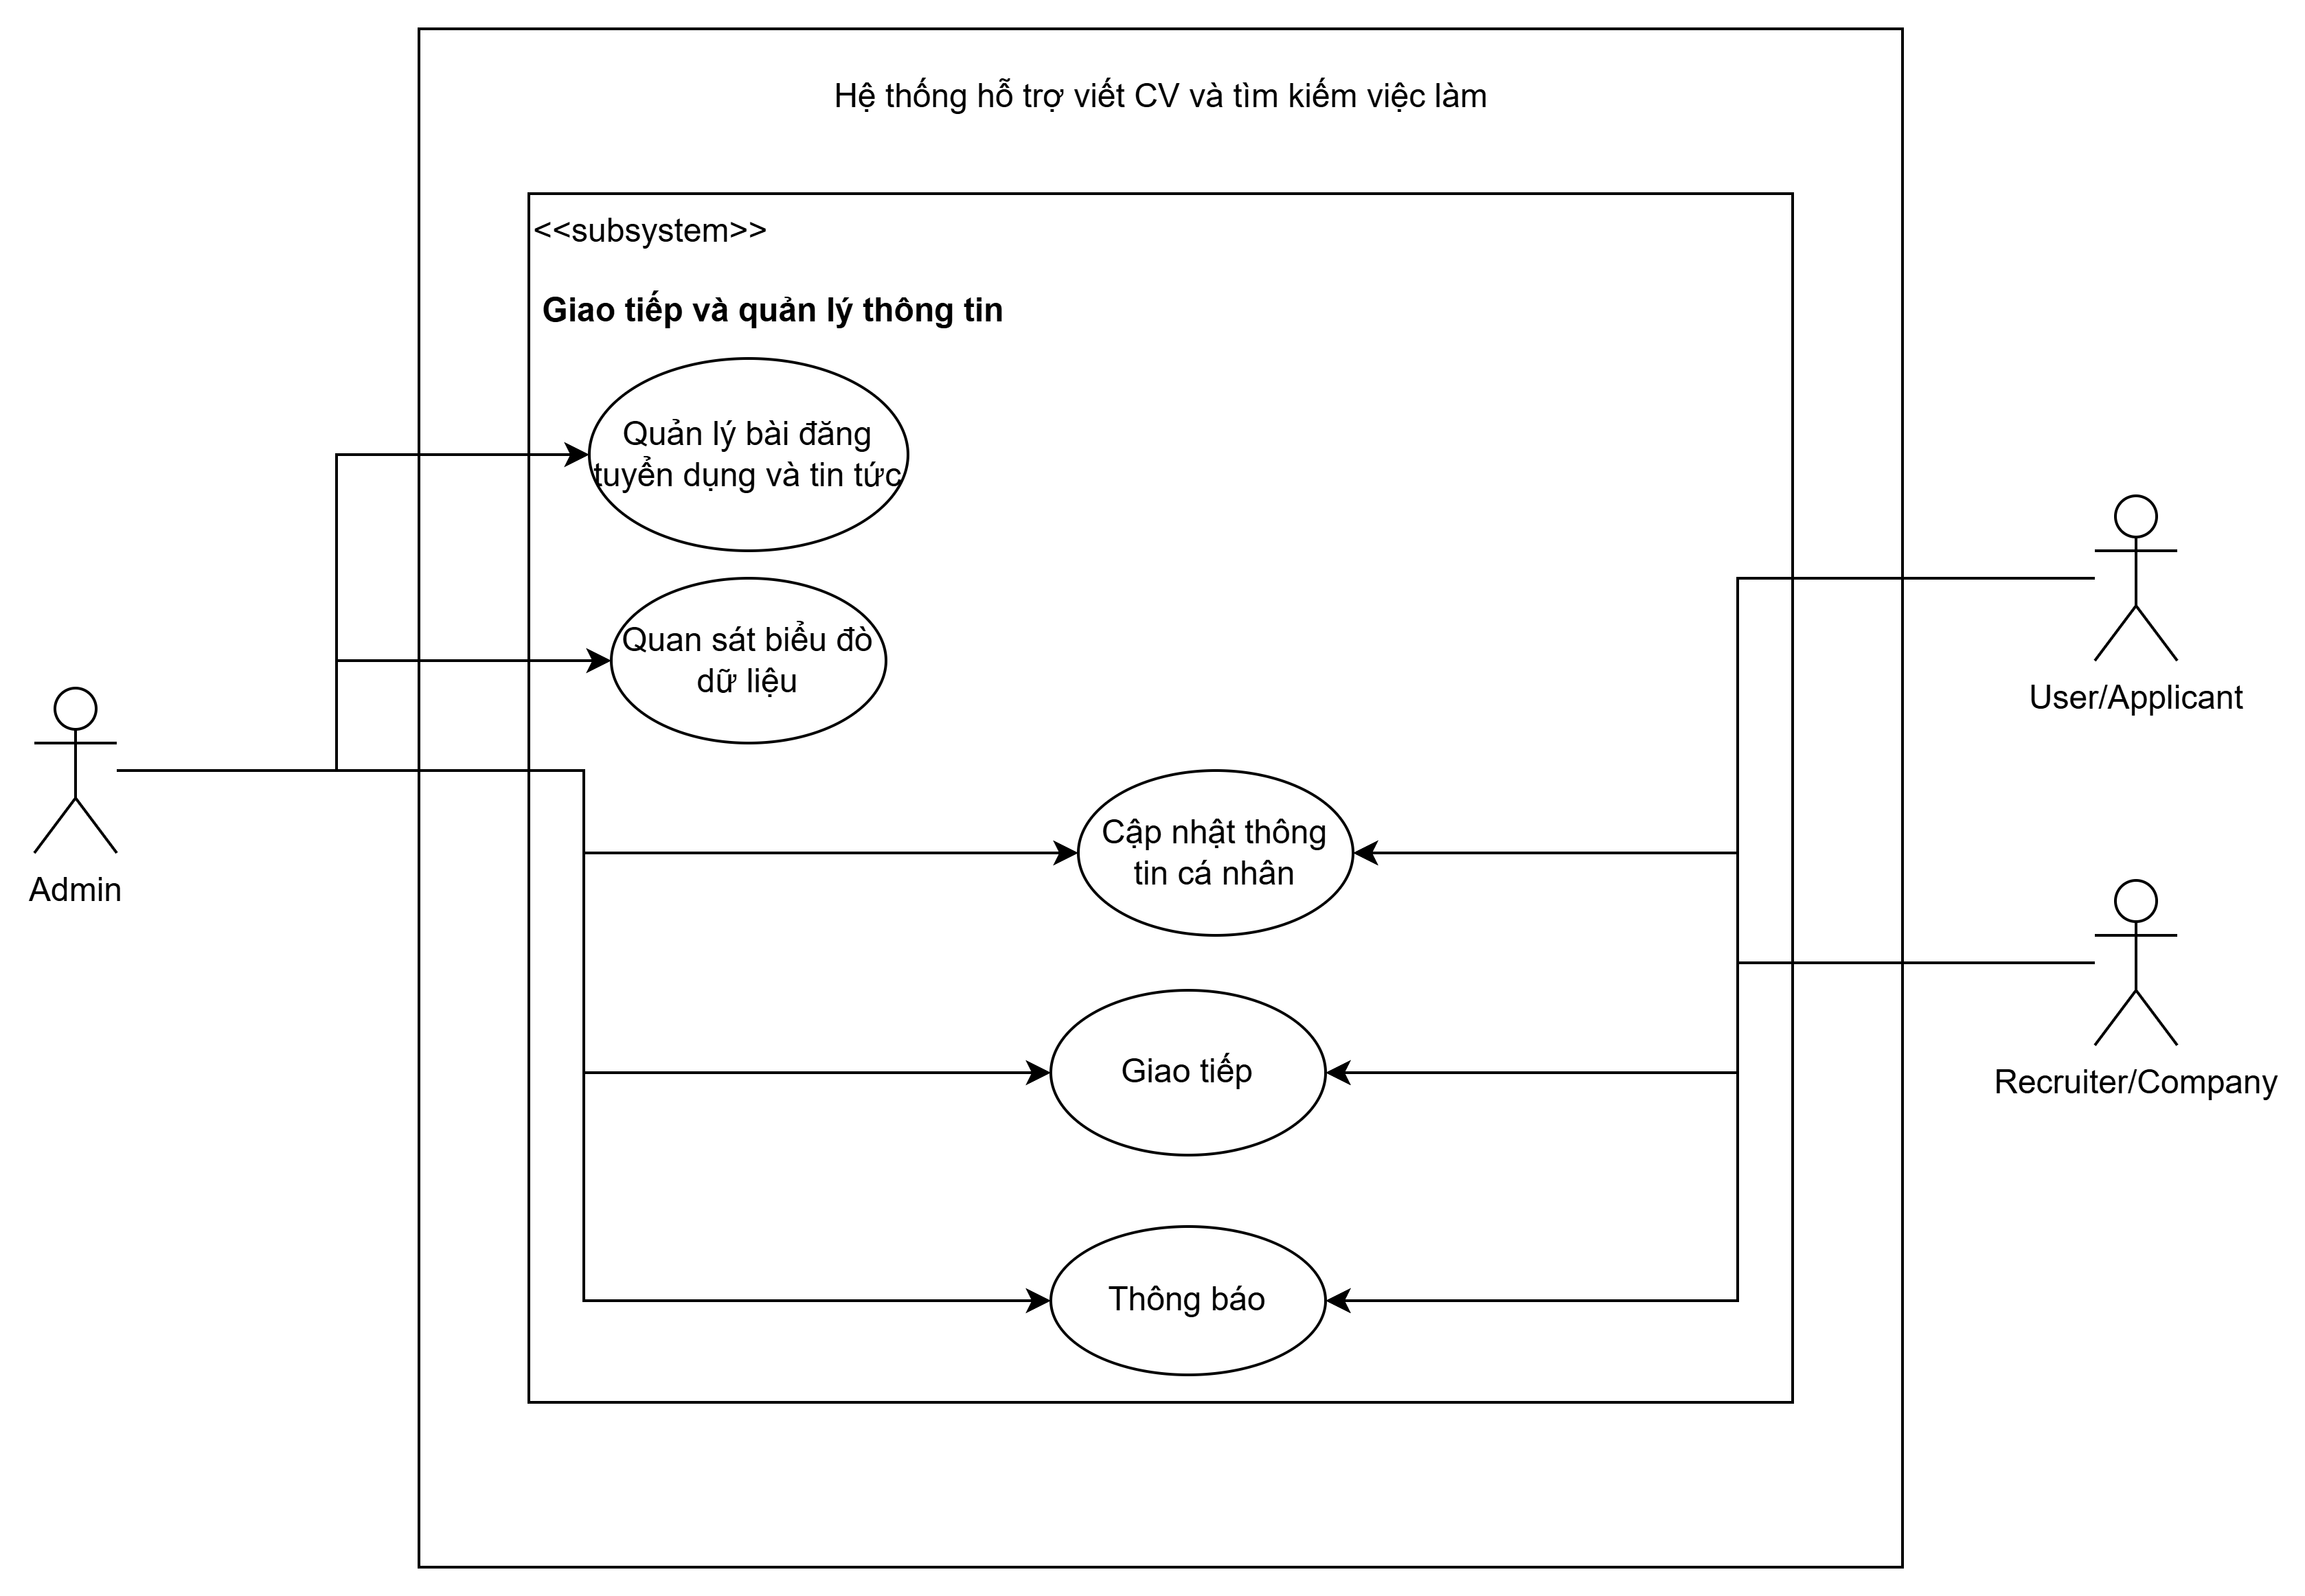
\includegraphics[scale=0.1]{img/communicateInfomationUsecase.png}
    \caption{Lược đồ usecase về Hệ thống giao tiếp và quản lý thông tin}
\end{figure}

Hệ thống sẽ đảm nhiệm vai trò trong việc lưu trữ và truyền tải tin nhắn giữa người với người. Đồng thời, hệ thống này cũng sẽ chịu trách nhiệm trong việc quản lý thông tin người dùng, trong việc chỉnh sửa và cập nhật thông tin cá nhân người dùng.

Đối với admin, hệ thống sẽ chuyển đổi toàn bộ dữ liệu thành bảng biểu, thông số giúp admin có thể dễ dàng tìm hiểu được tình trạng hiện tại của trang web. Admin cũng quản lý những bài đăng, tin tức sẽ xuất hiện trên trang web.


\subsubsection{Hệ thống truy xuất dữ liệu}

\begin{figure}[H]
	\centering
    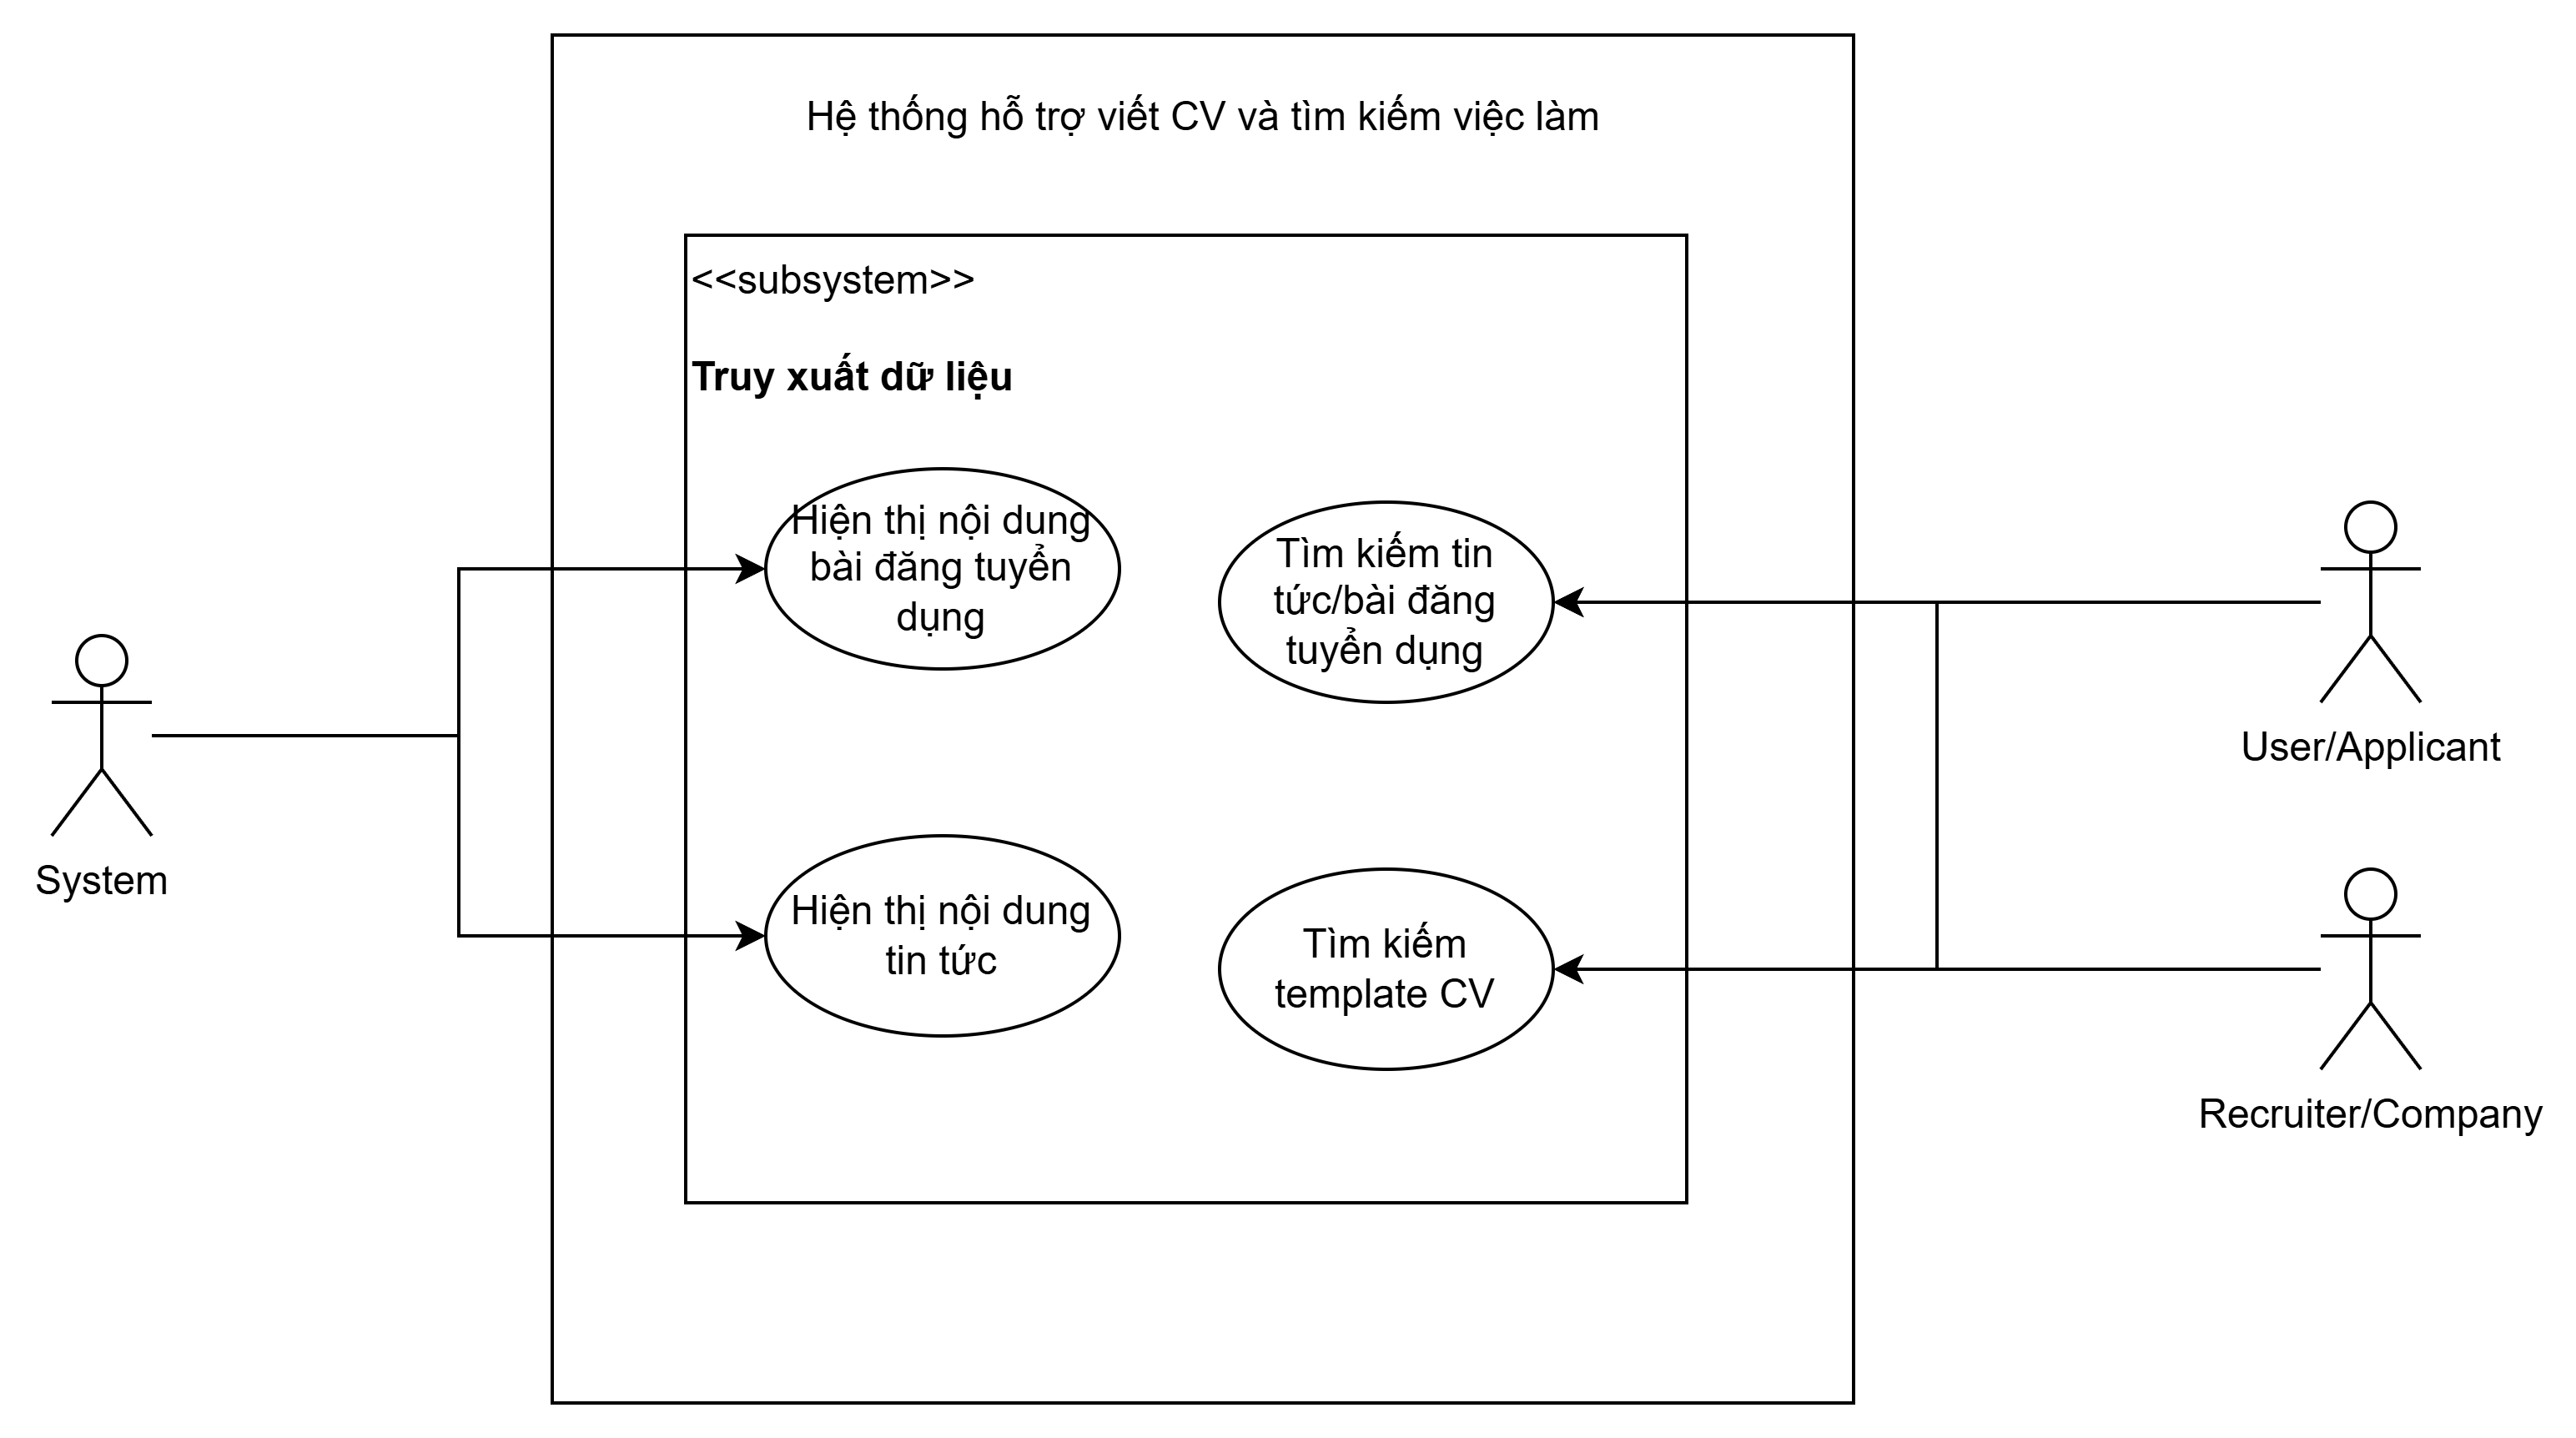
\includegraphics[scale=0.1]{img/TruyXuatDuLieu_Usecase.png}
    \caption{Lược đồ usecase về Hệ thống truy xuất dữ liệu}
\end{figure}

Đây là hệ thống truy xuất dữ liệu. Nơi mà sẽ chịu trách nhiệm cho hiển thị các nội dung có trong trang web như: các bài đăng tuyển dụng, tin tức, CV,.... Đối với người dùng, khi tìm kiếm tin tức hoặc bài đăng tuyển dụng nào hay bất kể template của CV nào, hệ thống sẽ cho hiển thị các nội dung tương ứng lên trang web.

\subsubsection{Lược đồ Usecase tổng quát }
\begin{figure}[H]

	\centering
     \includegraphics[scale = 0.05]{img/overview_usecase.png}
    \caption{Lược đồ usecase tổng quát}
\end{figure}

\url{https://drive.google.com/file/d/1gkpz6ht6IELJw3Rjp8x4X7RPldDnRzsi/view?usp=sharing}


Đây là lược đồ usecase tổng quát của hệ thống trang web hỗ trợ viết CV và tìm kiếm việc làm. Nó thể hiện các chức năng, tác vụ của người dùng, admin và nhà tuyển dụng. Hệ thống này sẽ bao gồm các hệ thống con kể trên nhưng sẽ không chi tiết như vậy. Lược đồ này sẽ mô tả sơ qua các chức năng chính của các bên liên quan chính (internal stakeholders). 

\subsection{Đặc tả lược đồ usecase}


\subsubsection{Đăng ký tài khoản (sử dụng mật khẩu)}


\begin{table}[H]
    \centering
    \begin{tabular}{|>{\centering\arraybackslash}p{0.3\linewidth}|>{\raggedright\arraybackslash}p{0.7\linewidth}|} \hline 
         ID& 1\\ \hline 
         Tên lược đồ usecase& Đăng ký tài khoản\\ \hline 
         Actors& User (Applicant)\\ \hline 
         Mô tả& Người dùng tạo một tài khoản mới ở đây\\ \hline 
         Tiền điều kiện (Pre-conditions)& Người dùng chưa có tài khoản.
Người dùng đang ở trang đăng ký tạo tài khoản mới.\\ \hline 
 Hậu điều kiện (Post-conditions)&Người tạo tài khoản mới thành công.\\\hline 
         Luồng thực thi chính (Normal flow)& 1. Người dùng vào trang tạo tài khoản mới.

2. Trang web sẽ hiện thị nội dung cần phải điền khi tạo tài khoản.

3. Người dùng điền thông tin vào.

4. Hệ thống kiểm tra liệu tài khoản đã có hay chưa.

5. Nếu tài khoản chưa có, thì thông báo tài khoản của người dùng được tạo thành công.\\ \hline 
         Luồng thực thi thay thế (Alternative flow)& \\ \hline 
         Luồng thực thi ngoại lệ (Exception flow)& 5.1.1. Ở bước thứ 5 nếu hệ thống kiểm tra tài khoản đã có rồi thì hệ thống sẽ hiển thị thông báo "Tài khoản đã có người dùng khác sử dụng".

5.1.2. Người dùng đổi lại tên tài khoản. Sau đó quay trở lại bước 4.\\ \hline
    \end{tabular}
    \caption{Bảng đặc tả usecase cho Đăng ký tài khoản}
    \label{tab:Register}
\end{table}



\subsubsection{Đăng nhập tài khoản}


\begin{table}[H]
    \centering
    \begin{tabular}{|>{\centering\arraybackslash}p{0.3\linewidth}|>{\raggedright\arraybackslash}p{0.7\linewidth}|} \hline 
         ID
& 2\\ \hline 
         Tên lược đồ usecase
& Đăng nhập tài khoản bằng mật khẩu\\ \hline 
         Actors
& Admin, user, company/recruiter\\ \hline 
         Mô tả
& Người dùng cố gắng đăng nhập vào hệ thống.\\ \hline 
         Tiền điều kiện (Pre-conditions)
& Người dùng đã có tài khoản hoặc đã tạo tài khoản trước đó.
Người dùng đang ở trang đăng nhập.\\ \hline 
         Hậu điều kiện (Post-conditions)
& Người dùng đăng nhập vô hệ thống thành công.\\ \hline 
         Luồng thực thi chính (Normal flow)
& 1. Người dùng vào trang đăng nhập.

2. Hệ thống hiển thị trang đăng nhập.

3. Người dùng điền tài khoản và mật khẩu vào trang web.

4. Hệ thống kiểm tra thông tin tài khoản và mật khẩu của người dùng liệu có khớp với dữ liệu được lưu trữ hay không.

5. Nếu khớp, hệ thống chuyển trang cho người dùng đến trang chủ của trang web và thông báo "Người dùng đã đăng nhập thành công.".\\ \hline 
         Luồng thực thi thay thế (Alternative flow)
& \\ \hline
 Luồng thực thi ngoại lệ (Exception flow)&5.1.1. Nếu hệ thống kiểm tra thông tin tài khoản và mật khẩu của người dùng không khớp thì người dùng sẽ được đưa về lại trang đăng nhập và được thông báo rằng "Tài khoản/Mật khẩu của người dùng không đúng."

5.1.2. Người dùng điền lại thông tin tài khoản và mật khẩu và quay lại bước 4.\\\hline
    \end{tabular}
    \caption{Bảng đặc tả usecase cho Đăng nhập tài khoản}
    \label{tab:Đăng nhập tài khoản}
\end{table}


\subsubsection{Tìm kiếm và chọn CV Template}

\begin{table}[H]
    \centering
    \begin{tabular}{|>{\centering\arraybackslash}p{0.3\linewidth}|>{\raggedright\arraybackslash}p{0.7\linewidth}|} \hline 
         ID
& 3\\ \hline 
         
Tên lược đồ usecase
& Tìm kiếm và chọn lựa template CV\\ \hline 
         Actors
& User\\ \hline 
         
Mô tả
& Người dùng tìm kiếm và chọn lựa các template của CV dựa trên CV có sẵn trên hệ thống.\\ \hline 
         Tiền điều kiện (Pre-conditions)
& Người đăng nhập vào tài khoản thành công\\ \hline 
         
Hậu điều kiện (Post-conditions)& Người dùng chọn lựa template CV thành công\\ \hline 
         Luồng thực thi chính (Normal flow)& 1. Người dùng vào trang CV của mình và chọn mục Template

2. Người dùng tìm kiếm và chọn cho mình template CV thích hợp với mình.

3. Sau đó người dùng đặt tên cho CV của mình và điền vào CV những thông tin mà CV yêu cầu theo từng ô được chỉ định.

4. Người dùng lưu lại CV. Nếu lưu lại CV thành công, hệ thống sẽ thông báo cho người dùng "Lưu CV thành công"\\ \hline 
         
Luồng thực thi thay thế (Alternative flow)
& Ở bước 2, nếu người dùng không tìm được CV ưng ý với mình. Người dùng có thể chọn mục Custom. Ở đây, người dùng có thể tự mình thiết kế CV phù hợp với mình nhất.\\ \hline
 Luồng thực thi ngoại lệ (Exception flow)&4.1 Nếu hệ thống lưu CV không thành công (do bởi kết nối mạng), hệ thống sẽ thông báo cho người dùng rằng: "Lưu CV thất bại do sự cố kết nối."\\\hline
    \end{tabular}
    \caption{Bảng đặc tả usecase cho Tìm kiếm và chọn lựa CV Template}
    \label{tab:Tìm kiếm và chọn CV templates}
\end{table}



\subsubsection{Quản lý CV}

\begin{table}[H]
    \centering
    \begin{tabular}{|>{\centering\arraybackslash}p{0.3\linewidth}|>{\raggedright\arraybackslash}p{0.7\linewidth}|} \hline 
         ID
& 4\\ \hline 
         
Tên lược đồ usecase
& Quản lý CV\\ \hline 
         Actors
& User\\ \hline 
         
Mô tả
& Người dùng quản lý (thêm, xoá, sửa) CV của mình.\\ \hline 
         Tiền điều kiện (Pre-conditions)
& Người dùng đã tạo tài khoản thành công.\\ \hline 
         
Hậu điều kiện (Post-conditions)& Người dùng có thể quản lý CV của mình.\\ \hline 
         Luồng thực thi chính (Normal flow)& 1. Người dùng vào trang "CV của mình".

2. Người dùng chọn 1 bản CV để chỉnh sửa hoặc xoá.

3. Nếu người dùng chọn sửa, hệ thống sẽ đưa người dùng đến trang chỉnh sửa CV và người dùng sẽ dựa vào những công cụ mà trang web có mà chỉnh sửa.

4. Hệ thống lưu lại những sự thay đổi đối với CV bạn đã chọn\\ \hline 
         
Luồng thực thi thay thế (Alternative flow)
& 3.1. Nếu người dùng chọn xoá CV thì hệ thống sẽ xoá dữ liệu của bản CV đó ra khỏi hệ thống dữ liệu. Và hệ thống sẽ reload lại trang với những dữ liệu mới được cập nhật.\\ \hline
 Luồng thực thi ngoại lệ (Exception flow)&4.1. Nếu không có kết nối mạng hoặc lỗi kết nối, dữ liệu sẽ không được lưu.\\\hline
    \end{tabular}
    \caption{Bảng đặc tả usecase cho Quản lý CV}
    \label{tab: Quản lý CV}
\end{table}



\subsubsection{Tìm kiếm bài đăng tuyển dụng}

\begin{table}[H]
    \centering
    \begin{tabular}{|>{\centering\arraybackslash}p{0.3\linewidth}|>{\raggedright\arraybackslash}p{0.7\linewidth}|} \hline 
         ID
& 5\\ \hline 
         
Tên lược đồ usecase
& Tìm kiếm bài đăng tuyển dụng\\ \hline 
         Actors
& Users, recuiter, external stakeholders\\ \hline 
         
Mô tả
& Người dùng tìm kiếm bài đăng tuyển dụng từ các công ty.\\ \hline 
         Tiền điều kiện (Pre-conditions)
& \\ \hline 
         
Hậu điều kiện (Post-conditions)& Người dùng có thể tìm kiếm công việc dễ dàng và hợp ý mình.\\ \hline 
         Luồng thực thi chính (Normal flow)& 1. Người dùng vào trang "Tìm việc làm".

2. Hệ thống hiển thị trang "Tìm việc làm" và liệt kê các bài đăng tuyển dụng công việc hiện có.

3. Chọn thanh tìm kiếm trên trang web.

4. Điền tên công việc mà bản thân muốn tìm kiếm.

5. Hệ thống tìm kiếm từ dữ liệu những bài đăng tuyển dụng trùng tên với tên công việc đang tìm kiếm.

6. Sau khi tìm kiếm, hệ thống sẽ liệt kê ra trang web những bài đăng tuyển dụng. Người dùng có thể chọn các loại filter, sort theo ngày, giờ, địa điểm.\\ \hline 
         
Luồng thực thi thay thế (Alternative flow)
& \\ \hline
 Luồng thực thi ngoại lệ (Exception flow)&6.1. Nếu hệ thống không tìm thấy dữ liệu trùng với tên công việc mà mình đang tìm kiếm, hệ thống sẽ thông báo "Không tìm thấy thông tin trùng với tên bạn tìm kiếm".\\\hline
    \end{tabular}
    \caption{Bảng đặc tả usecase cho Tìm kiếm bài đăng tuyển dụng}
    \label{tab:Tìm kiếm bài đăng tuyển dụng}
\end{table}

\subsubsection{Ứng tuyển công việc}

\begin{table}[H]
    \centering
    \begin{tabular}{|>{\centering\arraybackslash}p{0.3\linewidth}|>{\raggedright\arraybackslash}p{0.7\linewidth}|} \hline 
         ID
& 6\\ \hline 
         
Tên lược đồ usecase
& Ứng tuyển công việc\\ \hline 
         Actors
& User\\ \hline 
         
Mô tả
& Người dùng ứng tuyển vào vị trí của bài đăng tuyển dụng.\\ \hline 
         Tiền điều kiện (Pre-conditions)
& Người đã tạo tài khoản thành công.

Người dùng đã có CV đầy đủ cho chính mình trên web hoặc upload CV có sẵn của bản thân mình.\\ \hline 
         
Hậu điều kiện (Post-conditions)& \\ \hline 
         Luồng thực thi chính (Normal flow)& 1. Người dùng chọn 1 bài đăng tuyển dụng phù hợp với mình.

2. Hệ thống sẽ hiển thị những thông tin chi tiết liên quan đến bài đăng tuyển dụng.

3. Người dùng chọn "Ứng tuyền" ở bên trong bài viết.

4. Nếu người đã có CV đầy đủ, hệ thống sẽ thông báo cho người dùng "Ứng tuyển thành công".\\ \hline 
         
Luồng thực thi thay thế (Alternative flow)
& \\ \hline
 Luồng thực thi ngoại lệ (Exception flow)&4.1. Nếu người dùng chưa có CV đầy đủ hoặc chưa upload CV của riêng mình thì hệ thống sẽ thông báo cho người dùng "Ứng tuyển thất bại" và di chuyển người dùng đến trang "Quản lý CV" của mình.\\\hline
    \end{tabular}
    \caption{Bảng đặc tả usecase cho Ứng tuyển công việc}
    \label{tab:Ứng tuyển công việc}
\end{table}

\subsubsection{Chia sẻ CV}

\begin{table}[H]
    \centering
    \begin{tabular}{|>{\centering\arraybackslash}p{0.3\linewidth}|>{\raggedright\arraybackslash}p{0.7\linewidth}|} \hline 
         ID
& 7\\ \hline 
         
Tên lược đồ usecase
& Chia sẻ CV\\ \hline 
         Actors
& User\\ \hline 
         
Mô tả
& Người dùng chia sẻ CV của mình đến những người dùng khác hoặc chia sẻ CV của mình đến các nhà tuyển dụng để họ tìm đến mình.\\ \hline 
         Tiền điều kiện (Pre-conditions)
& Người dùng tạo tài khoản thành công.

Người dùng đã có CV hoàn chỉnh hoặc upload CV của riêng mình.\\ \hline 
         
Hậu điều kiện (Post-conditions)& Người dùng chia sẻ CV đến mọi người thành công.\\ \hline 
         Luồng thực thi chính (Normal flow)& 1. Người dùng vào trang "Quản lý CV" của mình.

2. Người dùng chọn một CV mà mình ưng ý và muốn chia sẻ chúng.

3. Người dùng vào trang CV đó và ở góc phải, người chọn "Chia sẻ".

4. Hệ thống hiển thị ra 2 option cho người dùng chọn: "Chia sẻ đến người dùng khác" và "Chia sẻ tìm kiếm công việc".

5. Người dùng chọn 1 trong 2 option hoặc cả 2.

6. Nếu thành công, hệ thống thông báo đến người dùng "Chia sẻ thành công".\\ \hline 
         
Luồng thực thi thay thế (Alternative flow)
& 6.1. Nếu người dùng chọn option "Chia sẻ đến người dùng khác", sau khi chia sẻ thành công, người dùng có thể copy link CV của mình và gửi đến những người dùng khác.\\ \hline
 Luồng thực thi ngoại lệ (Exception flow)&\\\hline
    \end{tabular}
    \caption{Bảng đặc tả usecase cho Chia sẻ CV}
    \label{tab:Chia sẻ CV}
\end{table}





\section{Thiết kế quy trình làm việc (Workflow design)}


\subsection{Đăng ký tài khoản (Register)}

\begin{figure}[H]

	\centering
    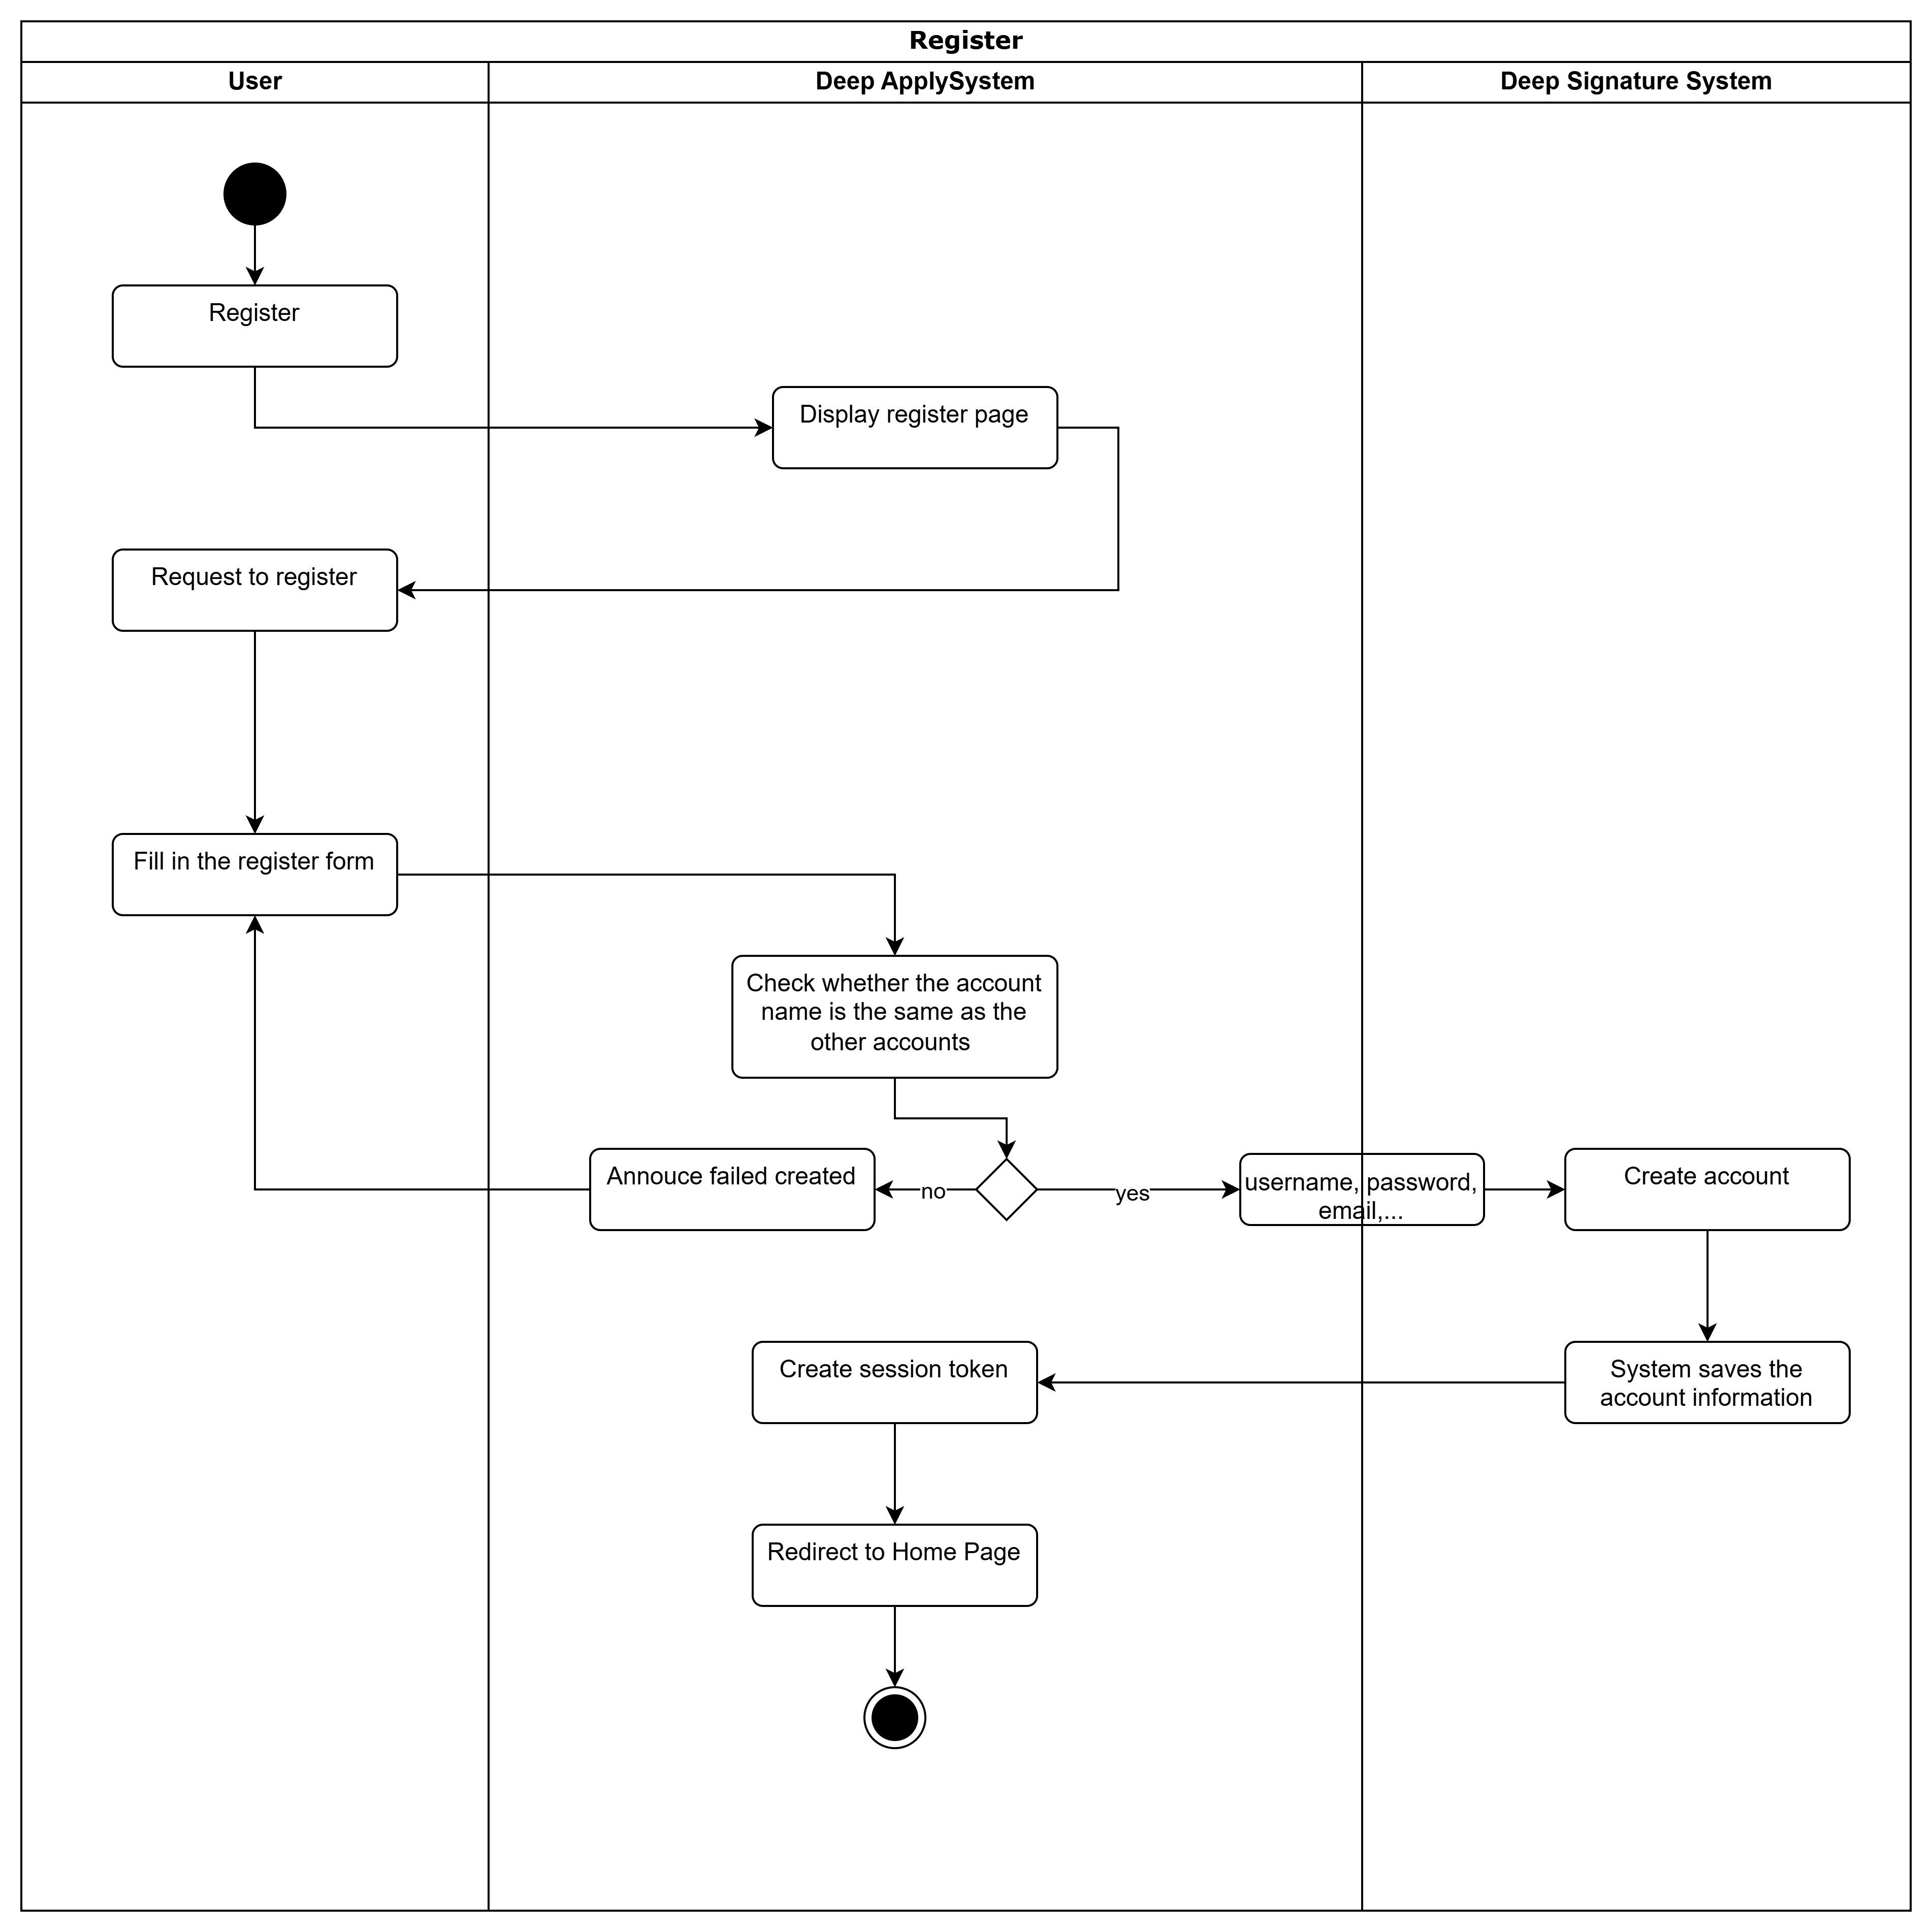
\includegraphics[scale=0.08]{img/Register_workflow.png}
    \caption{Lược đồ hoạt động về Đăng ký tài khoản}

\end{figure}

Biểu đồ trên mô tả quy trình làm việc của quá trình đăng ký tài khoản. Sau khi người dùng bấm vào nút Đăng ký, hệ thống sẽ đưa người dùng đến trang đăng ký tài khoản. Ở đây sẽ có 1 form yêu cầu những thông tin cần thiết của người dùng để có thể tạo tài khoản thành công. Sau khi điền thông tin xong, người dùng bấm vào nút "Đăng ký" bên dưới form. Sau đó hệ thống sẽ bắt đầu kiểm tra thông tin người dùng hợp lệ hay không. Sau khi hệ thống kiểm tra tài khoản của người dùng không bị trùng lặp với những tài khoản khác, người dùng sẽ được hệ thống thông báo tạo tài khoản thành công và chuyển hướng trang đến trang chủ. Còn nếu tài khoản bị trùng lặp, người dùng sẽ bị quay lại ở trang Đăng ký tài khoản và chỉnh sửa lại tên tài khoản sao cho không bị trùng lặp với những người dùng khác. Trong trường hợp người dùng chưa điền hết thông tin cần thiết, hệ thống sẽ hiển thị thông báo cho người dùng "Bạn chưa hoàn thành form thông tin đăng ký tài khoản". Sau khi tạo tài khoản thành công, toàn bộ thông tin người dùng sẽ được lưu trữ vào cơ sở dữ liệu của hệ thống.

\subsection{Đăng nhập tài khoản (Login)}

\begin{figure}[H]

	\centering
    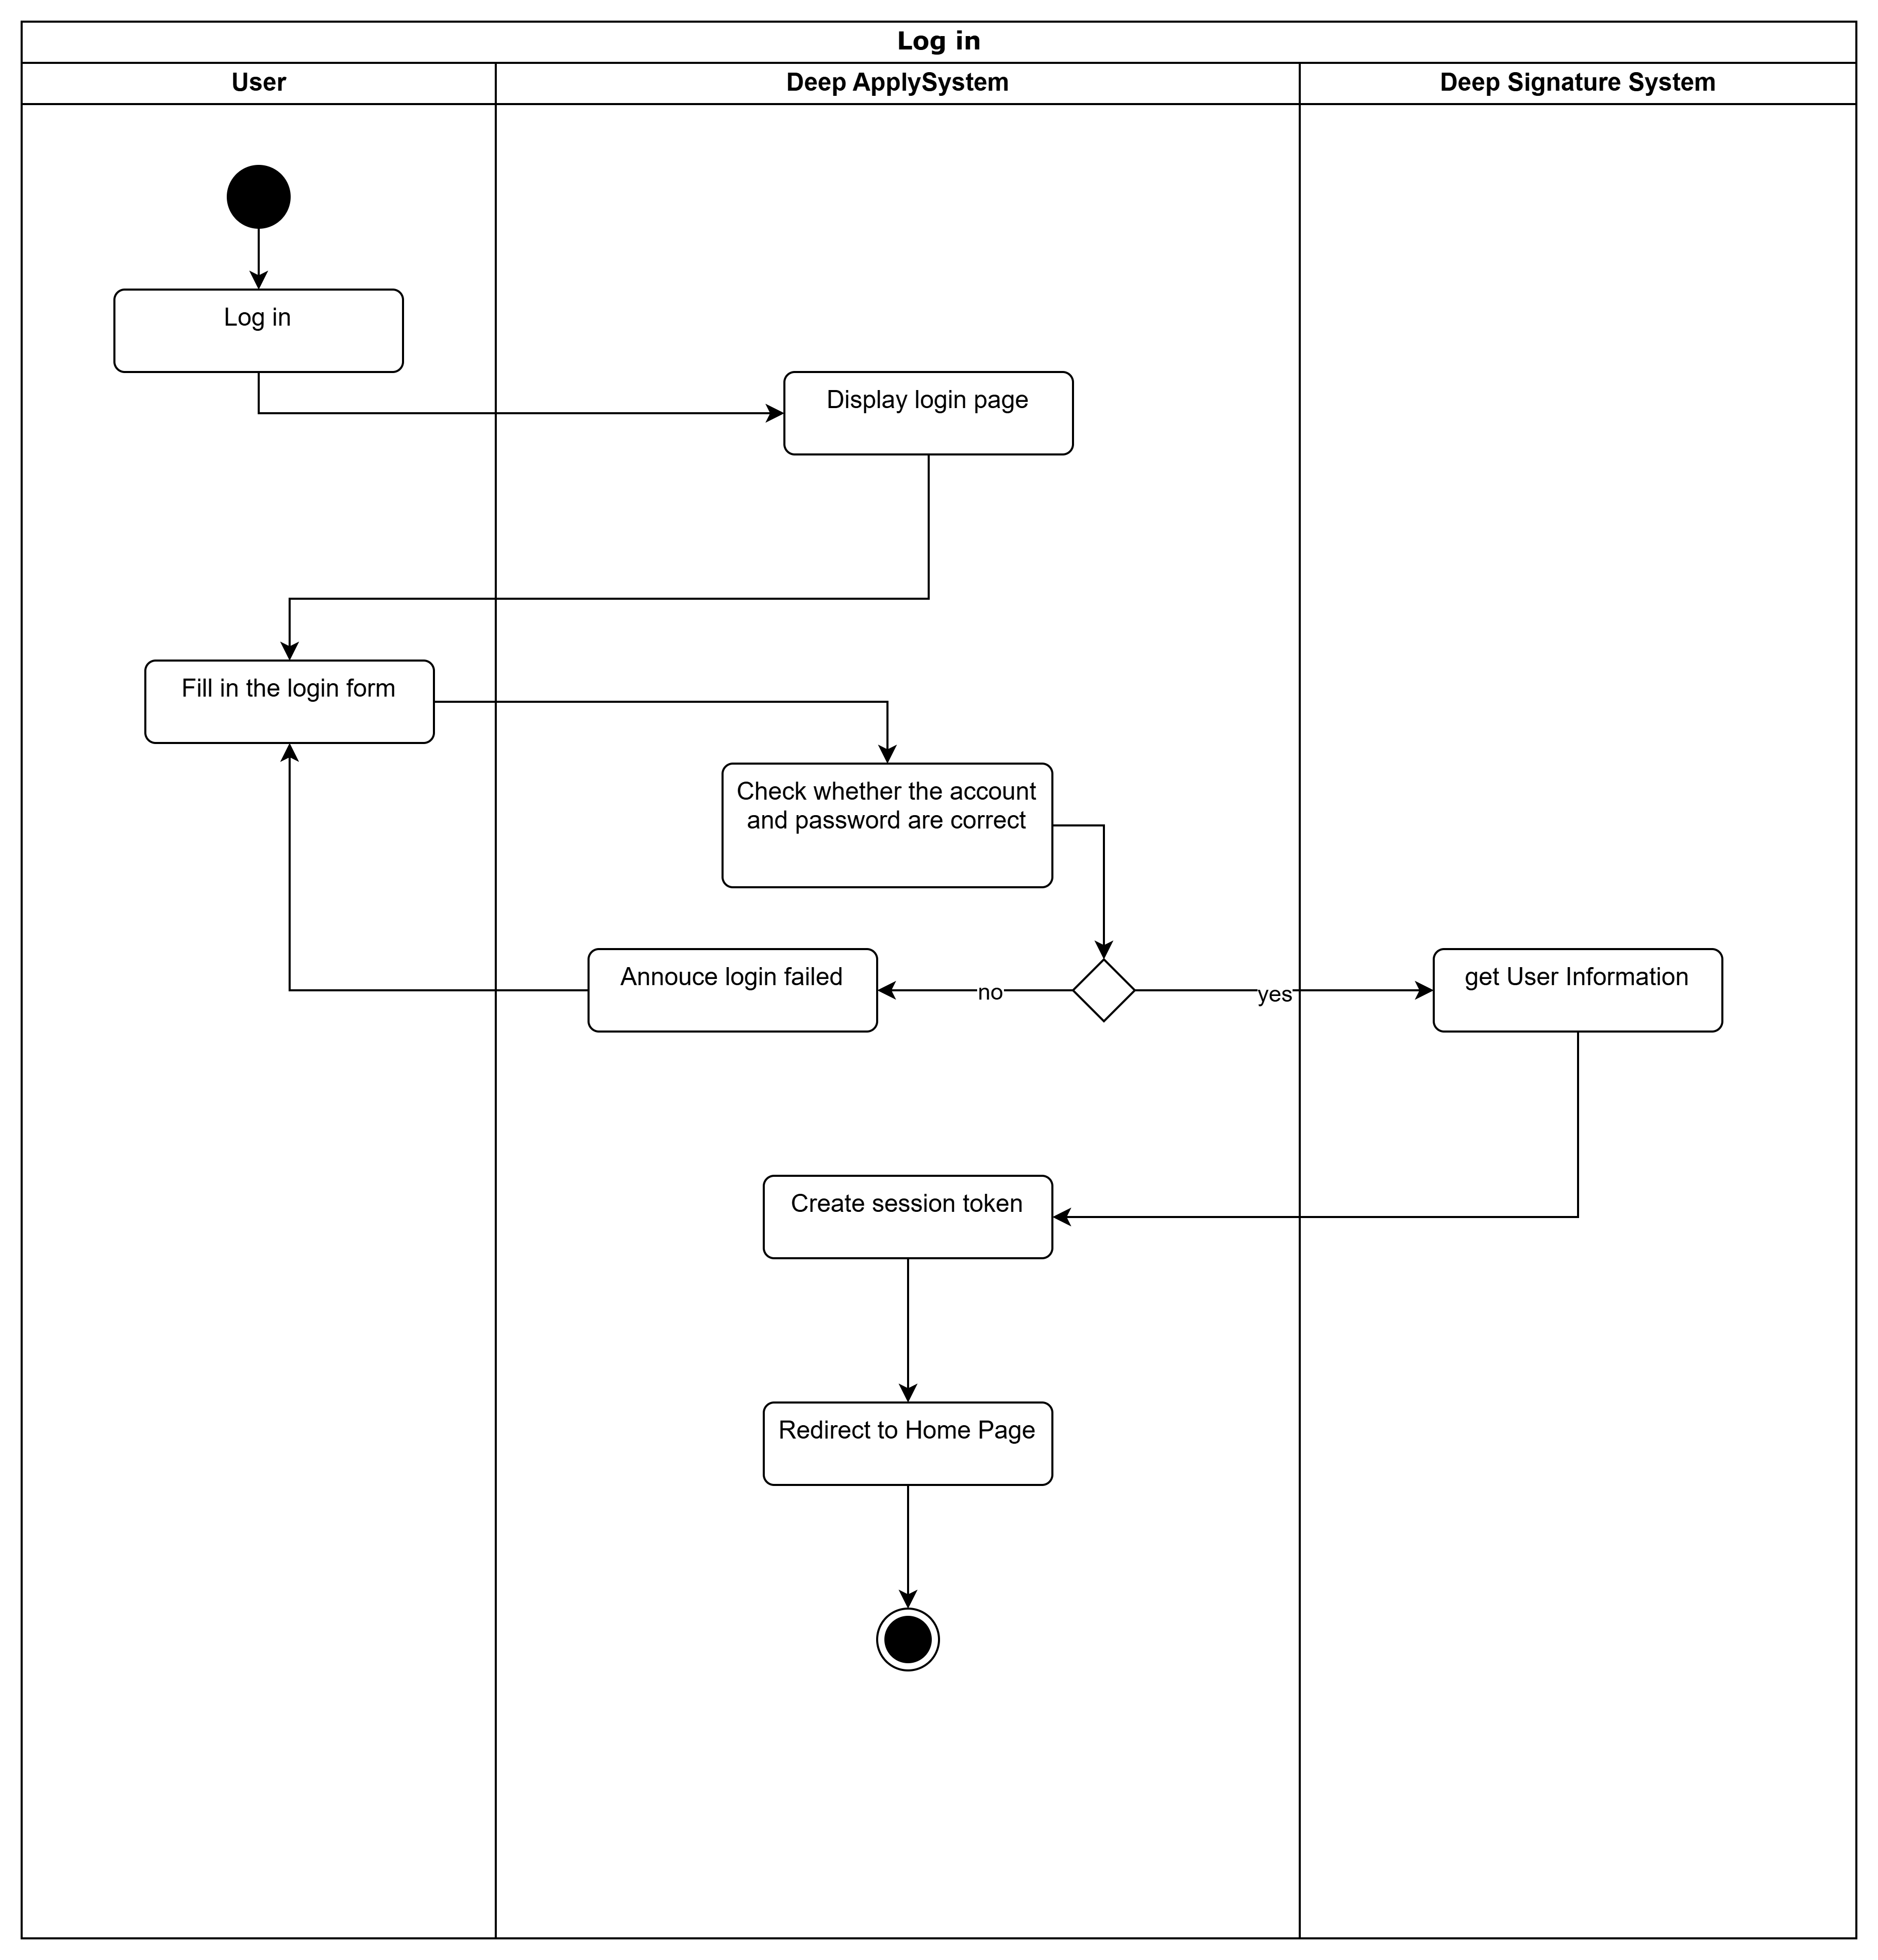
\includegraphics[scale=0.08]{img/Login_workflow.png}
    \caption{Lược đồ hoạt động về Đăng nhập tài khoản}
\end{figure}

Quy trình làm việc cho biểu đồ hoạt động của "Đăng nhập tài khoản": sẽ chia làm 2 đối tượng, một là những người sử dụng bình thường và còn lại là những tài khoản công ty được admin cung cấp để sử dụng. Người dùng lựa chọn 1 trong 2 option là "Người dùng" và "Doanh nghiệp". Sau đó sẽ được hệ thống đưa đến và hiển thị trang "Login page". Sau khi người dùng điền tài khoản và mật khẩu, hệ thống sẽ thực hiện chức năng xác thực, kiểm tra xem liệu người dùng điền thông tin tài khoản và mật khẩu trùng với dữ liệu hệ thống không? Nếu tài khoản và mật khẩu của người dùng trùng với dữ liệu của hệ thống, người dùng sẽ được hệ thống chuyển hướng tới trang "Trang chủ" của trang web.

Nếu tài khoản và mật khẩu của người dùng không khớp với bất kỳ dữ liệu của hệ thống, người dùng sẽ được hiển thị thông báo "Tài khoản hoặc mật khẩu của bạn không chính xác. Vui lòng kiểm tra lại." và bị giữ lại ở trang Đăng nhập. Người cũng có một lựa chọn khác là tạo một tài khoản mới với chức năng "Đăng ký tài khoản.". Quy trình làm việc của chức năng "Đăng ký tài khoản" đã được trình bày ở trên. Sau khi đăng nhập thành công, hệ thống sẽ tạo 1 session token và lưu giữ trên máy tính của người dùng nhằm duy trì trạng thái đăng nhập của người dùng.

\subsection{Ứng tuyển công việc (Apply jobs)}

\begin{figure}[H]

	\centering
    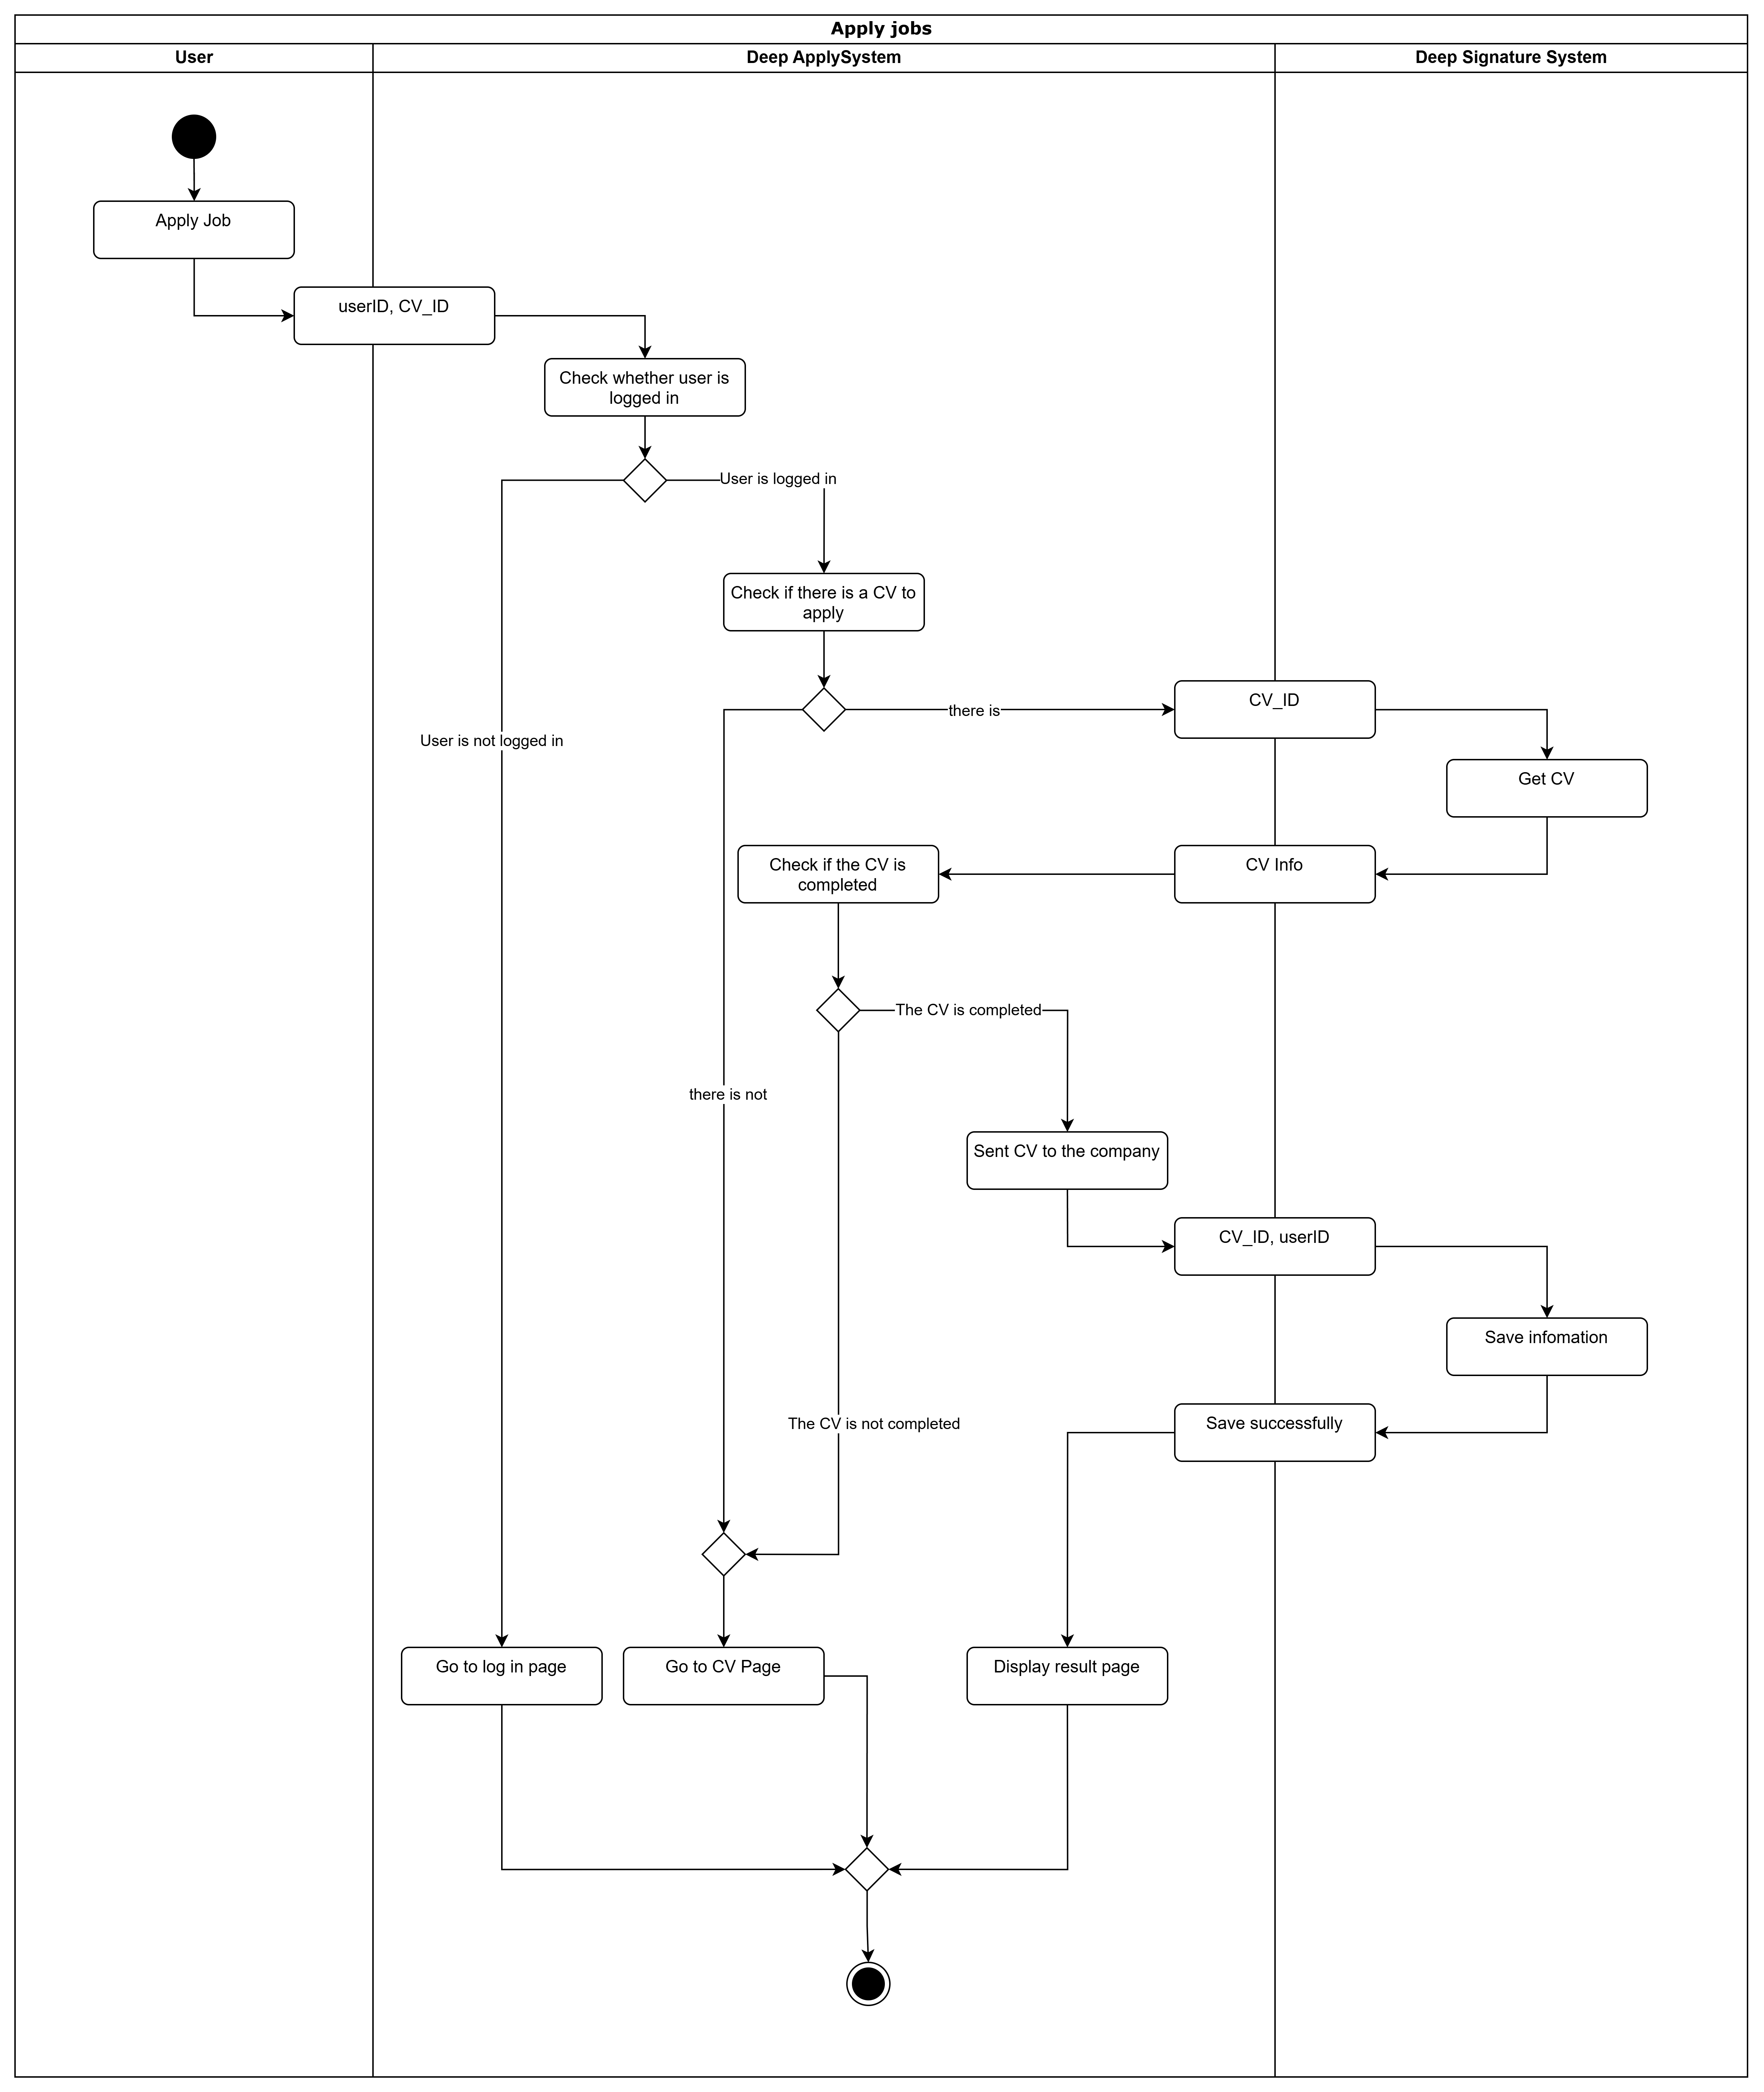
\includegraphics[scale=0.08]{img/Apply_jobs_Activity.png}
    \caption{Lược đồ hoạt động về Ứng tuyển công việc}
\end{figure}

Sau khi ứng tuyển cho một bài đăng tuyển dụng trên trang web, hệ thống sẽ kiểm tra người đã đăng nhập hay chưa. Nếu chưa người dùng được đến trang đăng nhập của trang web để thực hiện đăng nhập tài khoản. Thậm chí, nếu người dùng vẫn chưa có tài khoản trên trang web, người dùng có thể chọn phần "Đăng ký tài khoản" có trên trang Đăng nhập để thực hiện "Đăng ký tài khoản". 

Khi người dùng đăng nhập tài khoản thành công, hệ thống sẽ kiểm tra người dùng đã có CV đang trong tình trạng "Ứng tuyển" hay chưa? Trong trường hợp không có, người dùng được đưa đến trang "Quản lý CV" và cần phải tạo và hoàn thiện 1 CV mới và cho CV sang tình trạng "Ứng tuyển". Hoặc người dùng cũng có thể upload một bản CV sẵn có của bản thân lên trang web và cho nó vô tình trạng "Ứng tuyển". Sau khi tạo CV mới hay upload một CV mới lên trang web thành công, hệ thống sẽ lưu thông tin của CV vào cơ sở dữ liệu của hệ thống. 

Sau khi bấm vào nút "Ứng tuyển" trên bài đăng tuyển dụng và đã có bản CV đang trong tình trạng "Ứng tuyển", hệ thống sẽ tự động gửi thông tin và CV ứng tuyển của người dùng cho doanh nghiệp và lưu chúng vào một danh sách ứng tuyển của doanh nghiệp. Sau đó, hệ thống sẽ thông báo cho người dùng "Ứng tuyển thành công" và chuyển hướng đến trang chủ của trang web.

\subsection{Đăng bài tuyển dụng/tin tức}


\begin{figure}[H]

	\centering
    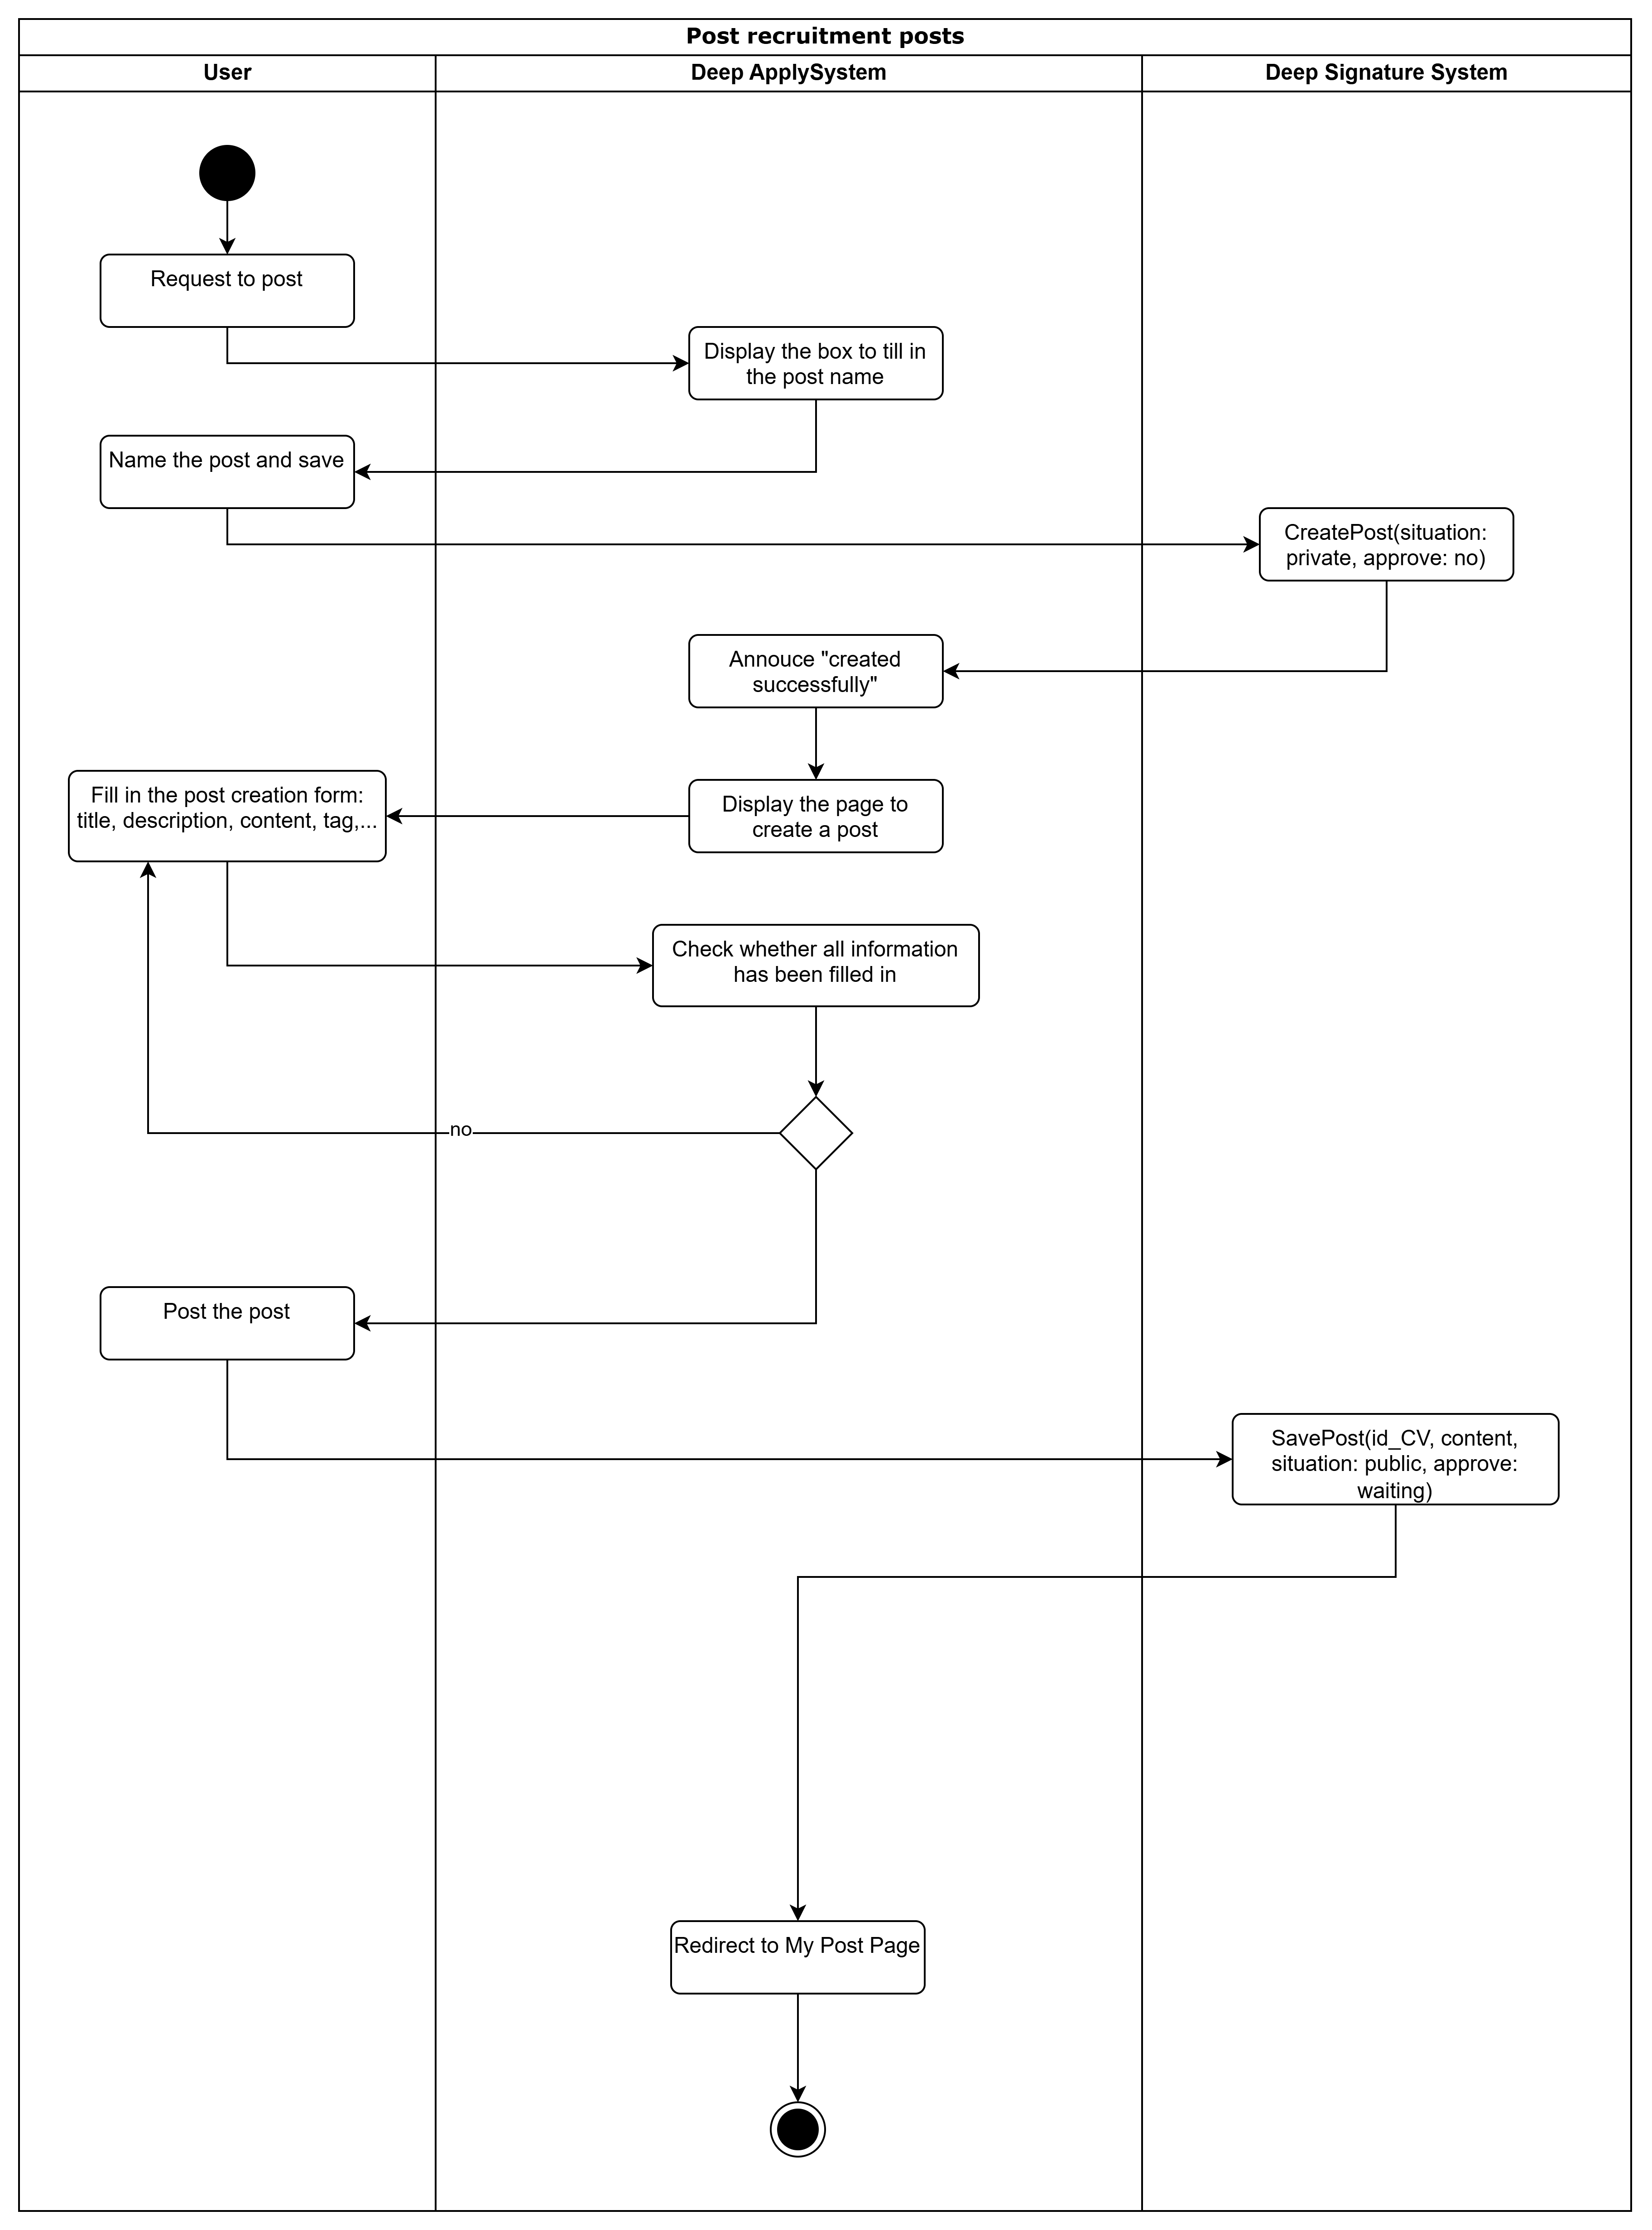
\includegraphics[scale=0.07]{img/Post_workflow.png}
    \caption{Lược đồ hoạt động về Đăng bài tuyển dụng/tin tức}
\end{figure}

Quy trình làm việc cho biểu đồ hoạt động của đăng bài tuyển dụng: Khi được yêu cầu đăng bài tuyển dụng, hệ thống sẽ hiển thị cho người dùng một trang web để đăng các bài tuyển dụng. Khi này, hệ thống sẽ cho rằng bản đang hiển thị trên trang web là bản nháp và không lưu lại vào cơ sở dữ liệu của hệ thống. Khi người dùng đặt tên cho bài đăng, hệ thống sẽ tạo và lưu dữ liệu của bài đăng vào cơ sở dữ liệu của người dùng.Ở đây, người dùng cần điền những thông tin cho bài đăng bao gồm: tiêu đề, mô tả, nội dung, yêu cầu, hình ảnh,.... 

Khi người dùng bấm vào nút đăng ở phía trên của form, hệ thống sẽ kiểm tra liệu người dùng đã điền hoàn tất chưa. Nếu người dùng chưa hoàn tất thông tin cần có, hệ thống sẽ thông báo cho người dùng "Đăng bài thất bại. Xin hãy hoàn thiện nội dung của bài đăng tuyển dụng". Nếu đã hoàn thiện nội dung của bài đăng, hệ thống sẽ thông báo cho người dùng "Đăng bài thành công. Xin vui lòng chờ admin duyệt”. Bài đăng sẽ được chuyển đến admin và chờ admin duyệt để có thể bài đăng tuyển dụng có thể thật sự xuất hiện trên trang web.



\subsection{Gửi tin nhắn}

\begin{figure}[H]

	\centering
    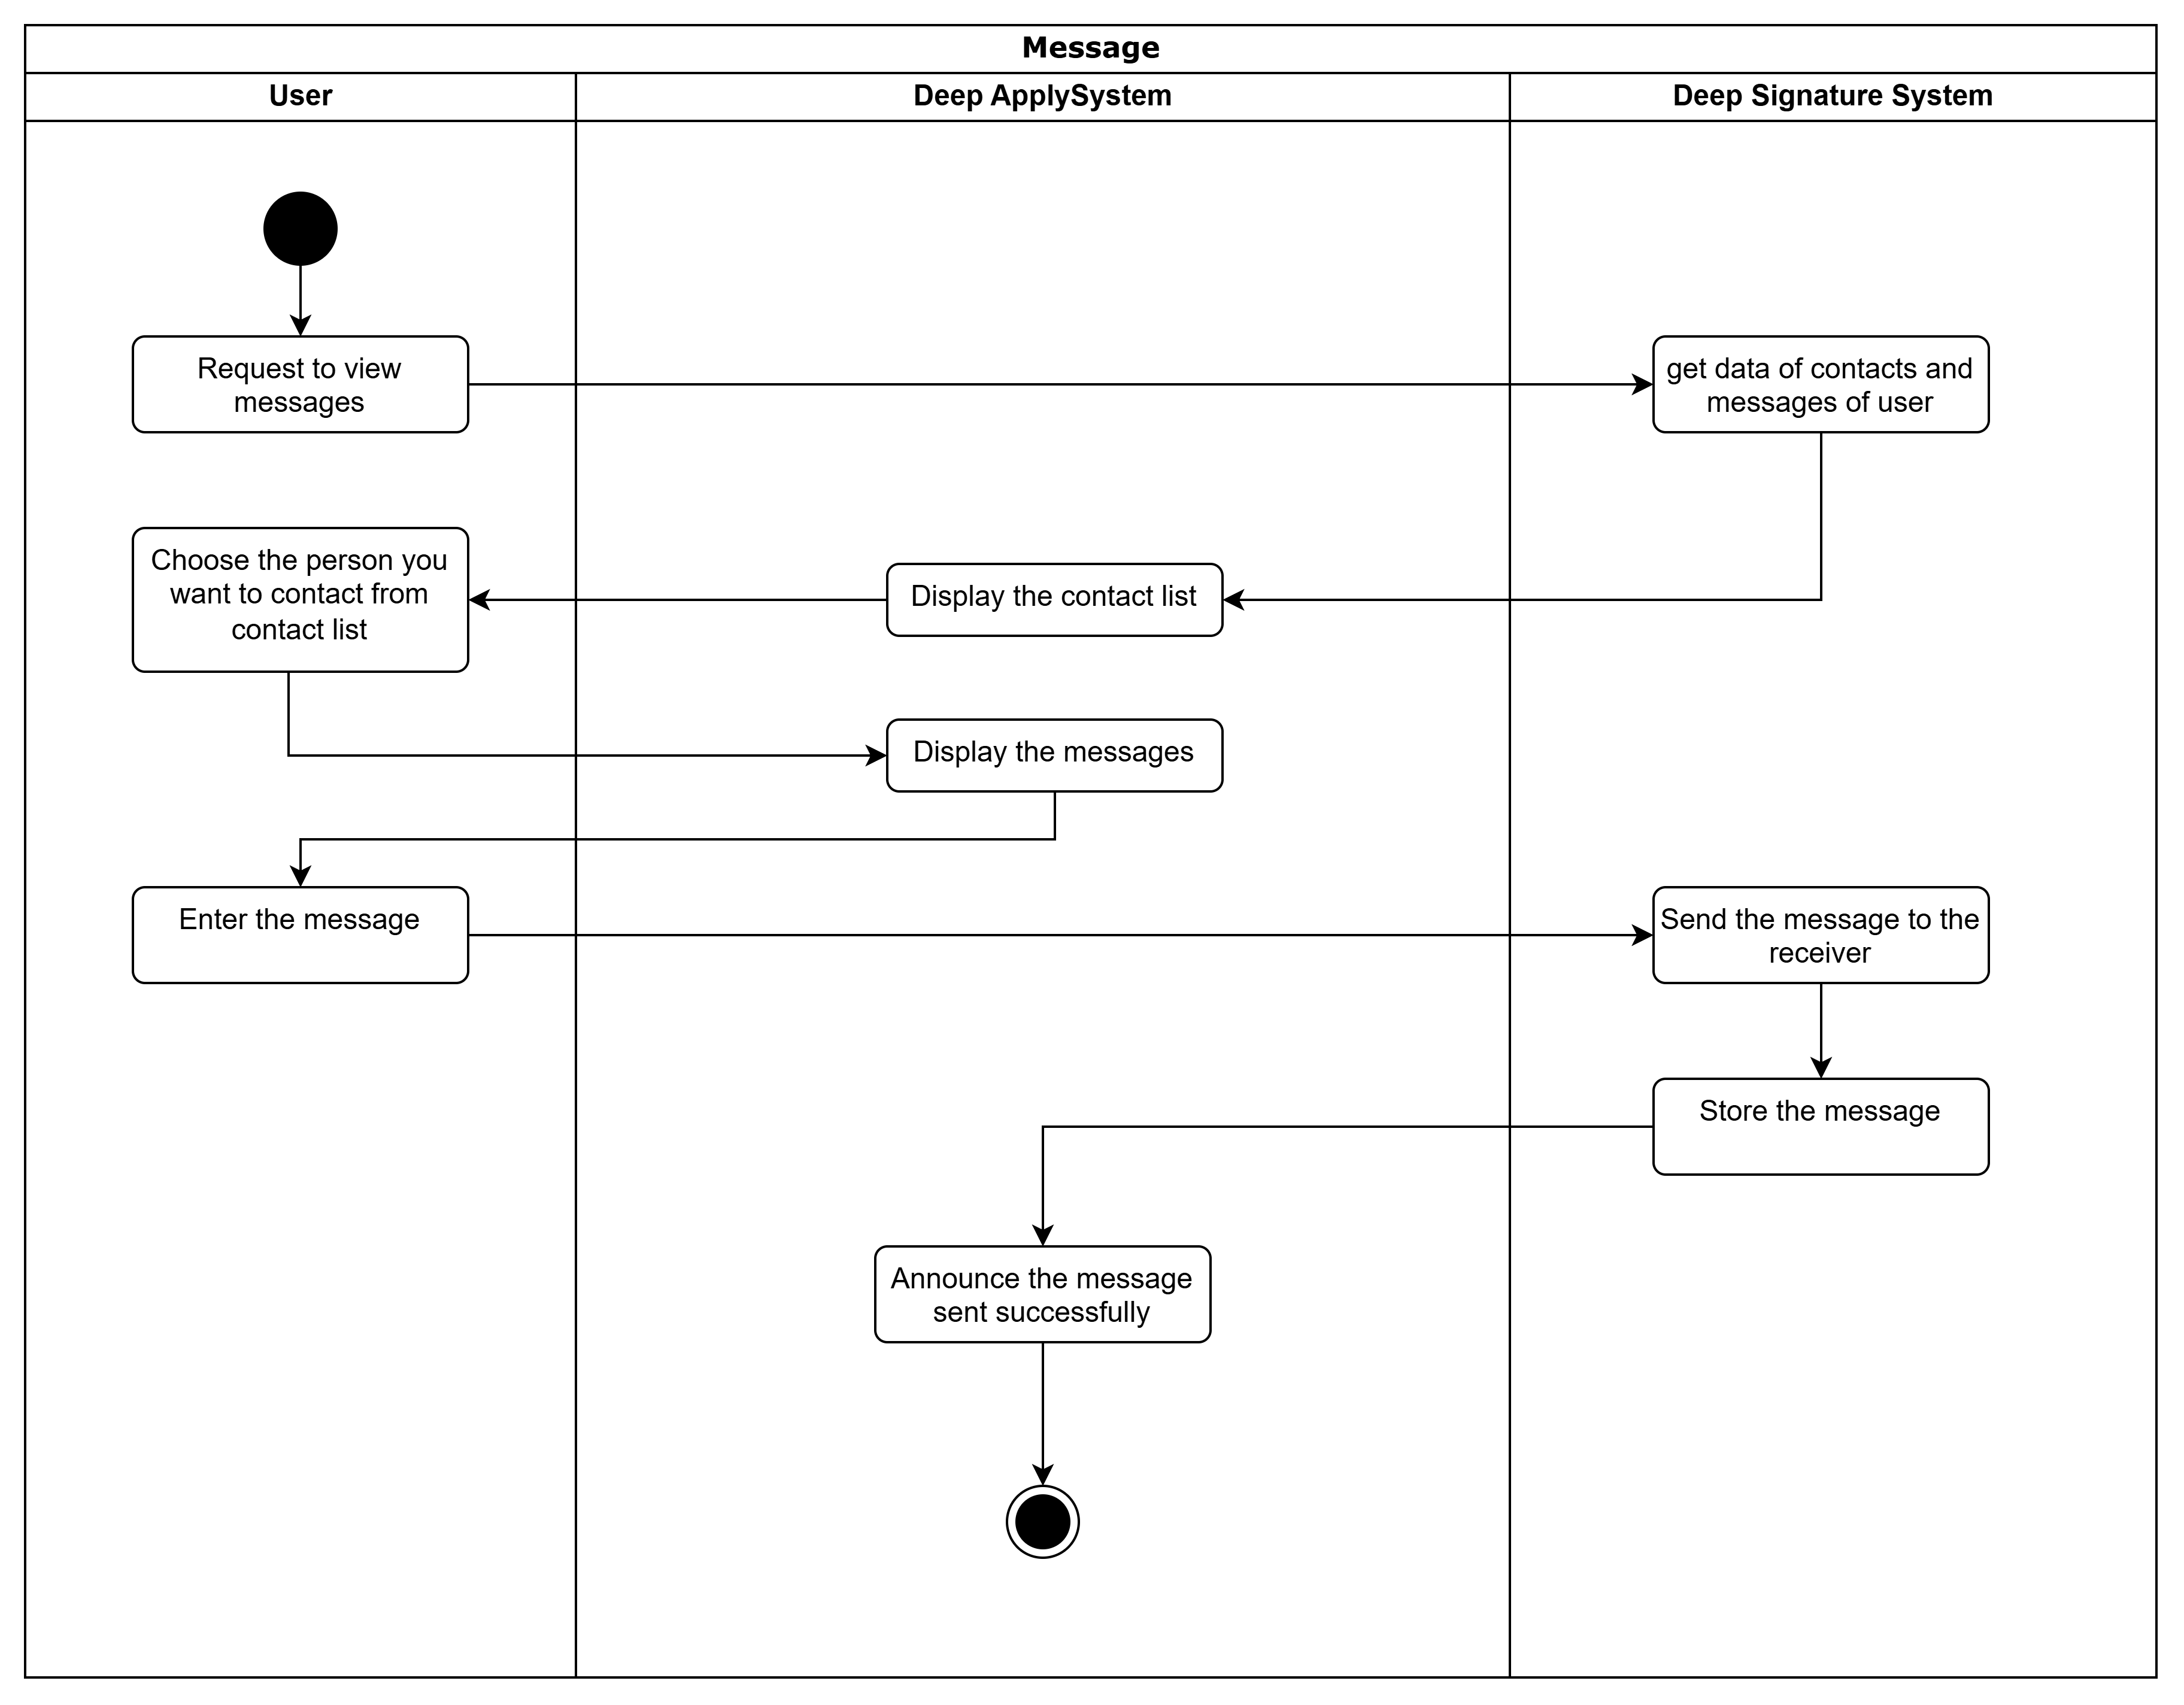
\includegraphics[scale=0.1]{img/Message_workflow.png}
    \caption{Lược đồ hoạt động về Gửi tin nhắn}
\end{figure}

Khi người dùng vào mục nhắn tin, hệ thống sẽ lấy toàn bộ tin nhắn của người dùng với những người khác và hiển thị cho người dùng danh sách những người mà họ đã giao tiếp. Người dùng sẽ chọn một người trong danh sách liên lạc. Hệ thống sẽ hiển thị cho người dùng toàn bộ tin nhắn giữa hai người. Khi người dùng gửi tin nhắn, hệ thống sẽ gửi tin nhắn đến người nhận và lưu giữ tin nhắn vào cơ sở dữ liệu của hệ thống và thông báo cho người dùng “Đã gửi thành công”.


\section{Kiến trúc hệ thống (System architecture)}

\subsection{Giới thiệu về kiến trúc hệ thống}

System Architecture (Kiến trúc hệ thống) là bản thiết kế tổng thể thể hiện cách một hệ thống phần mềm hoặc phần cứng được tổ chức, cấu trúc, và tương tác. Nó là một phần quan trọng trong phát triển và triển khai các giải pháp công nghệ, giúp đảm bảo rằng hệ thống đáp ứng các yêu cầu chức năng và phi chức năng. System Architecture đóng vai trò nền tảng trong việc xây dựng một hệ thống hiệu quả và bền vững. Kiến trúc hệ thống bao gồm 3 thành phần chính: giao diện người dùng (User Interface), máy chủ (Server), cơ sở dữ liệu (database).

Tuỳ thuộc vào mục đích và quy mô, kiến trúc hệ thống được chia làm 2 loại chính:

\begin{itemize}
    \item \textbf{Kiến trúc nguyên khối (Monolithic Architecture):} mọi thành phần của ứng dụng được xây dựng trong cùng một khối duy nhất, thích hợp cho các hệ thống nhỏ.
    \item \textbf{Kiến trúc phân tán (Distributed Architecture):} hệ thống được triển khai trên nhiều đơn vị, làm việc cùng nhau để thực hiện chức năng của hệ thống. Kiến trúc phân tán giúp tối ưu hoá hiệu năng, giảm độ trễ và tăng khả năng chịu lỗi của hệ thống, đồng thời cho phép hệ thống dễ dàng mở rộng khi quy mô người dùng và dữ liệu gia tăng.
\end{itemize}

Một kiến trúc hệ thống tốt sẽ giúp tối ưu hiệu năng, giảm độ trễ và tăng khả năng, tốc độ xử lý của hệ thống, cho phép hệ thống mở rộng dễ dàng khi quy mô người dùng và dữ liệu gia tăng. Việc cấu trúc rõ ràng giúp cho các kỹ sư dễ dàng sửa lỗi và cập nhật hệ thống. Kiến trúc đóng vai trò trong việc bảo vệ dữ liệu và ngăn chặn các mối đe doạ bên ngoài.

\subsection{Kiến trúc phân lớp (Layered architecture)}

Kiến trúc phân lớp là một kiến trúc phổ biến từ những năm 90 cho đến nay. Mỗi lớp trong kiến trúc này có chức năng riêng và tương tác với lớp ngay trên hoặc dưới nó. Các thành phần (component) trong kiến trúc phần lớp được tổ chức thành các lớp logic ngang, mỗi lớp sẽ thực hiện một vai trò cụ thể trong ứng dụng.

Kiến trúc phân lớp thường có 4 lớp tiêu chuẩn gồm: Presentation Layer, Business Layer, Persistence Layer và Database Layer. Dưới đây là một kiến trúc phân lớp tiêu chuẩn:

\begin{figure}[H]

	\centering
    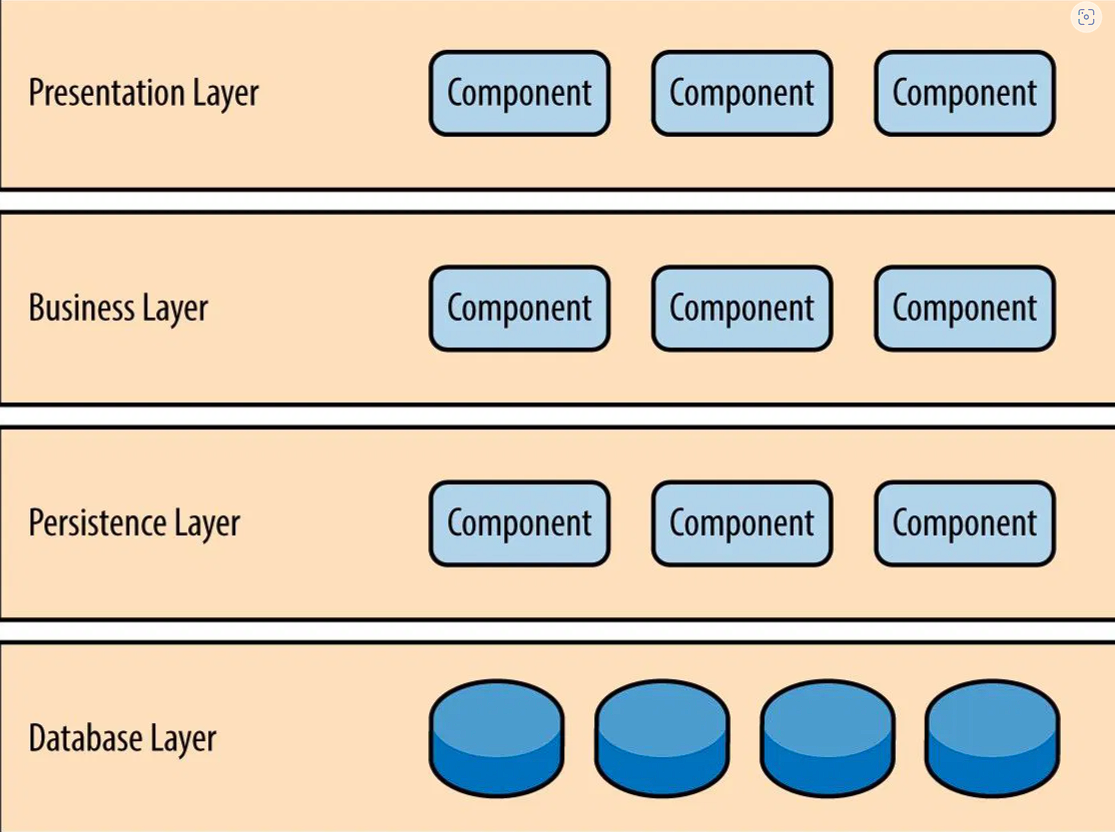
\includegraphics[scale = 0.3]{img/Layered_Architecture.png}
    \caption{Mô hình một kiến trúc phân lớp tiêu chuẩn}

\end{figure}

\begin{enumerate}
    \item \textbf{Presentation Layer:} gồm các thành phần như giao diện người dùng (UI), trình duyệt web, ứng dụng điện thoại,.... Lớp này có chức năng hiển thị thông tin và kết quả từ lớp logic của người dùng và chuyển dữ liệu của người dùng nhập vào lớp logic.
    \item \textbf{Business Layer:} Có nhiệm vụ xử lý các logic nghiệp vụ, nhận yêu cầu từ Presentation Layer, xử lý nó và gửi yêu cầu tương ứng đến Persistence Layer.
    \item \textbf{Persistence Layer:} Đảm nhiệm việc gửi các yêu cầu đến Database Layer để thực hiện các thao tác liên quan đến dữ liệu.
    \item \textbf{Database Layer:} Bao gồm cơ sở dữ liệu và các thành phần liên quan như hệ cơ sở dữ liệu. Có nhiệm vụ quản lý cơ sở dữ liệu, thực hiện thao tác đọc và ghi dữ liệu, triển khai các truy vấn và lưu trữ dữ liệu theo cách được định nghĩa từ Persistence Layer.
\end{enumerate}


\subsection{Kiến trúc hướng sự kiện (Event-driven Architecture)}

Kiến trúc hướng sự kiện là một mô hình thiết kế phần mềm tập trung vào việc tạo ra, phát hiện và phản ứng với các sự kiện. Kiến trúc hướng sự kiện bao gồm các thành phần hay dịch vụ của hệ thống giao tiếp với nhau chủ yếu thông qua việc sản xuất và tiêu thụ các sự kiện. Thay vì gọi trực tiếp đến các dịch vụ hoặc module khác, các thành phần trong hệ thống sẽ giao tiếp với nhau thông qua việc phát ra và lắng nghe các sự kiện. Các "sự kiện" này có thể là các hành động của người dùng, việc cập nhật dữ liệu hoặc các thông báo từ hệ thống khác.

Kiến trúc hướng sự kiện được phân loại dựa trên cấu trúc liên kết giữa các thành phần (component) trong hệ thống với nhau bao gồm 2 mô hình phổ biến là: Broker Topology và Mediator Topology.

\subsubsection{Quy trình làm việc của Broker Topology}

\begin{figure}[htp!]

	\centering
    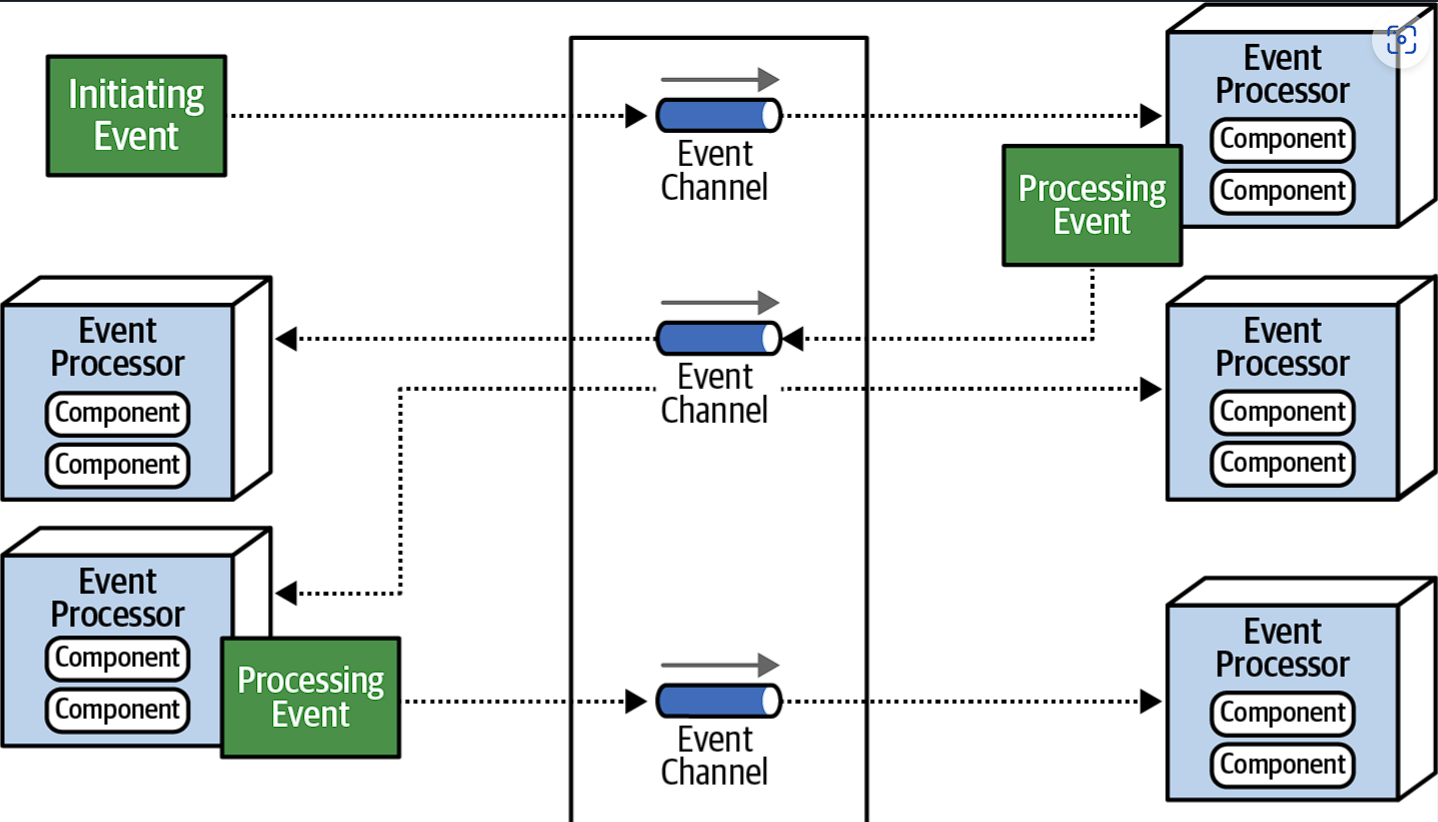
\includegraphics[scale=0.3]{img/Broker_Topology.png}
    \caption{Quy trình làm việc của Broker Topology}
\end{figure}


\subsubsection{Quy trình làm việc của Mediator Topology}

\begin{figure}[htp!]

	\centering
    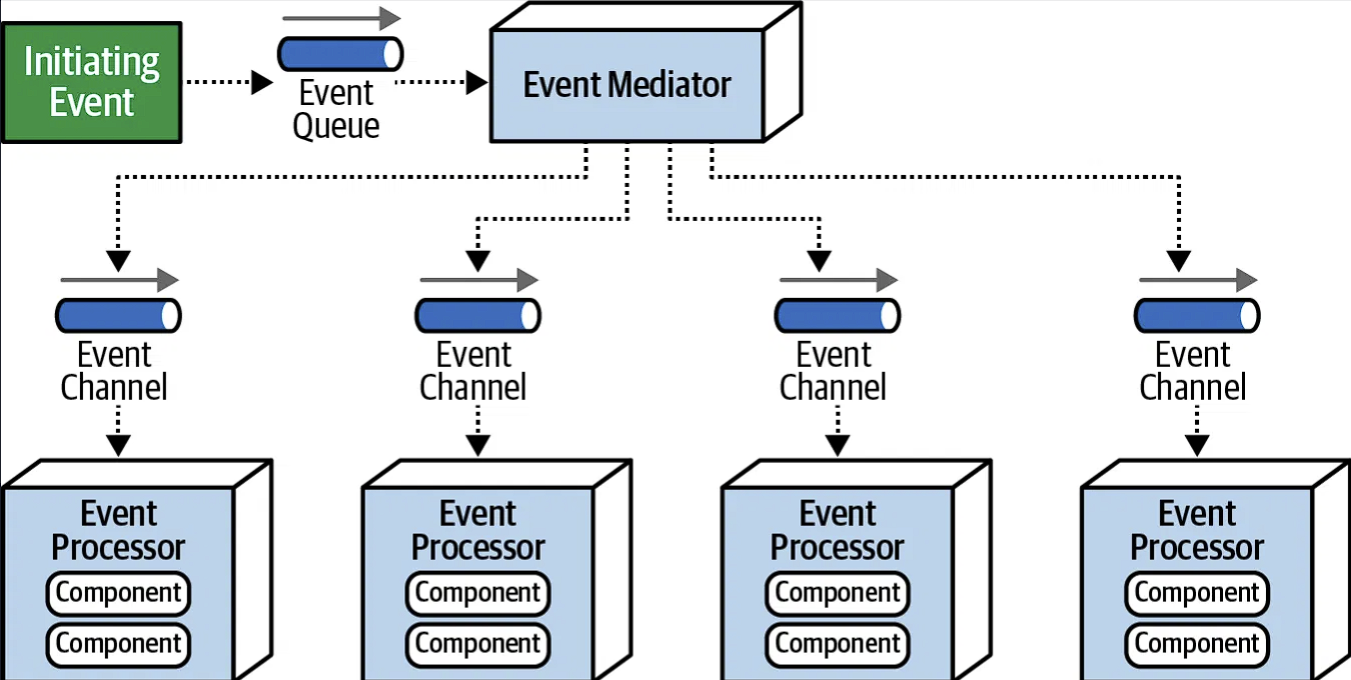
\includegraphics[scale=0.3]{img/Mediator_Topology.png}
    \caption{Quy trình làm việc của Mediator Topology}
\end{figure}


\subsection{Kiến trúc vi nhân (Microkernel Architecture)}


Kiến trúc vi nhân là một mô hình kiến trúc phần mềm, trong đó, hệ thống được phân chia thành các module hoặc các thành phần nhỏ và độc lập (được gọi là microkernel). Nó chịu trách nhiệm cho các nhiệm vụ riêng biệt như xử lý dữ liệu, lưu trữ dữ liệu,.... Kiến trúc vi nhân rất linh hoạt và dễ mở rộng, nó cho phép nhà phát triển hoặc người dùng dễ dàng thêm các chức năng và tính năng bổ sung vào ứng dụng hiện có dưới dạng tiện ích (extensions) hoặc plug-in mà không ảnh hưởng đến chức năng cốt lõi của hệ thống.


\begin{figure}[H]

	\centering
    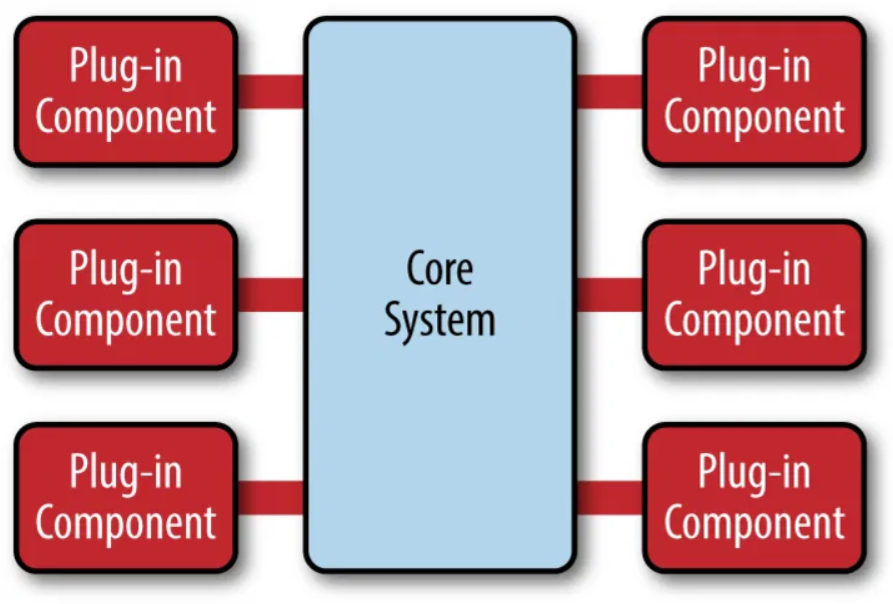
\includegraphics[scale=0.4]{img/microkernel_architecture.png}
    \caption{Cấu trúc về kiến trúc vi nhân}
\end{figure}
\newpage

Kiến trúc vi nhân bao gồm 4 thành phần chính:
\begin{itemize}
    \item \textbf{Core system (Hệ thống lõi):} bao gồm các chức năng tối thiểu cần thiết để giúp hệ thống có thể hoạt động được.
    \item \textbf{Plug-in:} bao gồm các thành phần độc lập, có khả năng xử lý chuyên biệt, có các tính năng bổ sung và mã tùy chỉnh nhằm nâng cao hoặc mở rộng hệ thống cốt lõi. Bên cạnh đó, các plug-in phải độc lập với nhau và không phụ thuộc lẫn nhau trong quá trình hoạt động.
    \item \textbf{Register:} core system sẽ dùng registry để xác định plug-in nào đang khả dụng và kết nối tới plug-in đó như thế nào.
    \item \textbf{Contract:} thể hiện mối quan hệ giữa hệ thống lõi và các mô-đun plug-in bao gồm hành vi, giao thức truy cập từ xa từ hệ thống lõi tới plug-in, dữ liệu đầu vào và đầu ra của các plug-in.
\end{itemize}

\subsection{Kiến trúc Microservice}

Kiến trúc Microservice là một phong cách kiến trúc phần mềm trong đó một ứng dụng được chia thành các dịch vụ nhỏ, độc lập, mỗi dịch vụ thực hiện một chức năng cụ thể và giao tiếp với nhau thông qua các giao diện lập trình ứng dụng (API). Các dịch vụ này có thể được phát triển, triển khai và mở rộng một cách độc lập, giúp tăng tính linh hoạt và khả năng mở rộng của hệ thống.


\begin{figure}[H]

	\centering
    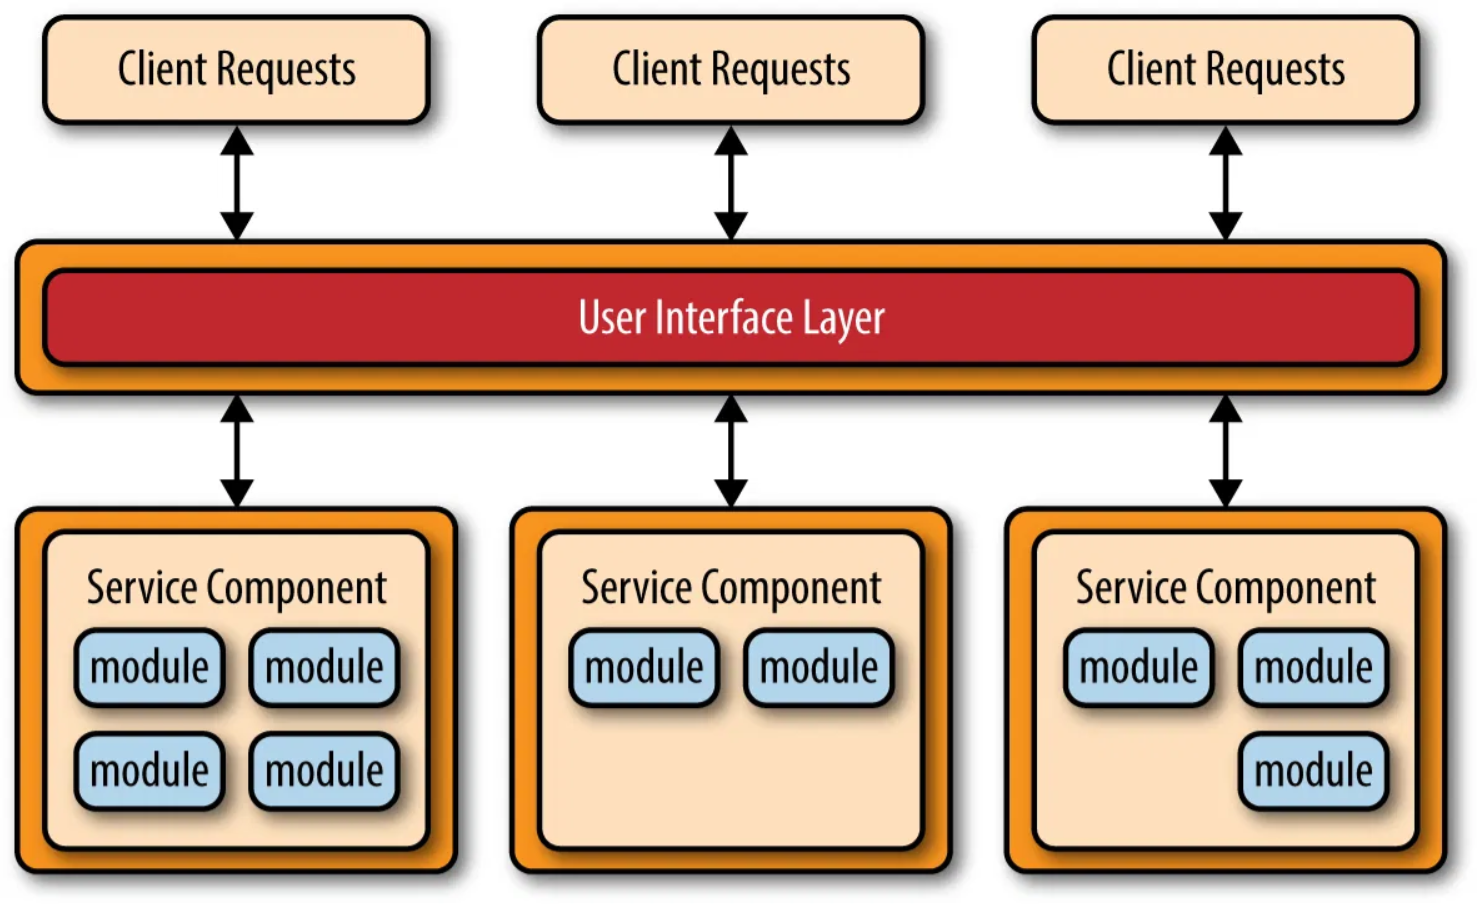
\includegraphics[scale = 0.25]{img/Microservice_Architecture.png}
    \caption{Cấu trúc về kiến trúc Microservice}
\end{figure}

Kiến trúc Microservice được xây dựng dựa trên "bounded context": Mỗi service mô hình hoá một domain hoặc một workflow. Tức là mỗi service có thể chứa mọi thứ cần thiết để hoạt động trong ứng dụng, bao gồm các class, các thành phần con trong nó và database.

Mặc dù kiến trúc Microservice rất phổ biến và mạnh mẽ nhưng đây cũng là một kiến trúc rất khó triển khai nhất. 

\subsection{Mô hình MVCs (Model - View - Controller)}

Mô hình MVCs là một mẫu kiến trúc, mô hình lập trình phổ biến được sử dụng để tạo cấu trúc cho nhiều trang web, ứng dụng tiên tiến.

MVCs được chia làm 3 phần phụ thuộc và kết nối với nhau:
\begin{itemize}
    \item \textbf{Model:} có vai trò quản lý dữ liệu và logic nghiệp vụ của ứng dụng. Nó giúp xử lý dữ liệu, tương tác với cơ sở dữ liệu và thực hiện các thao tác nghiệp vụ.
    \item \textbf{View:} là thành phần hiển thị dữ liệu và giao diện người dùng, giúp người xem có thể xem được thông tin trang web và ứng dụng một cách trực quan. Nó nhận ữ liệu từ Model và hiển thị cho người dùng, nhận các tương tác từ người dùng và chuyển tiếp đến Controller.
    \item \textbf{Controller:} có chức năng nhận các yêu cầu từ View, gọi các phương thức từ Model để xử lý dữ liệu và cập nhật View. Nó vai trò điều khiển luồng dữ liệu giữa Model và View.
\end{itemize}

\begin{figure}[H]

	\centering
    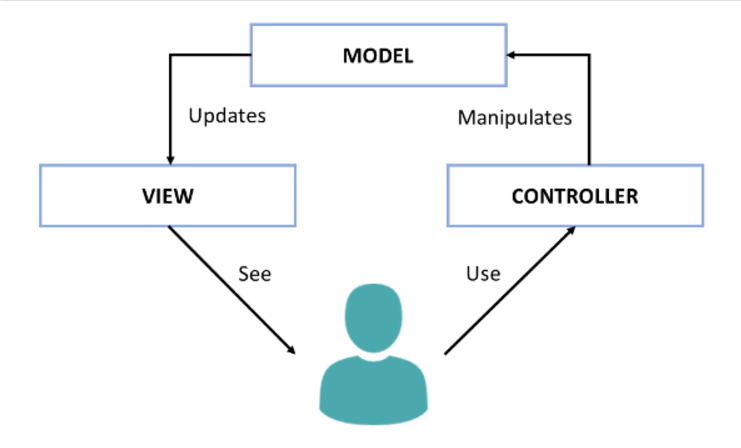
\includegraphics[scale=0.4]{img/MVCs_workflow.png}
    \caption{Quy trình làm việc của mô hình MVCs}
\end{figure}

Khi bạn gửi những yêu cầu, request đến Controller và Controller nhận được yêu cầu từ người dùng, chúng sẽ kiểm tra yêu cầu có cần lấy dữ liệu từ Model hay không. Nếu cần Controller sẽ dùng các class/function sẵn có để trả kết quả. Sau khi xử lý các dữ liệu đó, nó sẽ trả qua View để hiển thị.

Còn View sẽ chịu trách nhiệm cho phần hiển thị như thống tin dữ liệu, hình ảnh,.... Rồi trả về GUI Content để Controller đưa kết quả lên Browser. Trình duyệt sẽ tiếp nhận dữ liệu và trả lại kết quả tìm kiếm cho người dùng.

\subsection{Thiết kế kiến trúc hệ thống}

Ở đồ án này tôi sử dụng mô hình kiến trúc MVCs vì những lợi ích trong việc phát triển phần mềm, đặc biệt trong các ứng dụng giao diện người dùng. Nó cho phép các lập trình viên phân tách rõ ràng cấu trúc model, data, giao diện người dùng và nghiệp vụ. MVCs cũng cung cấp đa dạng hình thức View cho nhiều đối tượng khác nhau. Thậm chí, ta có thể tái sử dụng các Model hay View mà không bị ảnh hưởng tới các thành phần khác. Do bởi Controller và Model độc lập với View, nên nó giúp cho hệ thống dễ dàng mở rộng và kiểm thử hơn.

\subsubsection{Dưới đây là sự so sánh MVCs với các kiến trúc khác:}


\begin{table}[H]
    \centering
    \begin{tabular}{|>{\centering\arraybackslash}p{0.1\linewidth}|>{\centering\arraybackslash}p{0.15\linewidth}|>{\centering\arraybackslash}p{0.15\linewidth}|>{\centering\arraybackslash}p{0.15\linewidth}|>{\centering\arraybackslash}p{0.13\linewidth}|>{\centering\arraybackslash}p{0.13\linewidth}|} \hline 
         Tiêu chí&  MVCs&  Layered Architecture&   Microservices Architecture&  Microkernel Architecture& Event-driven Architecture\\ \hline 
         Mục tiêu thiết kế&  Tách rõ ràng giữa Model, View, Controller&  Tách biệt các tầng (layer) theo chức năng logic&  Tách biệt theo dịch vụ độc lập&  Tách biệt giữa kernel (cốt lõi) và các plugin& Tách biệt thành phần sản xuất \& xử lý sự kiện\\ \hline 
         Khả năng mở rộng&  Phù hợp cho ứng dụng vừa và nhỏ. Khó mở rộng khi hệ thống quá phức tạp.&  Dễ mở rộng theo chiều dọc nhưng khó mở rộng theo chiều ngang (tầng thường bị phụ thuộc lẫn nhau).&  Rất cao (dịch vụ độc lập)&  Cao (thêm plugin hoặc mở rộng kernel)& Cao (có thể thêm nhiều producer hoặc consumer)\\ \hline 
         Tính linh hoạt&  Tốt, nhưng Controller thường phụ thuộc vào logic business&  Trung bình (thay đổi 1 tầng có thể ảnh hưởng tầng khác)&  Cao, nhưng phức tạp hơn trong việc phối hợp&  Trung bình (phụ thuộc vào cốt lõi kernel)& Cao, nhưng khó quản lý các sự kiện phức tạp\\ \hline 
         Độ phức tạp khi triển khai&  Đơn giản, dễ hiểu. Thích hợp cho ứng dụng nhỏ và trung bình.&  Đơn giản trong hệ thống nhỏ, nhưng phức tạp dần khi có nhiều tầng phụ thuộc lẫn nhau.&  Phức tạp cao, yêu cầu quản lý giao tiếp giữa các service.&  Đơn giản khi thiết kế lõi, nhưng phức tạp hơn khi thêm plugin.& Phức tạp khi xử lý đồng bộ nhiều sự kiện và quản lý message broker.\\ \hline 
         Khả năng tái sử dụng&  Cao ở Model và View.&  Cao ở các tầng logic.&  Cao (để chia sẻ hoặc sử dụng lại các dịch vụ)&  Cao (plugin để tái sử dụng)& Thấp nếu không chuẩn hóa sự kiện\\ \hline 
         Dễ bảo trì&  Dễ bảo trì với các ứng dụng nhỏ, khó bảo trì khi mở rộng hệ thống phức tạp.&  Dễ bảo trì với cấu trúc phân tầng rõ ràng, nhưng phụ thuộc lẫn nhau có thể gây khó khăn.&  Dễ bảo trì nhờ tính độc lập của từng microservice, nhưng cần chú ý sự đồng nhất trong các giao diện API.&  Dễ bảo trì, plugin có thể thay thế hoặc nâng cấp mà không ảnh hưởng lõi.& Phụ thuộc vào cách tổ chức các sự kiện và logic xử lý.\\ \hline
    \end{tabular}
    \caption{So sánh MVCs với các kiến trúc khác}
    \label{tab:MVCs_comparasion}
\end{table}

Chính vì các lý do trên, nên tôi đã sử dụng kiến túc MVCs trong quá trình thiết kế kiến trúc hệ thống của trang web. Hình dưới đã minh hoạ tổng quan và khái quát cách tôi sẽ triển khai hệ thống của mình. Sẽ có 4 View cho 4 đối tượng khác nhau gồm: User/Applicant, Admin, Recruiter/Company và external stakeholder. Với những đối tượng như User/Applicant, Admin, Recruiter/Company, họ cần phải đăng nhập vào trang web để có View của mình. Còn đối với External Stakeholder, họ là đối tượng không cần đăng nhập nhưng vẫn có thể quan sát được trang web với một View riêng. Về Front-end, sẽ được thiết kế và triển khai bằng ngôn ngữ ReactJS. Front-end sẽ được kết nối với back-end - sử dụng MongoDB thông qua HTTPS. Các dữ liệu của back-end cũng sẽ được lưu giữ trong cơ sở dữ liệu của MongoDB.

\subsubsection{Thiết kế kiến trúc hệ thống}

\begin{figure}[H]

	\centering
    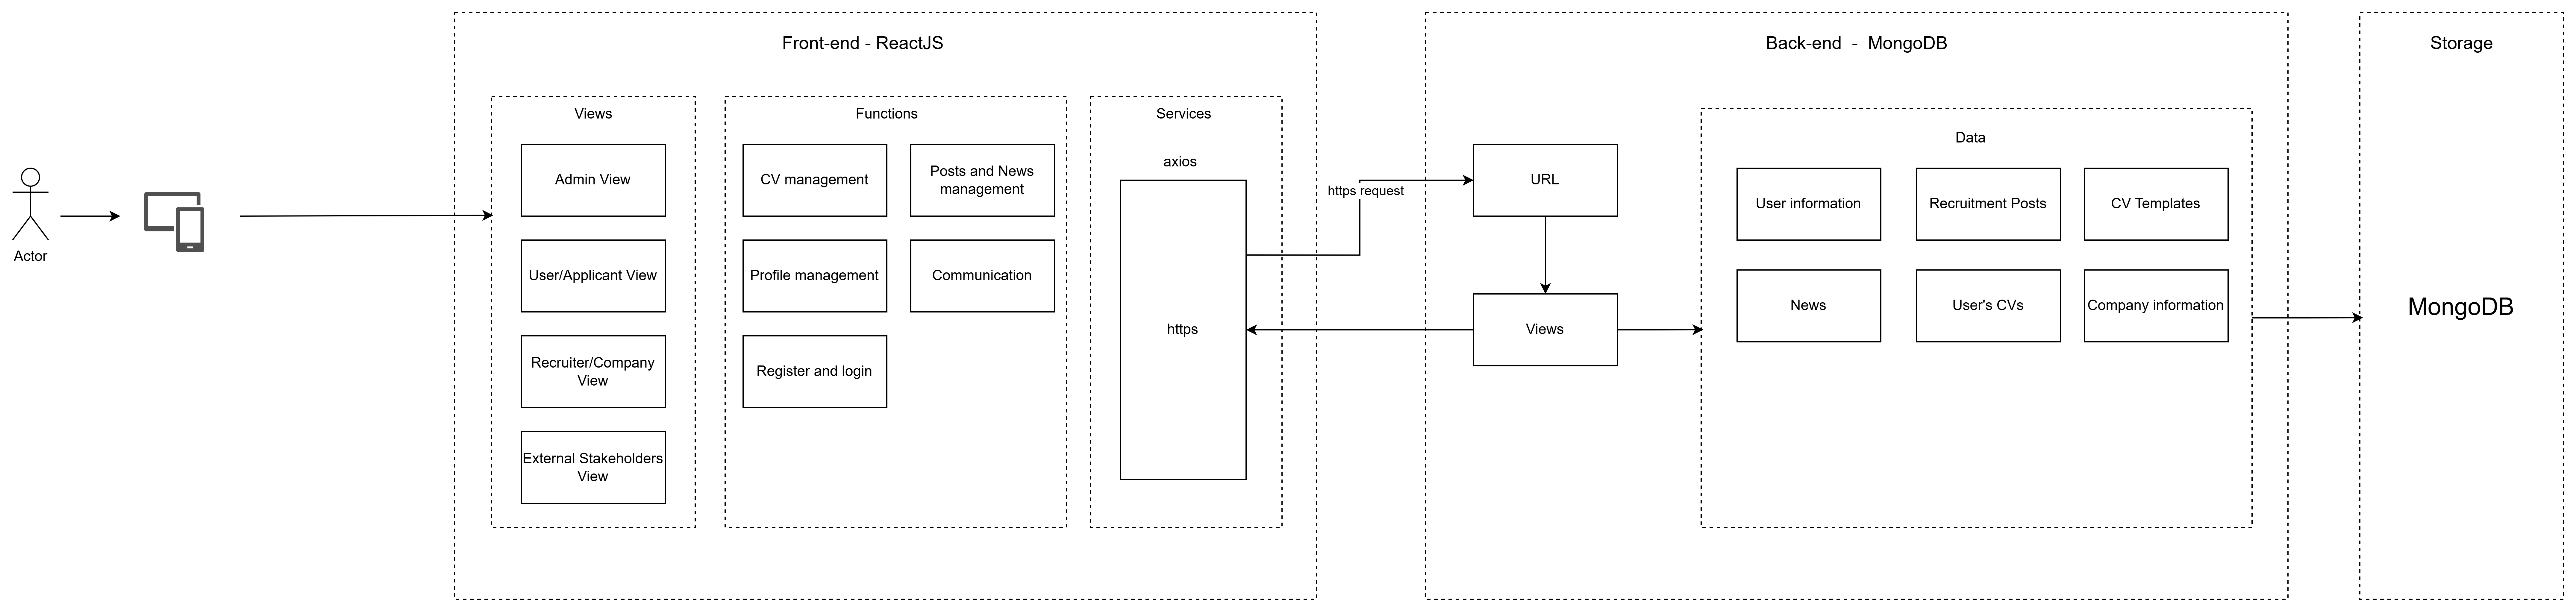
\includegraphics[angle=90,scale=0.07]{img/system_architecture.png}
    \caption{Kiến trúc hệ thống của trang web}
\end{figure}




\section{Lược đồ lớp (Class diagram)}

\subsection{Khái quát về class diagram}

Class Diagram là một loại biểu đồ trong kỹ thuật phần mềm, được sử dụng để mô tả cấu trúc và mối quan hệ giữa các lớp trong một hệ thống phần mềm. Nó là một phần quan trọng của mô hình hóa phân cấp, hay còn được gọi là UML (Unified Modeling Language), được sử dụng rộng rãi trong việc phát triển phần mềm.

Class diagram (biểu đồ lớp) đóng vai trò thiết yếu trong việc mô hình hóa cấu trúc của các hệ thống phần mềm. Nó giúp các nhà phát triển phần mềm có cái nhìn tổng quan về kiến trúc của hệ thống. Nó cung cấp thông tin chi tiết về cách các đối tượng trong hệ thống tương tác với nhau, từ đó hỗ trợ việc lập kế hoạch, thiết kế và triển khai một cách hiệu quả.




\subsection{Thiết kế lược đồ lớp}

\begin{figure}[H]

	\centering
    \includegraphics[angle = 90,scale=0.05]{img/ClassDiagram.png}
    \caption{Lược lớp của hệ thống}
\end{figure}




\subsection{Lớp điều khiển (Controller Layer)}

\begin{figure}[H]

	\centering
    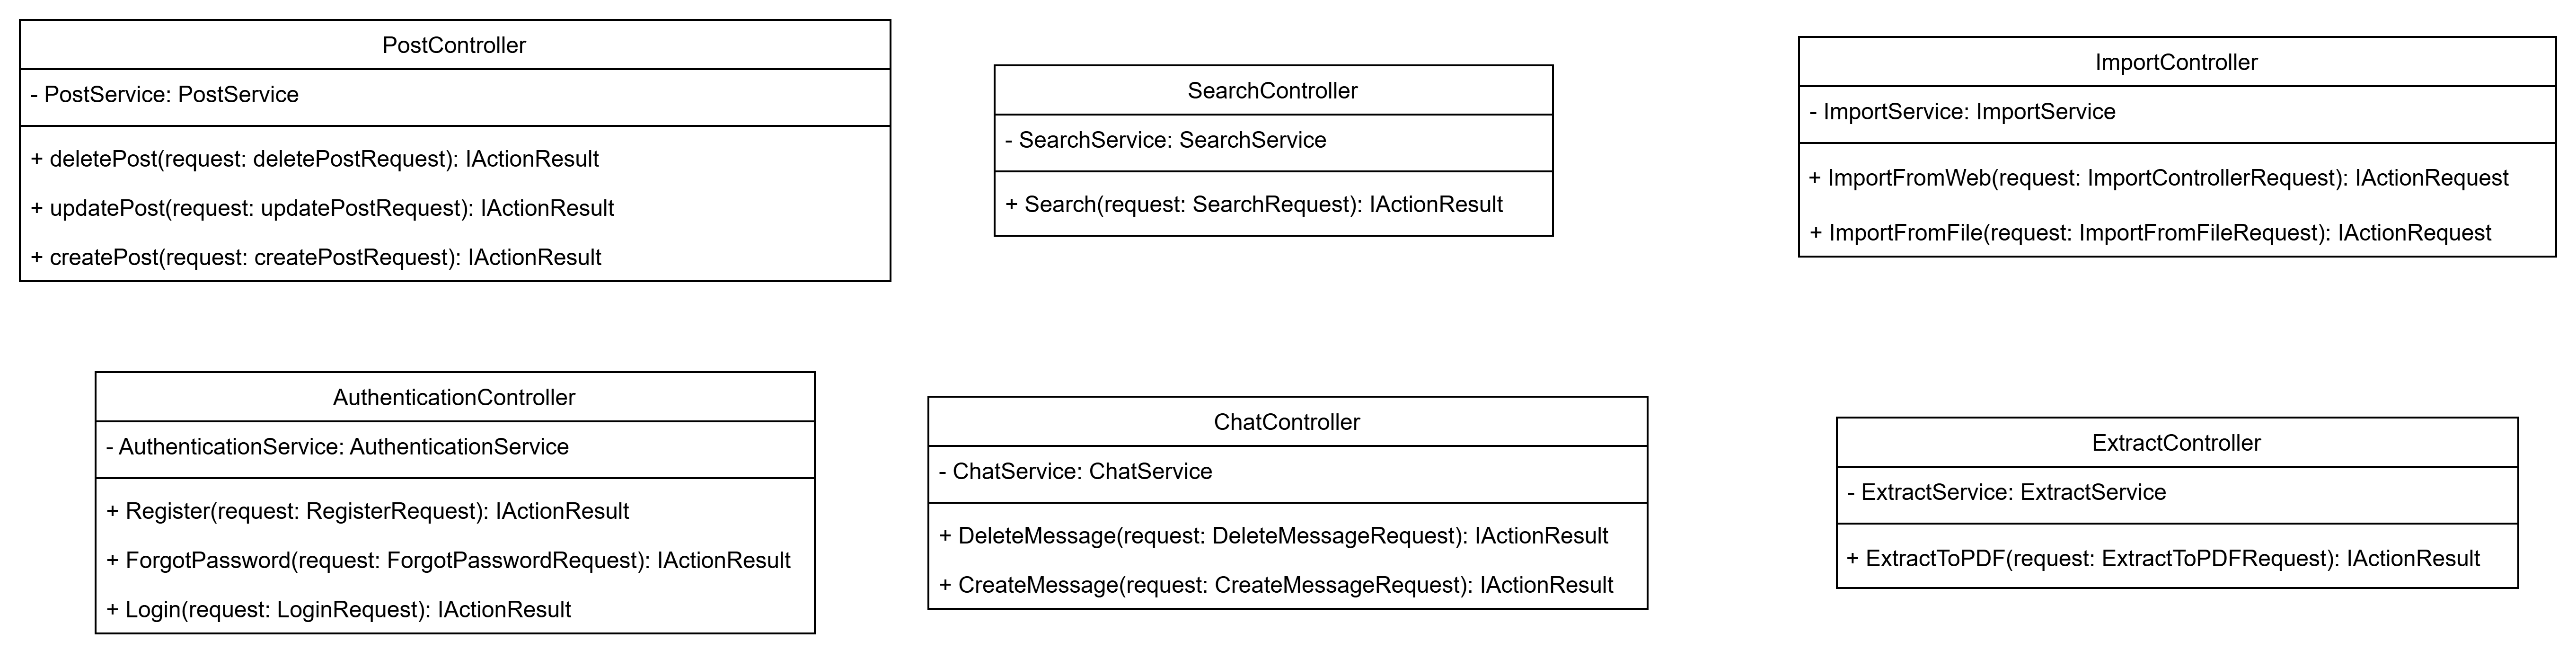
\includegraphics[scale=0.08]{img/Controller_view.png}
    \caption{Lớp điều khiển của lược đồ lớp}
\end{figure}

Lớp điều khiển (Controller Layer) là lớp chịu trách nhiệm cho việc tiếp nhận yêu cầu từ hành động cụ thể của người dùng lên giao diện của trang web và gửi lại phản hồi cho người dùng. Hệ thống sẽ tiếp nhận yêu cầu của người dùng, gọi các dịch vụ từ lớp dịch vụ, xử lý và phản hồi yêu cầu của người dùng thông qua hiển thị thông báo lên trang web.


\subsection{Lớp dịch vụ (Service Layer) }

\begin{figure}[H]

	\centering
    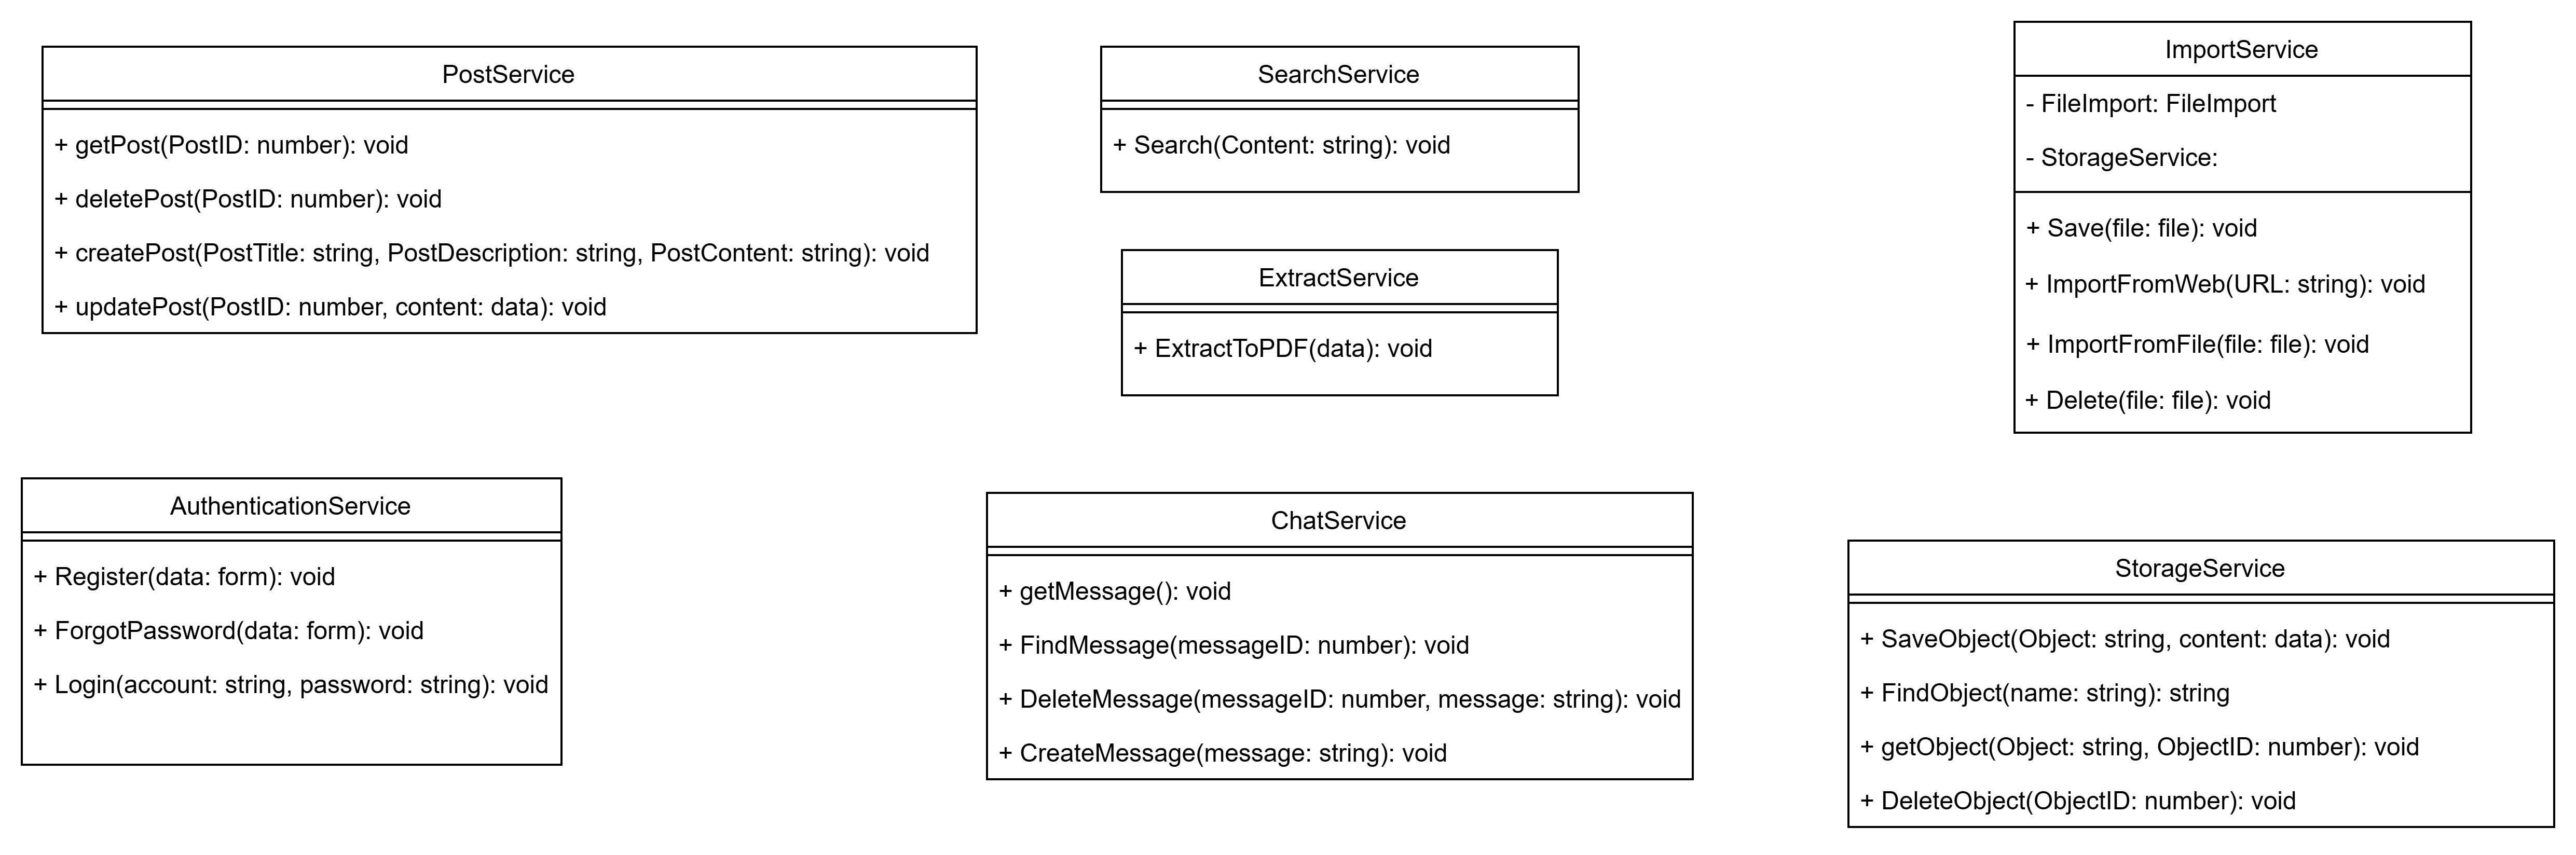
\includegraphics[scale=0.06]{img/Service_layer.png}
    \caption{Lớp dịch vụ của lược đồ lớp}
\end{figure}

Lớp dịch vụ (Service Layer) là lớp trung gian giữa controller và model. Nó chứa toàn bộ logic nghiệp vụ (business logic) của ứng dụng. Nó giúp xử lý yêu cầu từ lớp Controller và giao tiếp với lớp dữ liệu (Model Layer)  để truy xuất dữ liệu.


\subsection{Lớp dữ liệu (Model Layer)}

\begin{figure}[H]

	\centering
    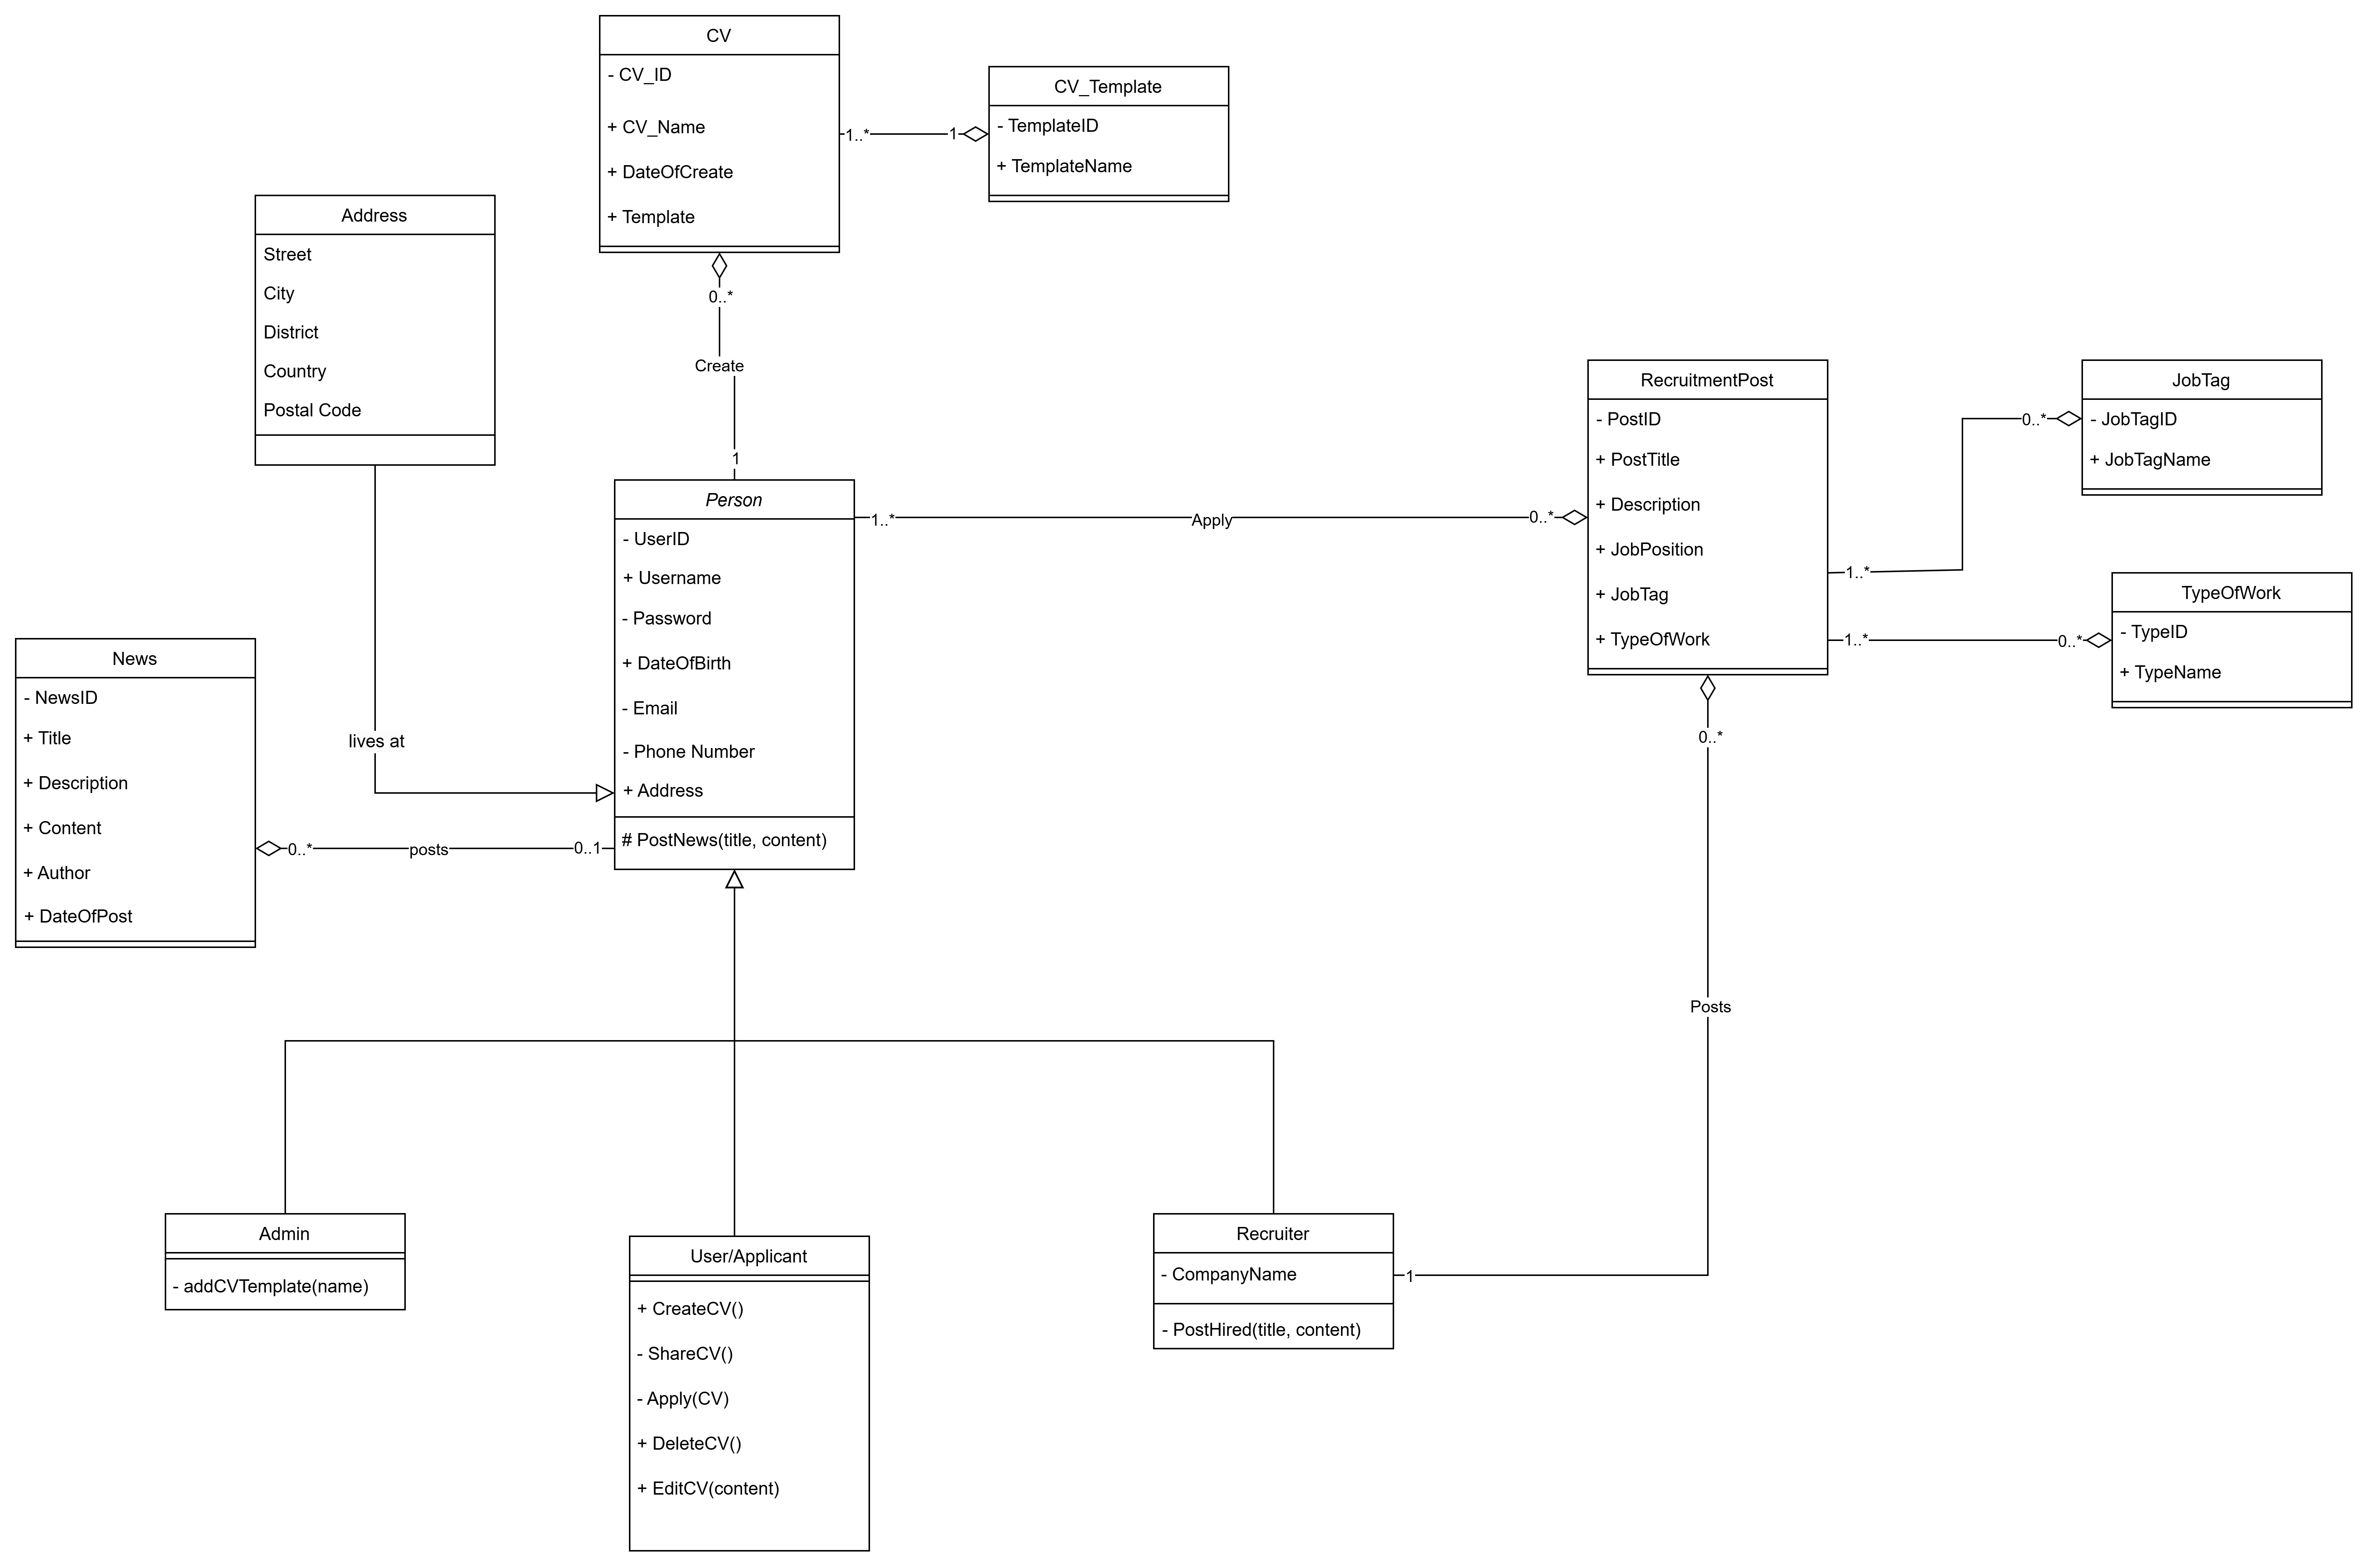
\includegraphics[scale=0.07]{img/Overview_classDiagram.png}
    \caption{Lớp dữ liệu của lược đồ lớp}

	
\end{figure}

Lớp dữ liệu (Model Layer) là lớp chứa các đối tượng mô hình hóa dữ liệu trong hệ thống. Các class trong Model Layer đại diện cho các thực thể trong cơ sở dữ liệu bao gồm các thực thể: news, user, CV, CV template, recruitementPost, JobTag, TypeOfWork. Toàn bộ dữ liệu của các thực thể trong lớp dữ liệu đều được lưu trữ trong StorageService.

\section{Lược đồ tuần tự (Sequence diagram)}


\subsection{Đăng ký tài khoản}

\begin{figure}[H]

	\centering
    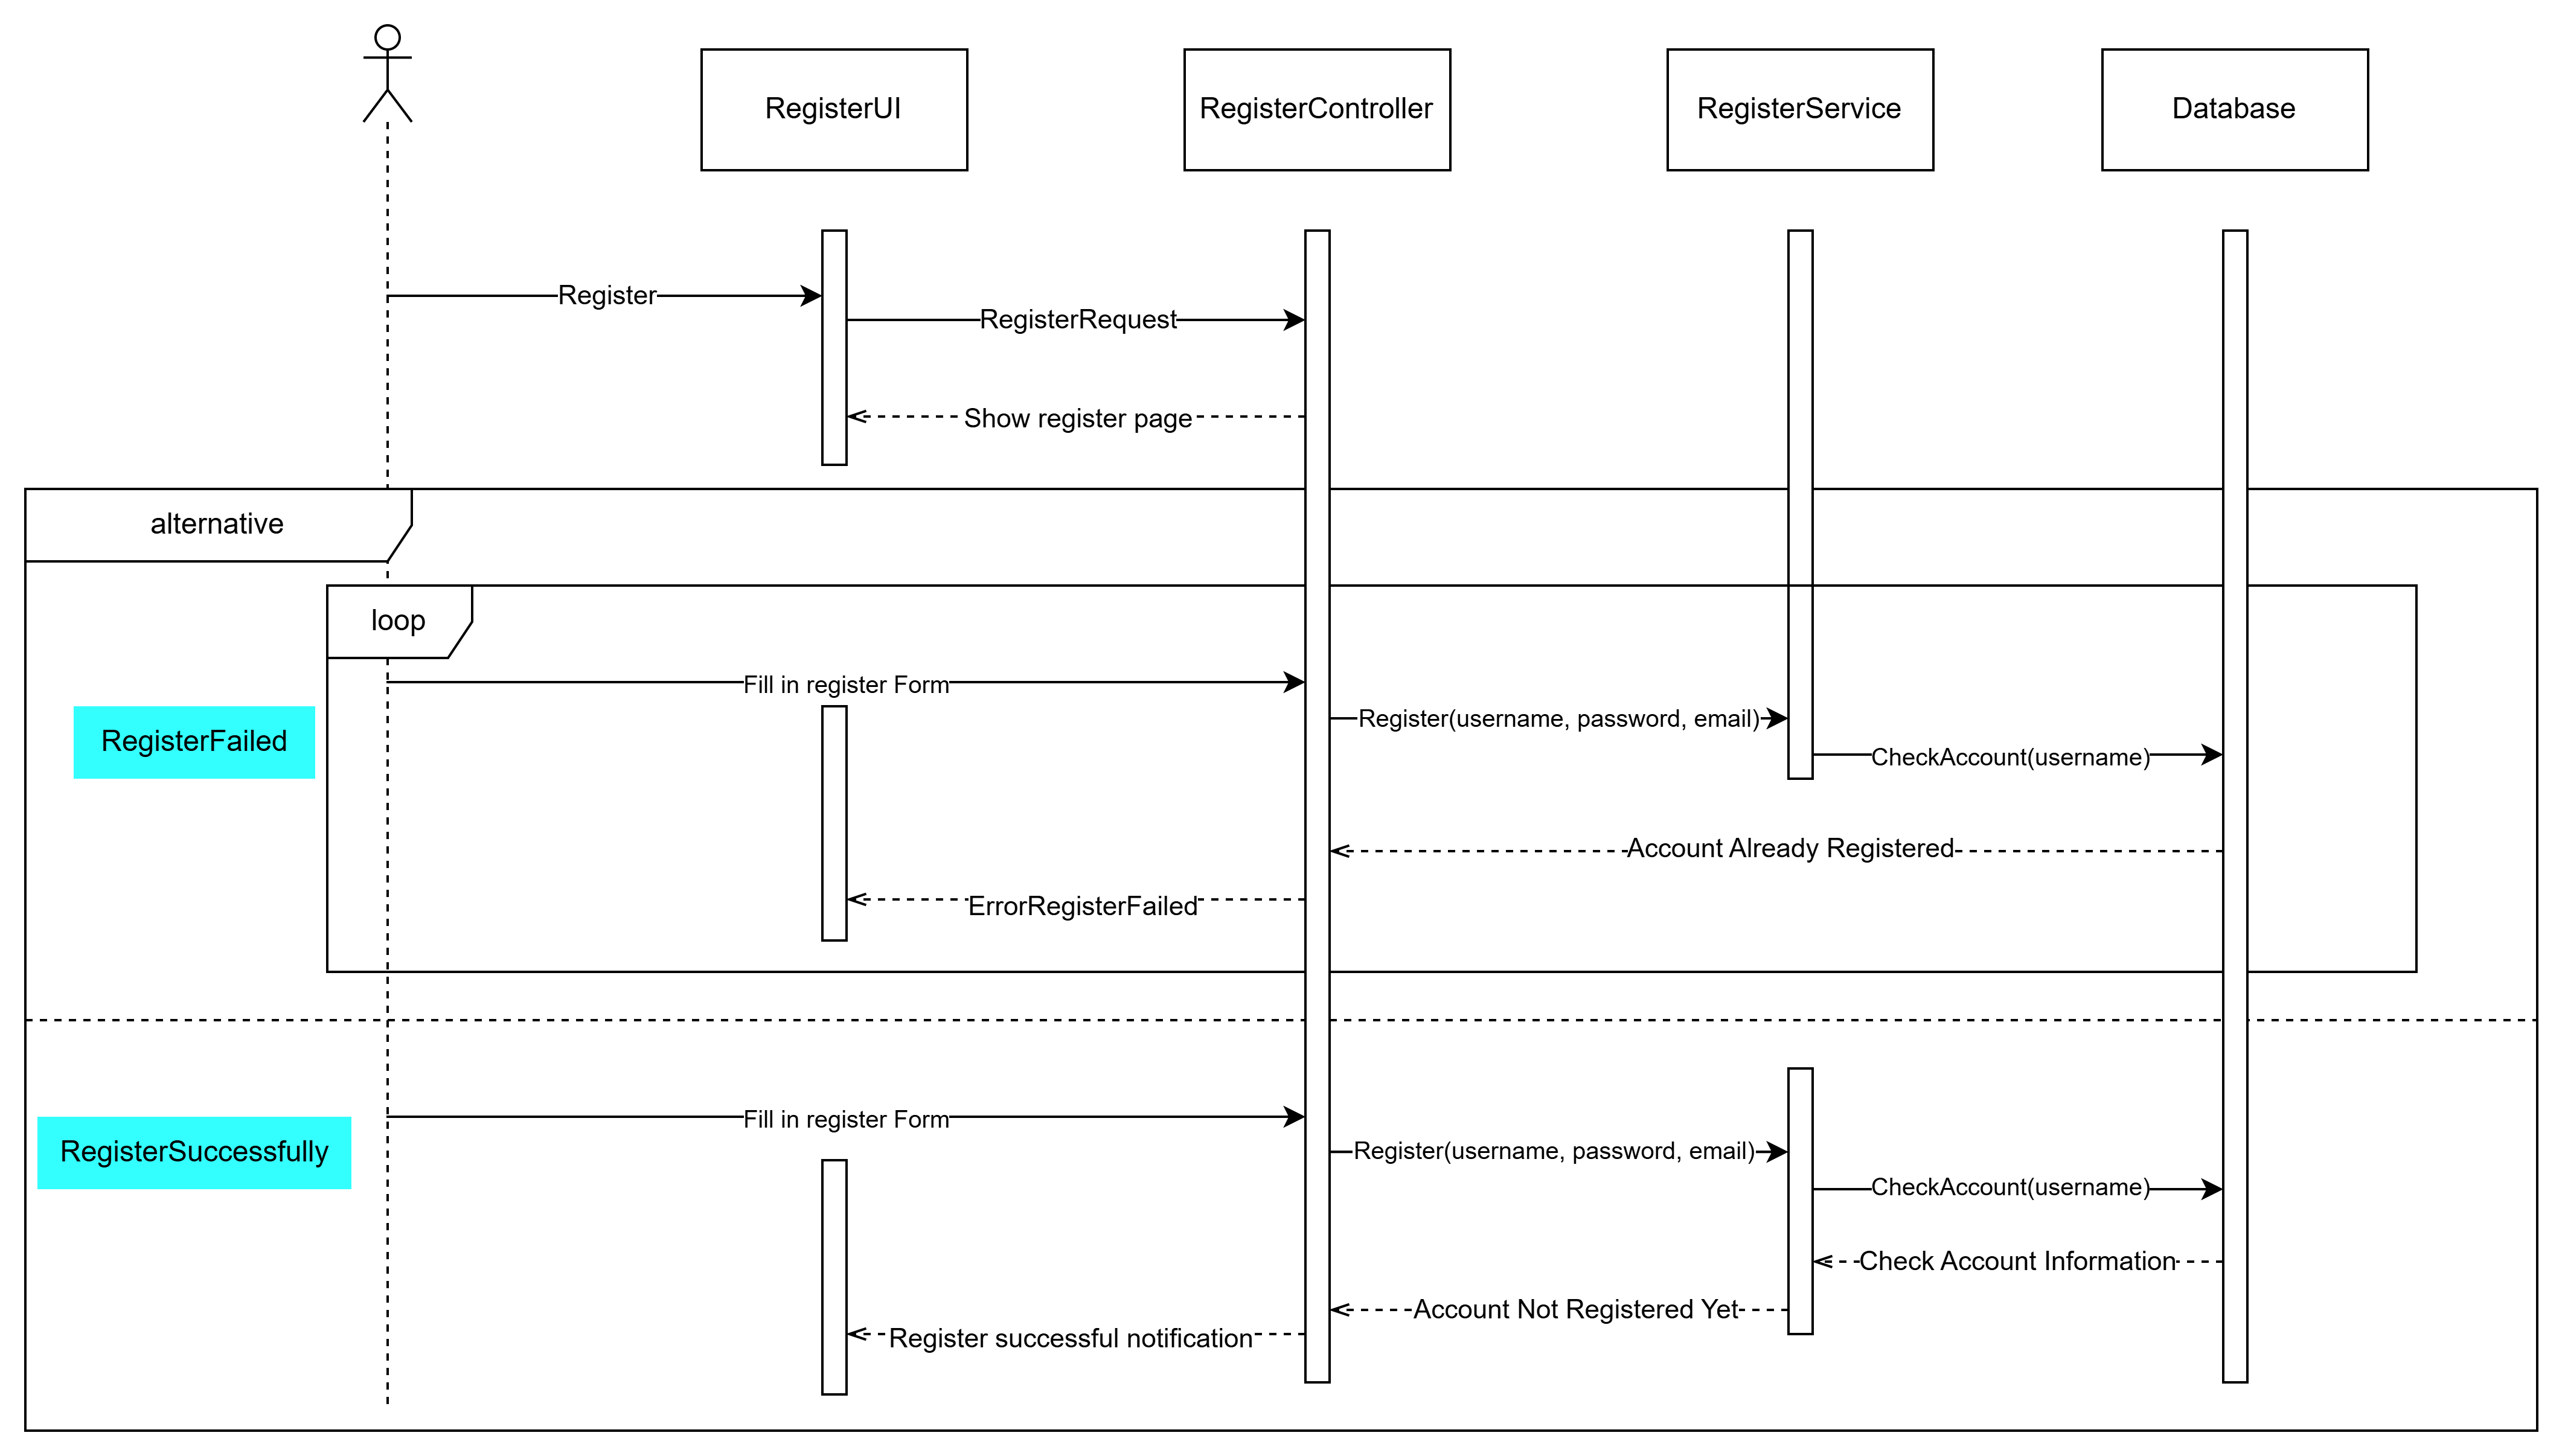
\includegraphics[scale=0.1]{img/Register_sequenceDiagram.png}
    \caption{Lược đồ tuần tự cho Đăng ký tài khoản}
	
\end{figure}

Khi người dùng chọn "Đăng ký tài khoản", người dùng sẽ được đưa đến trang "Đăng ký tài khoản". Ở đó sẽ chứa biểu mẫu yêu cầu người dùng điền vào để có thể tạo tài khoản thành công. Sau khi hoàn thành công việc điền biểu mẫu và yêu cầu tạo tài khoản, hệ thống sẽ kiểm tra thông tin tài khoản người dùng đã có trong cơ sở dữ liệu của hệ thống chưa? Nếu chưa có, hệ thống sẽ tạo tài khoản thành công, thông báo cho người dùng "Tạo tài khoản thành công" và chuyển hướng người dùng đến trang "Đăng nhập". Còn nếu tên tài khoản của người dùng đã có trong cơ sở dữ liệu, hệ thống sẽ thông báo cho người dùng "Tên tài khoản đã được sử dụng." và yêu cầu người dùng đổi tên tài khoản khác.

\subsection{Đăng nhập tài khoản }

\begin{figure}[H]

	\centering
    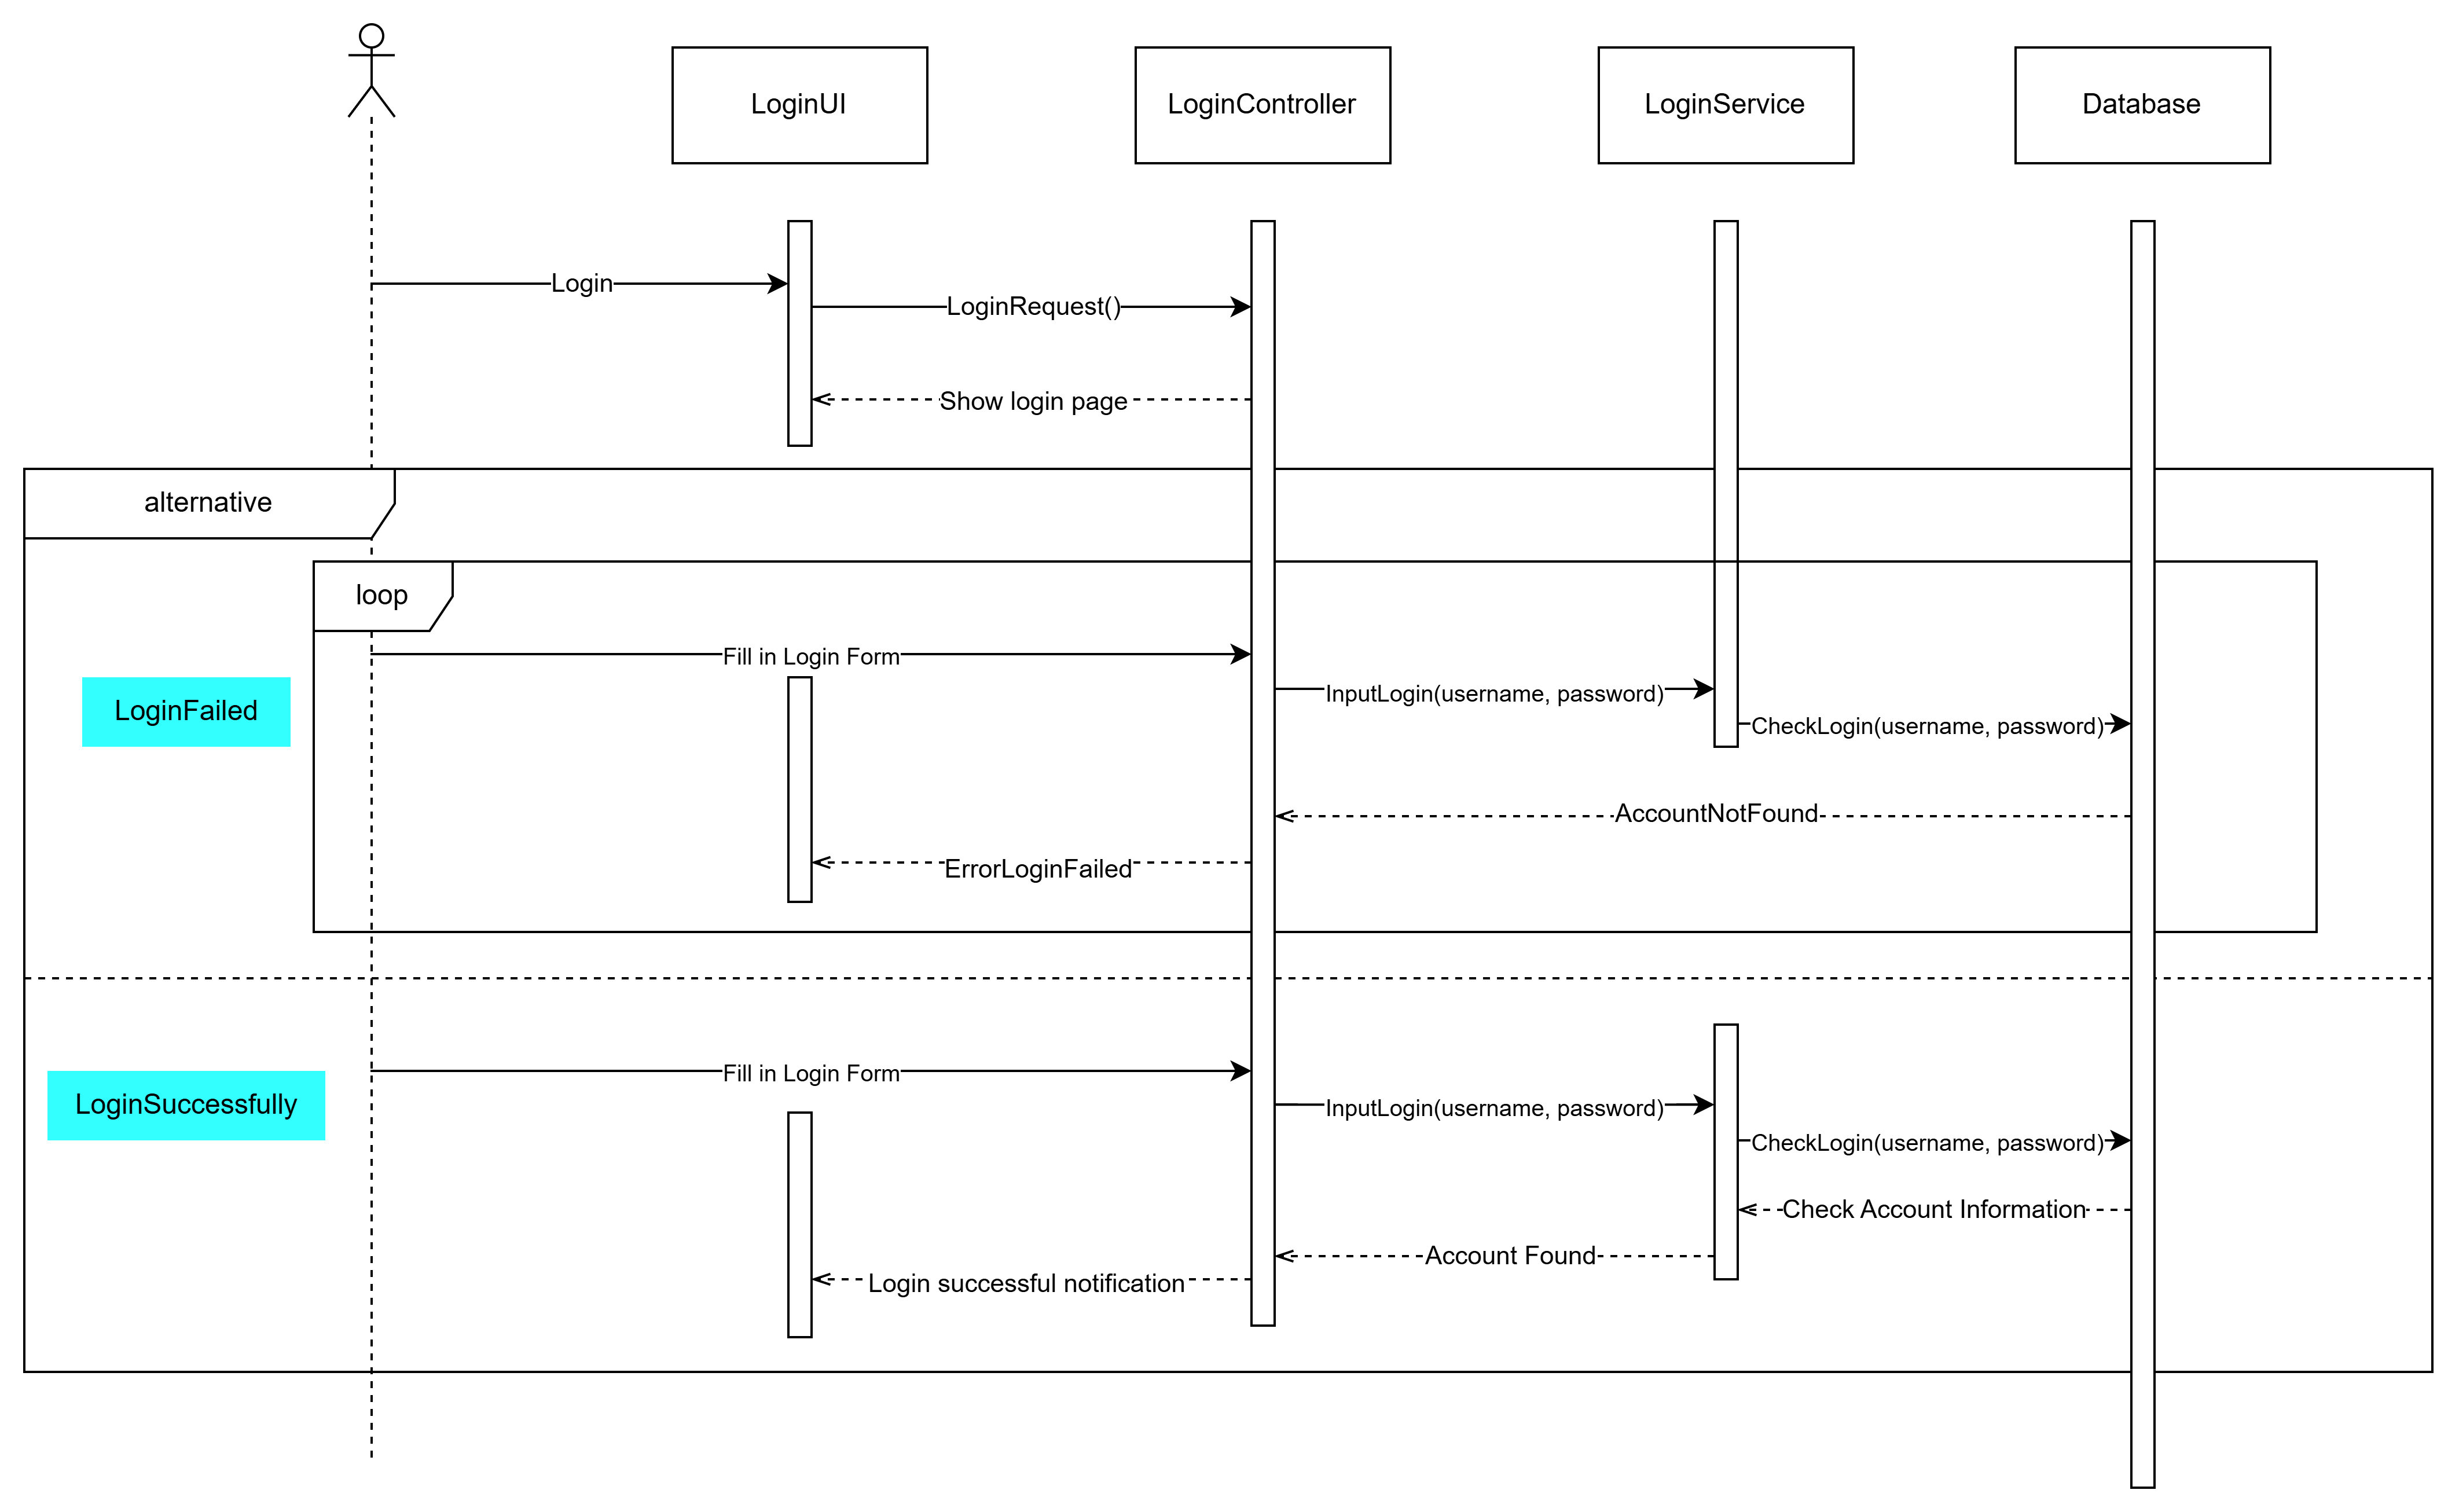
\includegraphics[scale=0.1]{img/Login_sequenceDiagram.png}
    \caption{Lược đồ tuần tự cho Đăng nhập tài khoản}
	
\end{figure}

Sơ đồ thể hiện cho quá trình đăng nhập tài khoản chung đối với nhiều vai trò người dùng khác nhau. Trong quá trình này, khi người dùng chọn phần "Đăng nhập", hệ thống sẽ chuyển hướng người dùng đến đường link của trang "Đăng nhập tài khoản". Trang web sẽ hiển thị một trang biểu mẫu cho người dùng điền tài khoản và mật khẩu. 

Sau khi người dùng điền thông tin tài khoản và mật khẩu vào biểu mẫu. Hệ thống sẽ kiểm tra thông tin tài khoản và mật khẩu mà người dùng điền vào có khớp với dữ liệu của hệ thống không? Nếu khớp, hệ thống sẽ thông báo người dùng đăng nhập thành công và chuyển hướng người dùng đến trang chủ. Nếu không khớp với dữ liệu của hệ thống, hệ thống sẽ thông báo cho người dùng "Đăng nhập thất bại" và chỉ người dùng tài khoản hay mật khẩu của người dùng bị sai.

\subsection{Quản lý CV}


\begin{figure}[H]

	\centering
    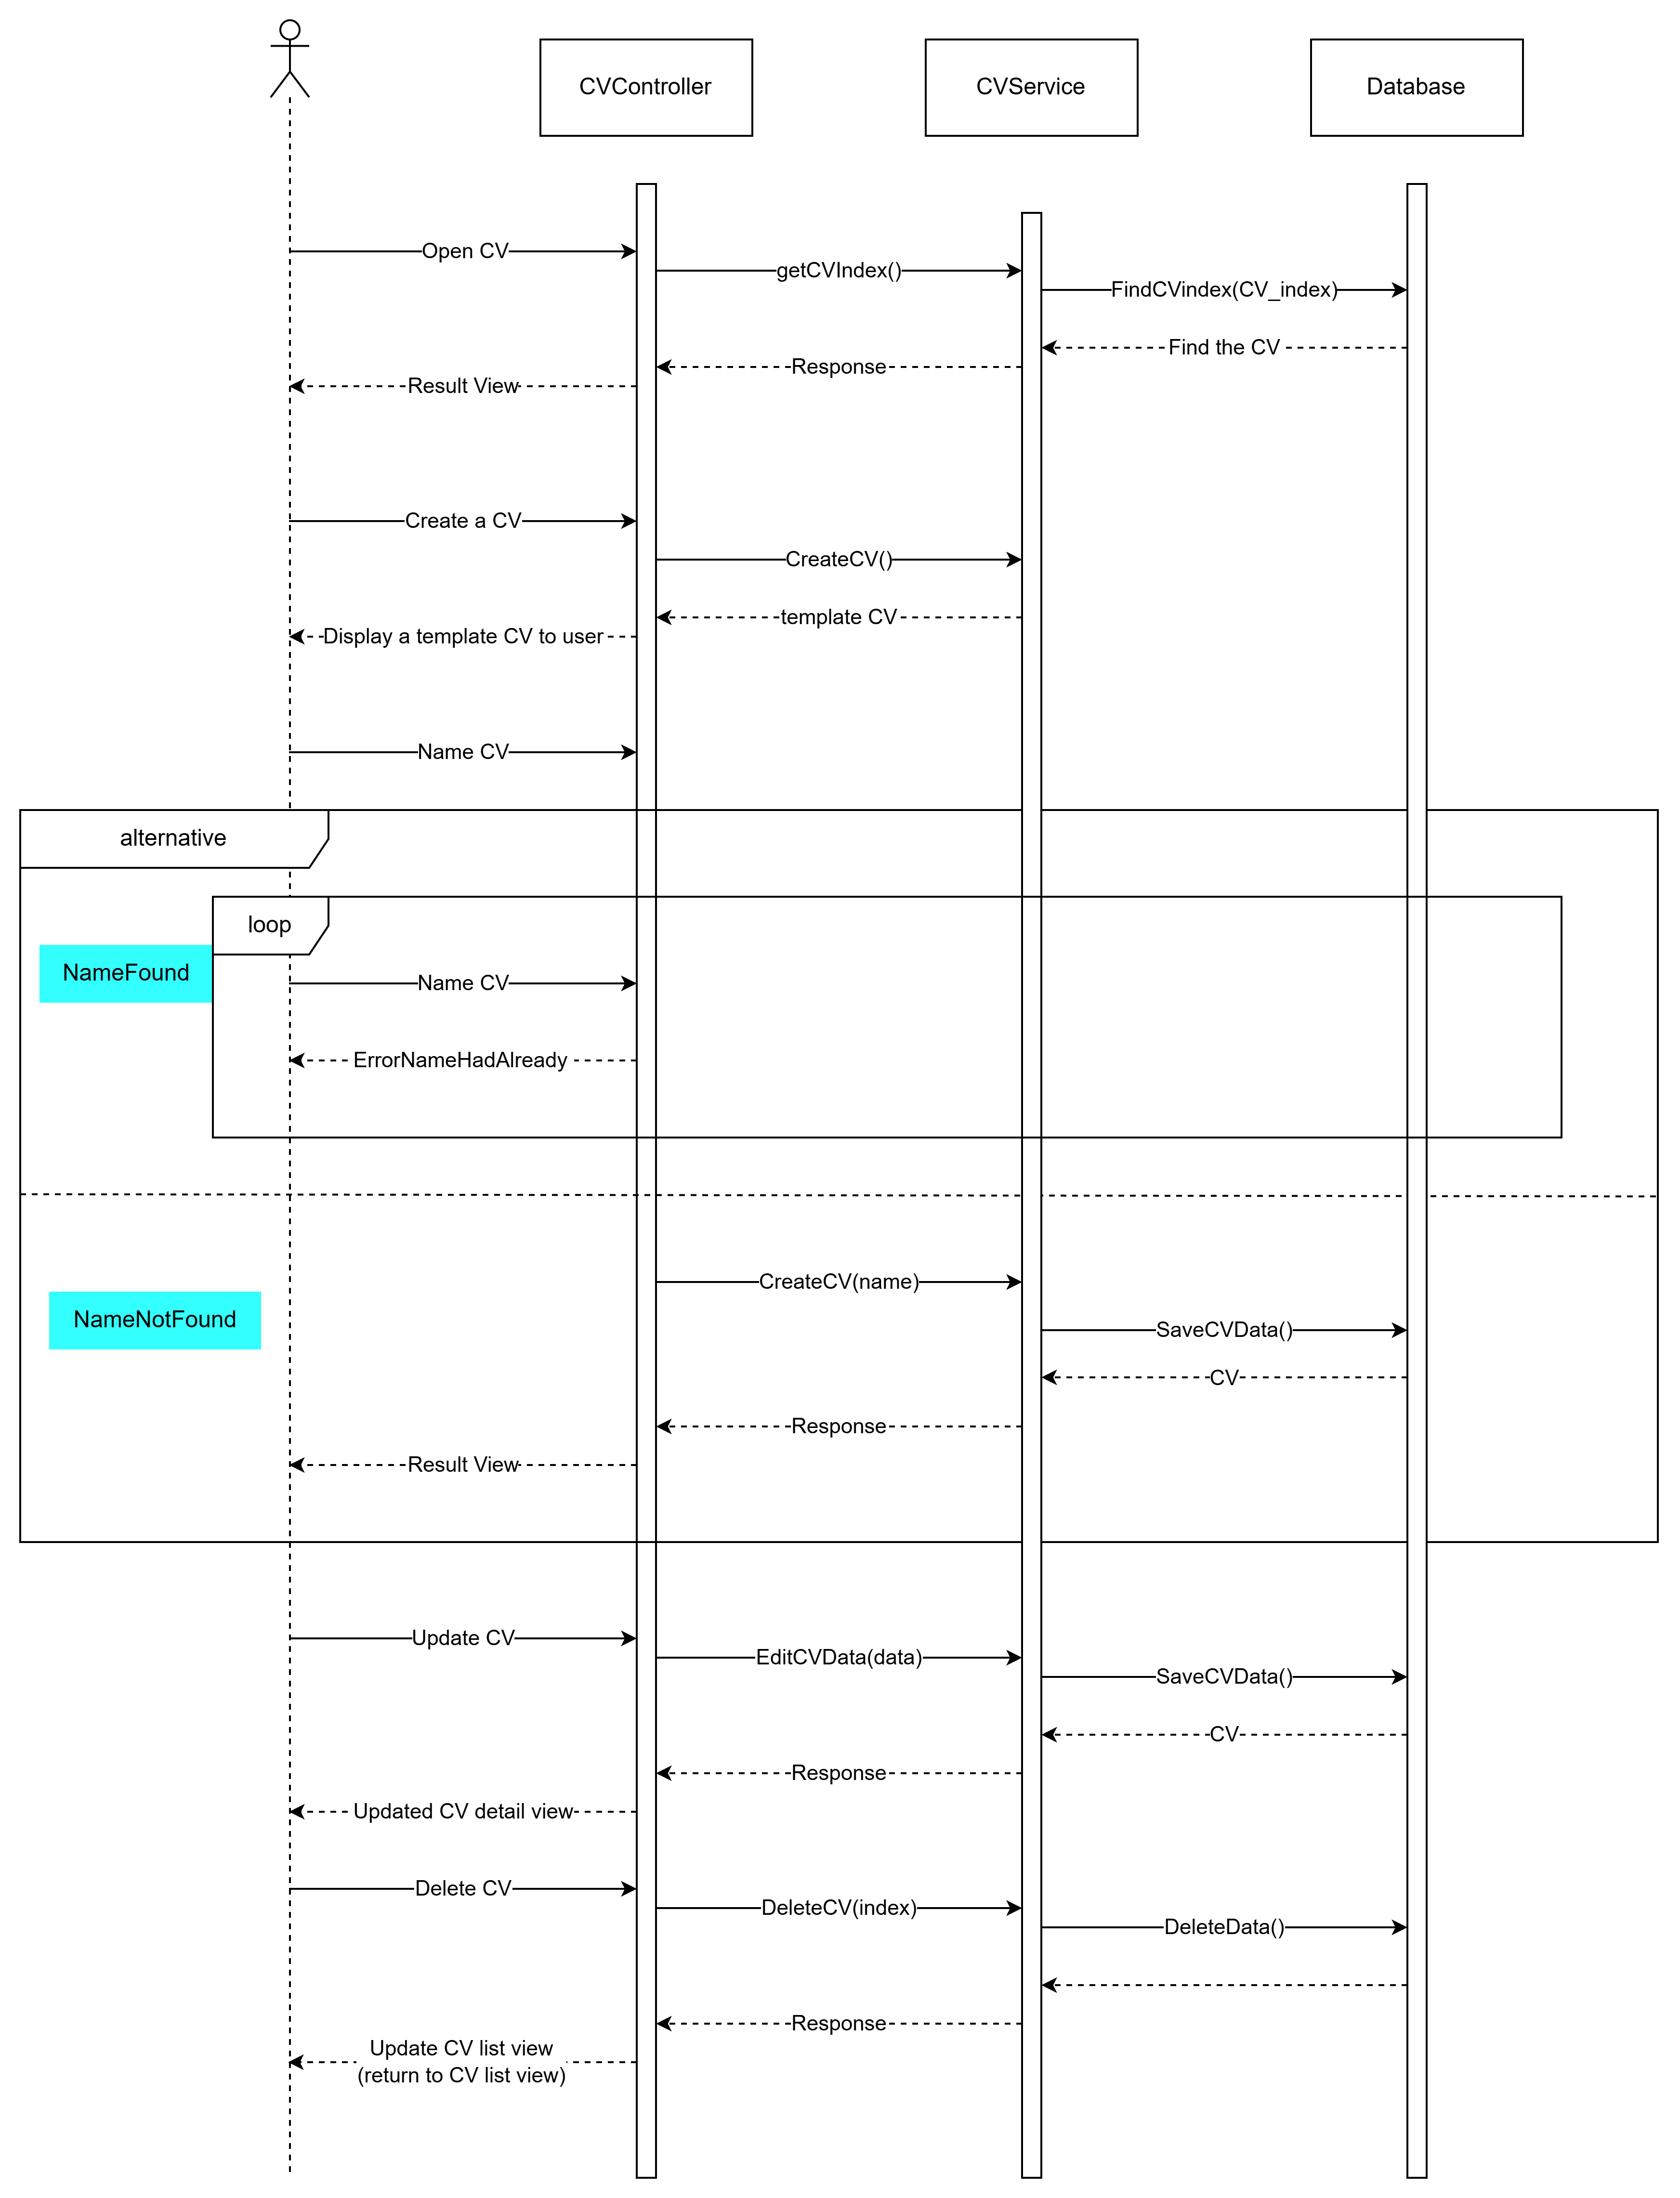
\includegraphics[scale = 0.1]{img/CV_Management_sequenceDiagram.png}
    \caption{Lược đồ tuần tự cho Quản lý CV}
	
\end{figure}

Khi người dùng vào trang "Quản lý CV", hệ thống sẽ lấy danh sách những bản CV mà người dùng đã tạo trước đó và hiển thị lên trang web. Người dùng có thể chọn chức năng "Tạo CV" để tạo thêm CV cho chính mình. Khi đó, hệ thống sẽ hiển thị một bản CV mẫu lên trang web, nhưng bản CV đó chỉ là bản nháp và nếu người dùng không lưu hay đặt tên cho bản CV, lúc thoát ra, hệ thống sẽ không lưu dữ liệu của bản CV nháp đó vào cơ sở dữ liệu của hệ thống. Còn khi đặt tên cho CV, hệ thống sẽ kiểm tra tên CV của bạn liệu có trùng tên với những CV khác của mình. Nếu có, hệ thống sẽ thông báo "Tên này đã được sử dụng. Vui lòng sử dụng tên khác". Ngược lại, nếu không trùng thì hệ thống sẽ thông báo "Lưu CV thành công".

Người dùng cũngcó thể  chọn một bản CV trong danh sách và chọn thực hiện xoá hoặc sửa CV, hệ thống sẽ lấy ID của CV vừa chọn và lấy toàn bộ thông tin của bản CV đó. Nếu người dùng chọn xoá CV, hệ thống sẽ xoá hoàn toàn dữ liệu của bản CV đó ra khỏi cơ sở dữ liệu của hệ thống. Còn nếu người dùng chọn sửa CV, hệ thống sẽ hiển thị thông tin dữ liệu của bản CV lên trang web của người dùng. Và ở đây người dùng có thể tự mình chỉnh sửa CV của mình theo ý mình muốn.


\subsection{Ứng tuyển công việc}

\begin{figure}[H]

	\centering
    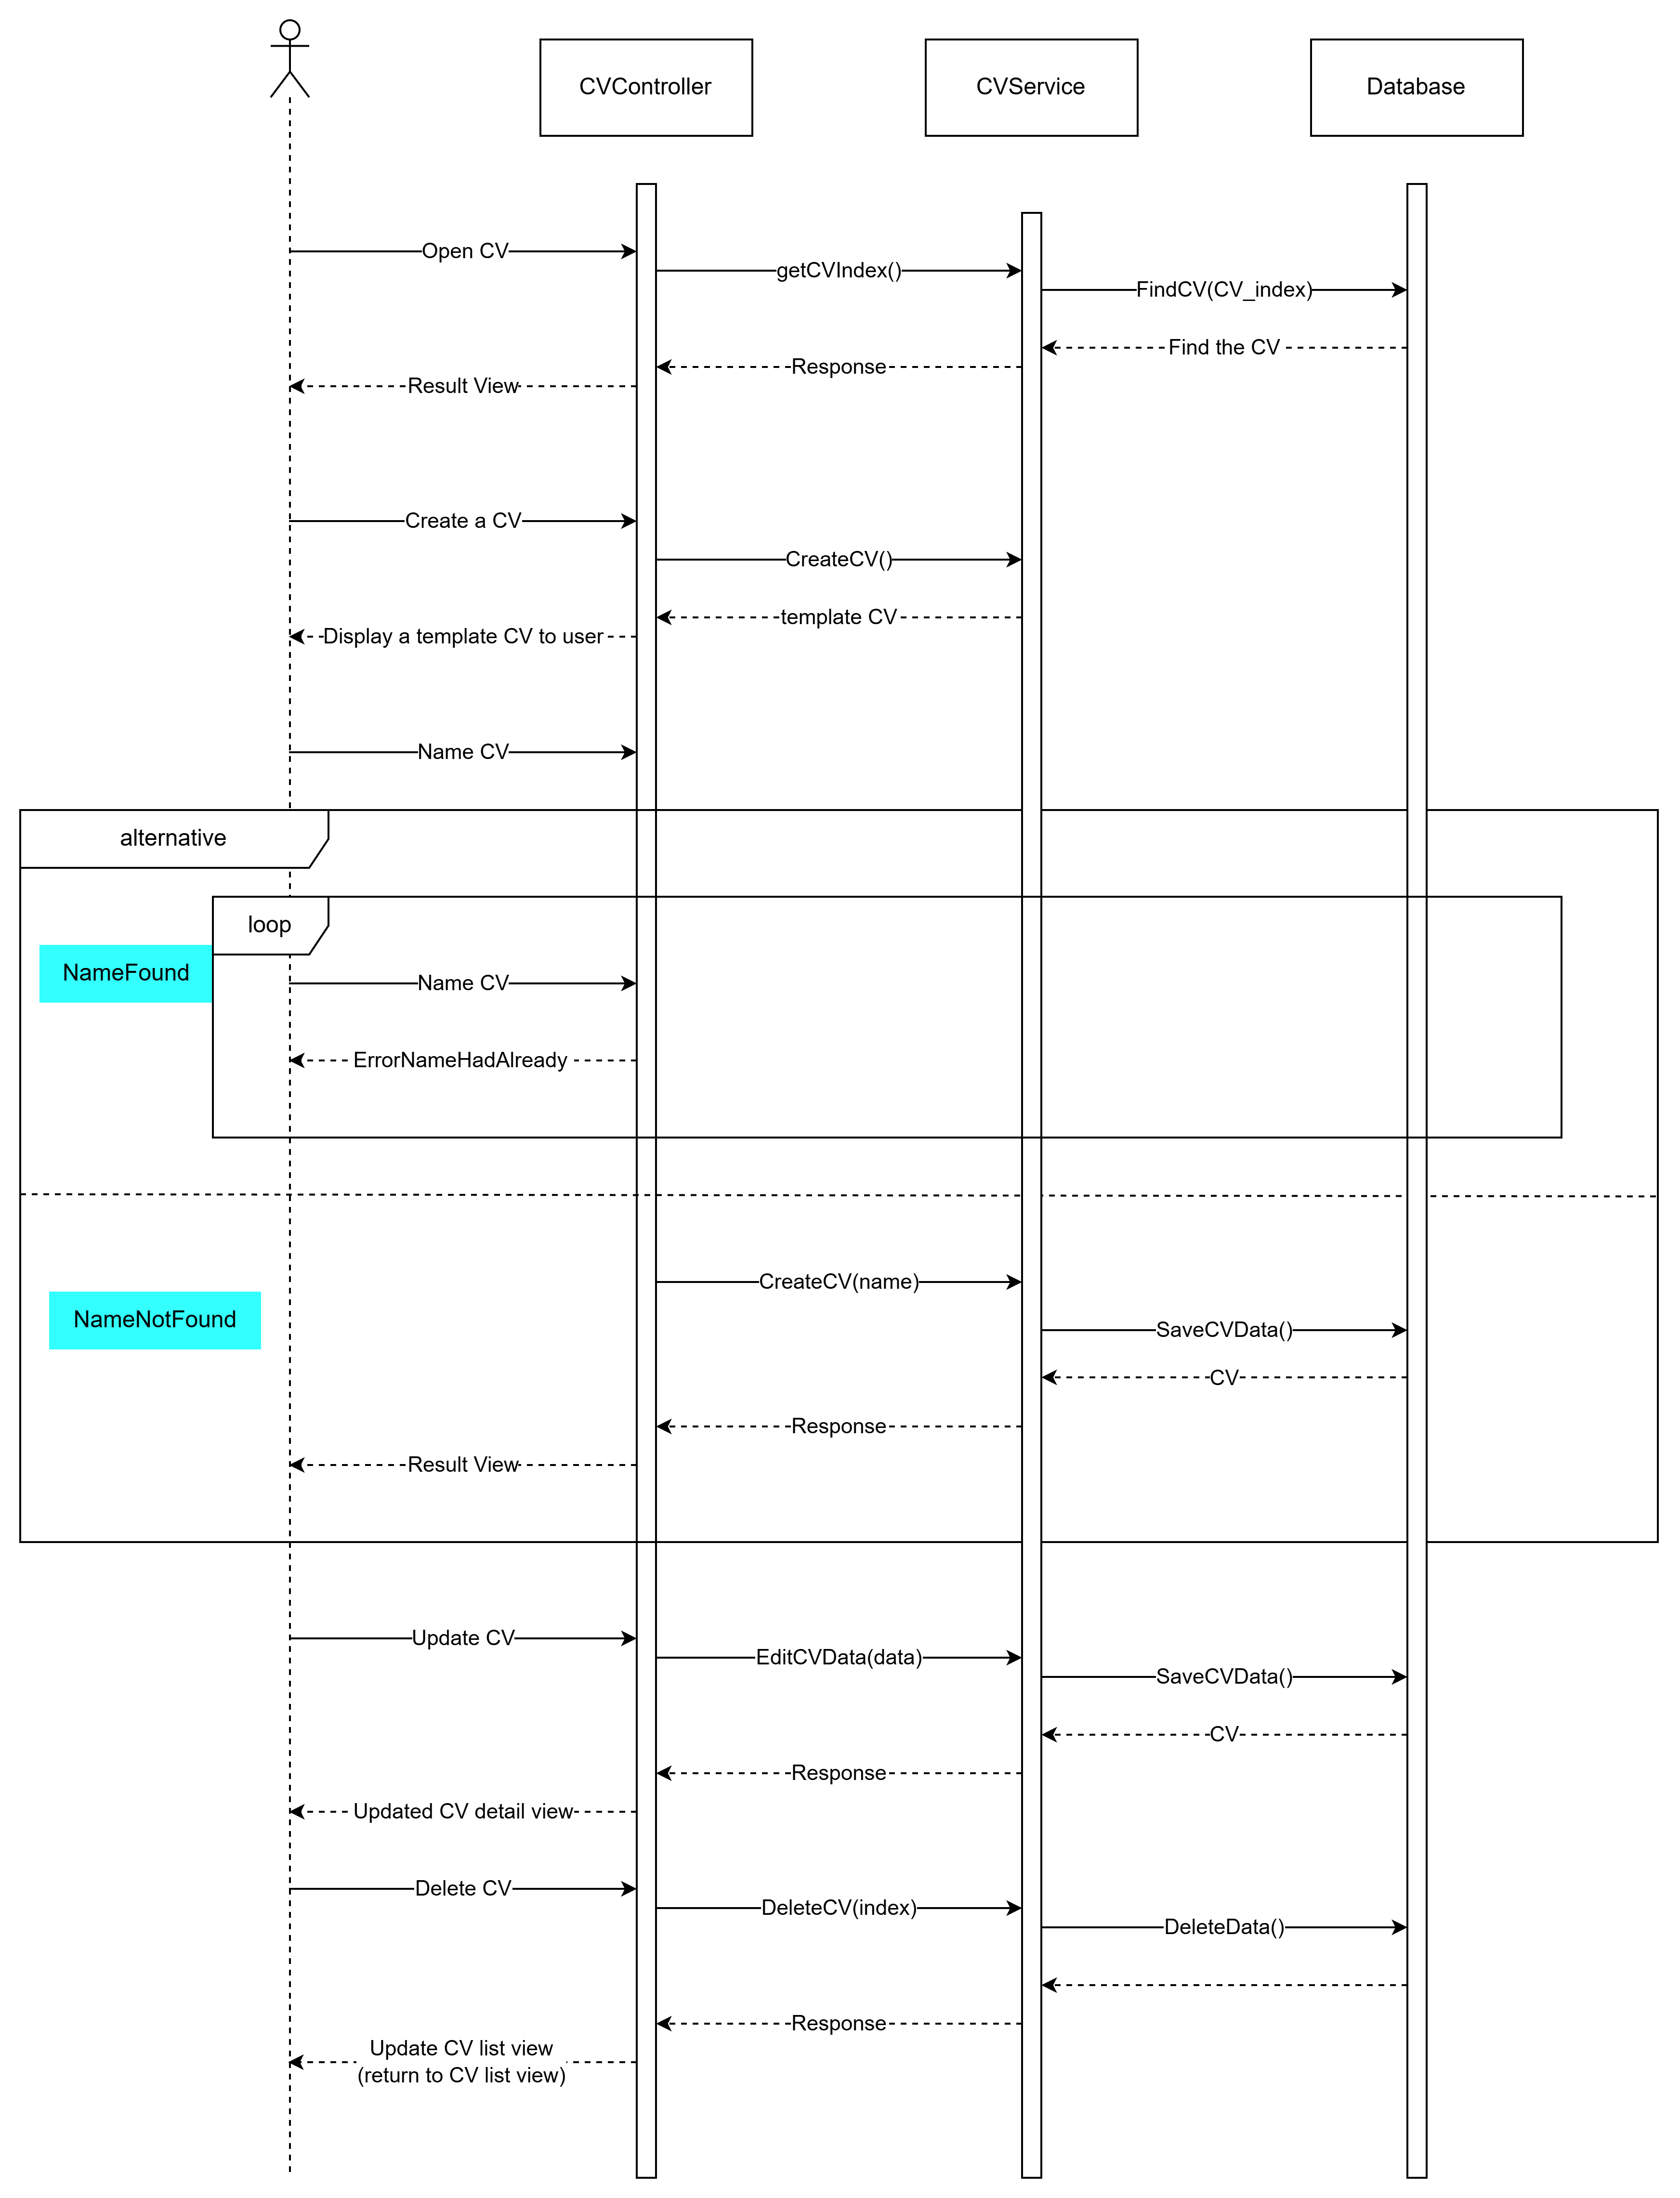
\includegraphics[scale = 0.1]{img/ApplyJob_sequenceDiagram.png}
    \caption{Lược đồ tuần tự cho Ứng tuyển công việc}
	
\end{figure}

Sơ đồ tuần tự ở trên thể hiện quy trình làm việc của một ứng viên khi ứng tuyển vào một vị trí công việc của một bài đăng tuyển dụng. Khi người dùng vào trang "Tìm kiếm việc làm", hệ thống lấy từng danh sách bài đăng tuyển dụng nhân sự và hiển thị chúng lên trang web. Mỗi bài đăng sẽ có những thông tin ngắn gọn về nội dung của bài đăng và cũng như tên công ty muốn tuyển dụng. Người dùng sẽ chọn một trong số chúng và hệ thống sẽ hiển thị toàn bộ thông tin nội dung của bài đăng.

Người sẽ đọc và nếu cảm thấy thông tin tuyển dụng thực sự phù hợp với mình, họ có thể ứng tuyển vào vị trí công việc đó của công việc. Nếu không, họ có thể chọn lựa một bài đăng khác phù hợp với tiêu chí của mình. Khi người dùng ứng tuyển vào một vị trí công việc của công ty, hệ thống sẽ kiểm tra tài khoản người dùng liệu đã có một bản CV đang trong trạng thái ứng tuyển hay chưa. Nếu chưa, hệ thống sẽ thông báo cho người dùng "Bạn vẫn chưa có CV để ứng tuyển công việc" và người dùng có thể lựa chọn hoặc ở lại trang "Tìm kiếm công việc" hoặc chuyển hướng tới trang "Quản lý CV". Sau khi chuyển hướng tới trang "Quản lý CV", người có thể tự tạo cho mình một bản CV mới hoặc có thể upload một bản CV sẵn có của mình lên trang web và đặt trạng thái CV của mình là "Ứng tuyển".

Sau cùng, người dùng sẽ được thông báo "Ứng tuyển thành công" và hệ thống sẽ gửi CV của người dùng đến công ty ứng tuyển.

\section{Thiết kế cơ sở dữ liệu}

\subsection{Thiết kế sơ đồ thực thể (ERD)}
Để thiết kế cơ sở dữ liệu, tôi đã sử dụng sơ đồ thực thể (Entity-Relationship Diagram - ERD) để trong việc thiết kế cơ sở dữ liệu để biểu diễn các thực thể trong hệ thống và mối quan hệ, tương tác giữa chúng.

\begin{figure}[H]

	\centering
    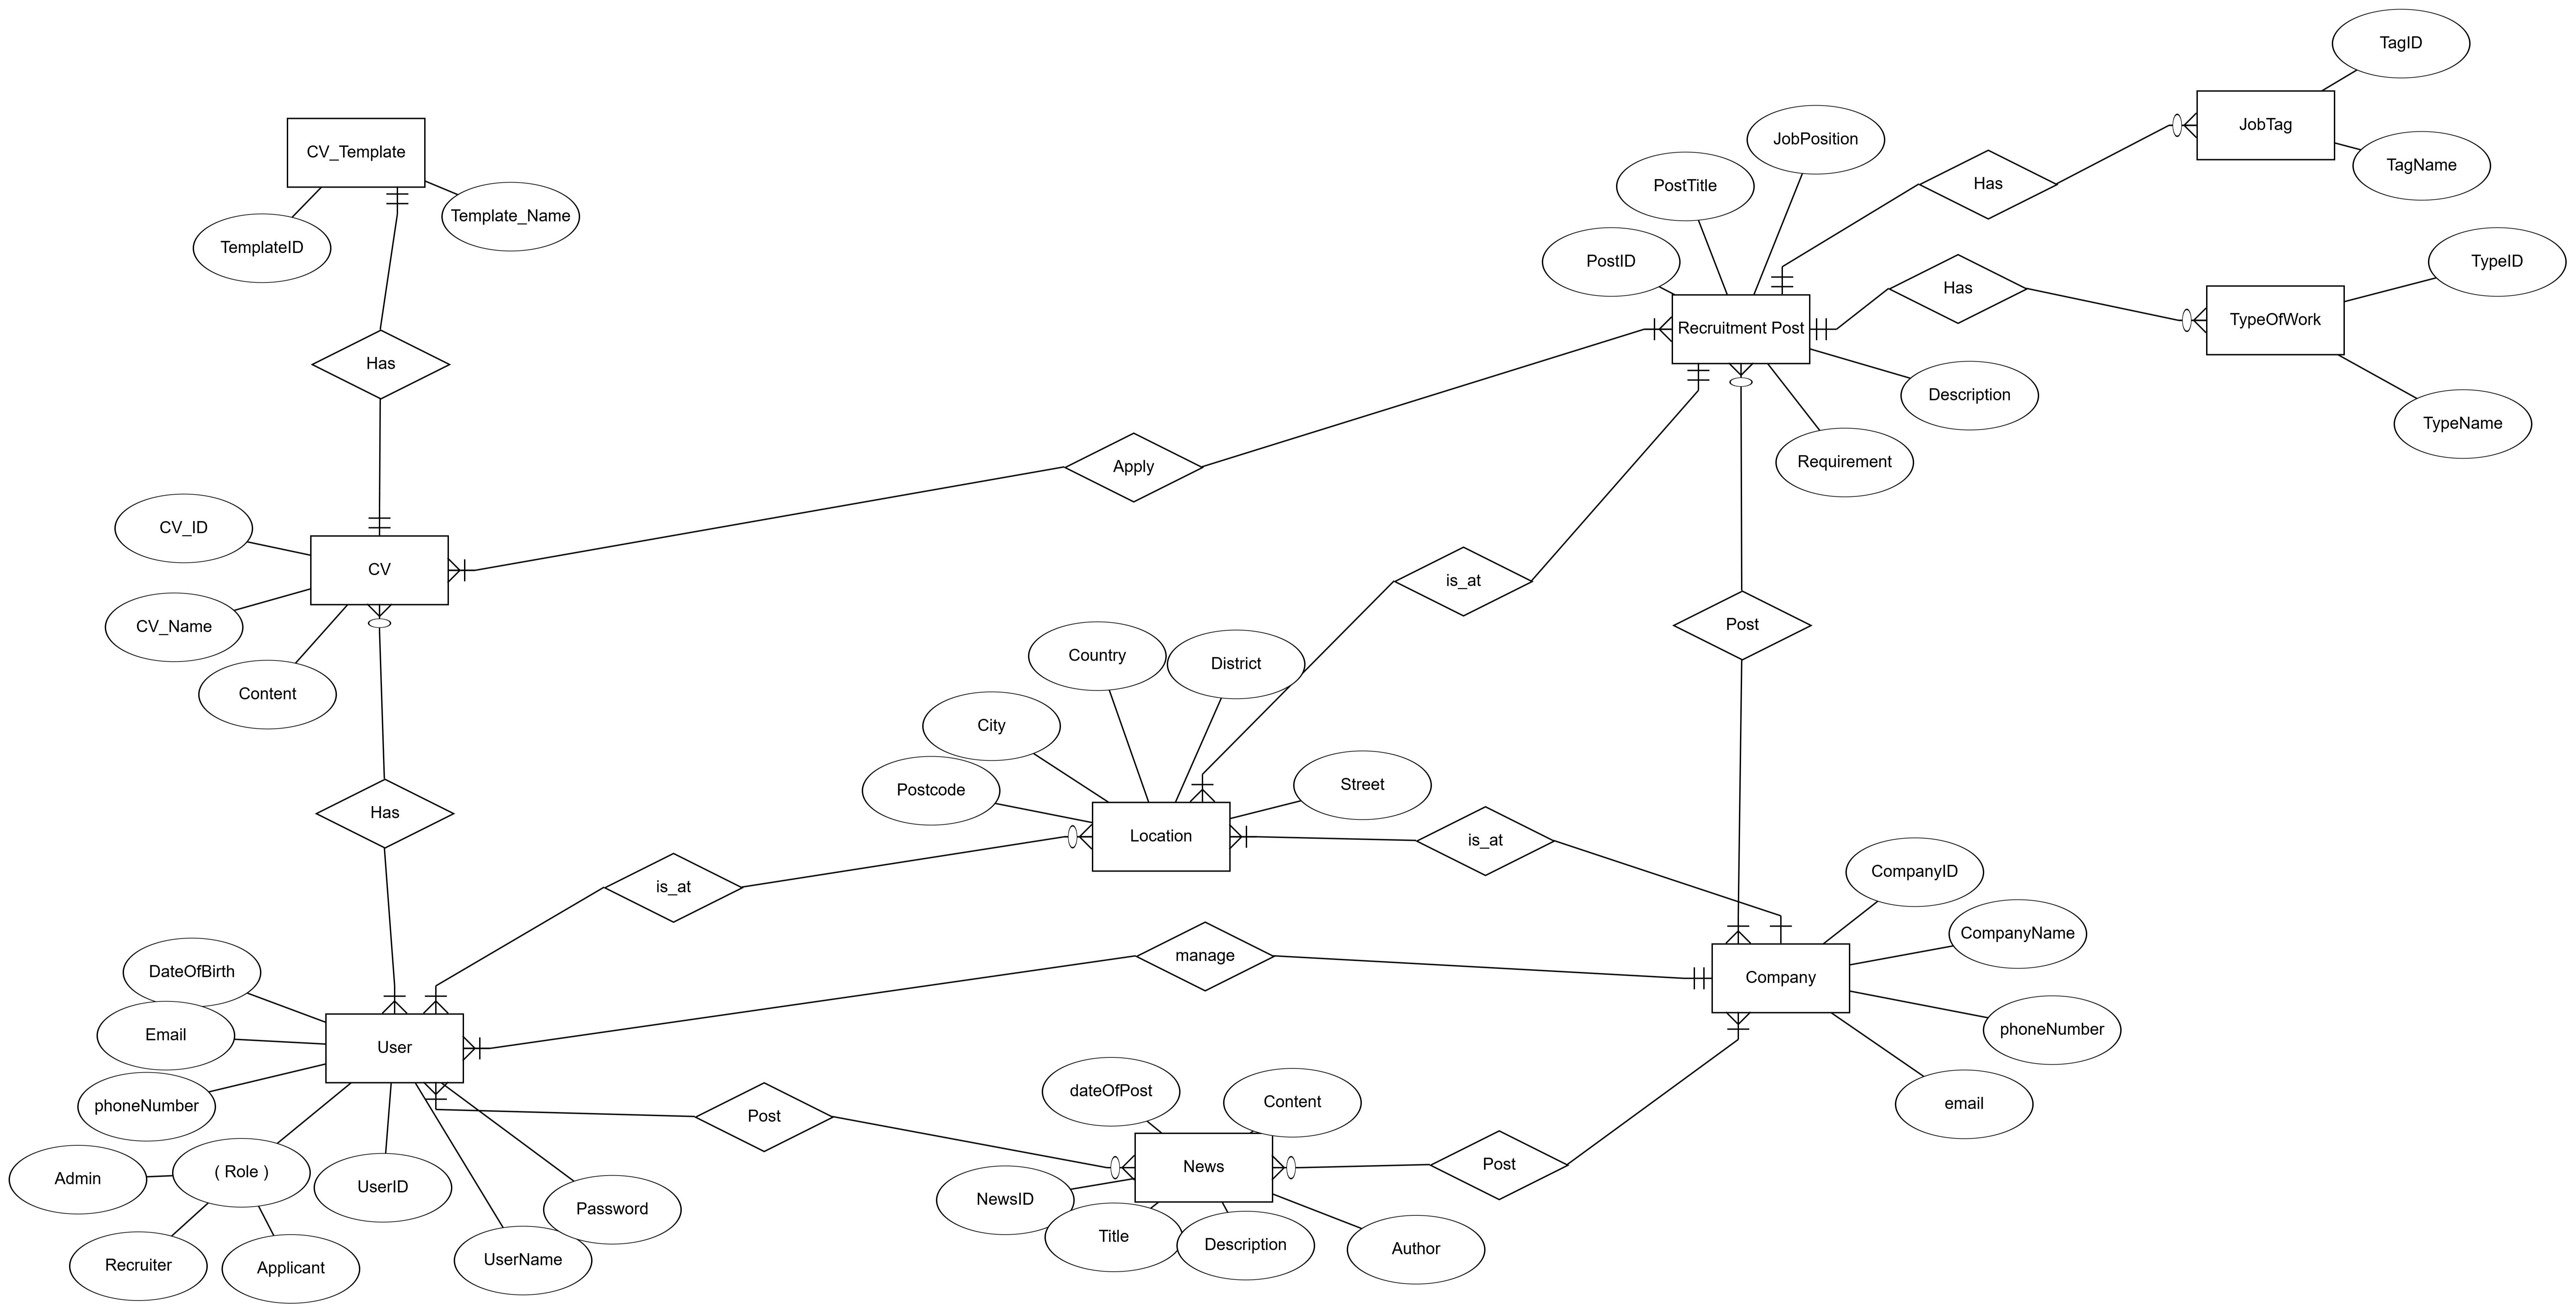
\includegraphics[angle=90,scale=0.08]{img/ERD.png}
    \caption{Sơ đồ thực thể (ERD)}
	
\end{figure}

Dưới đây là những thực thể có trong cơ sở dữ liệu của tôi:

\begin{itemize}
    \item \textbf{User:} đại diện cho các kiểu người dùng trên trang web. Nó chứa các thông tin cơ bản của người dùng và có thể thực hiện các chức năng của trang web.
    \item \textbf{Role:} đại diện cho các vai trò của người, gồm 3 role chính là: admin, applicant, recruiter/company.  Nó có thể thực hiện các chức năng cơ bản của người dùng chung. Tuy nhiên, đối với những vai trò đặc biệt như admin hay company, họ sẽ có các chức năng đặc biệt khác. VD: Đối với admin, họ có chức năng ban những users khác hay kiểm duyệt các bài đăng lên trang web,.... Hay với những doanh nghiệp (company) họ có thể thực hiện đăng những bài đăng tuyển dụng nhân viên lên trang web.
    \item \textbf{News:} là nơi chứa những thông tin, nội dung của những bản tin có trên trang web. Nó được viết và đăng lên bởi bất kỳ người dùng nào. Nhưng để được lên trang web thì cần phải được admin của trang web xét duyệt.
    \item \textbf{Recruitment Post:} là nơi chứa những thông tin, nội dung của những bài đăng tuyển dụng nhân sự của các công ty, doanh nghiệp. Nó đăng được đăng bởi doanh nghiệp, công ty. Nhưng cũng giống như tin tức (news), để lên được trang web, cần phải thông qua sự xét duyệt của admin.
    \item \textbf{CV:} là danh sách các bản CV của người dùng. Nó bao gồm: nội dung, tiêu đề, .... Mỗi CV đều có một template cho riêng mình. Tuy nhiên cũng có một bản CV custom không thuộc bất kỳ một template nào cả. Và nếu upload 1 bản CV lên trang web, hệ thông sẽ xem bản CV dưới dạng dữ liệu là file và không thể chỉnh sửa được.
    \item \textbf{CV Template:} gồm nhiều mẫu CV khác nhau phù hợp nhiều chủ đề và ngành nghề khác nhau.
    \item \textbf{Location:} đại diện cho địa chỉ của người và công ty. Đối với công ty, sẽ có nhiều địa chỉ khác nhau như: địa chỉ cơ sở chính, chi nhánh,....
    \item \textbf{Job Tag:} bao gồm các đối tượng ngành nghề mà doanh nghiệp muốn hướng đến. VD như: marketing, IT, phục vụ,... 
    \item \textbf{Type of work:} bao gồm các thể loại công việc. Nó thể hiện loại công việc, kinh nghiệm, vị trí mà công ty muốn tuyển dụng như part-time, full-time, night-shift, intern, fresher, senior,....
\end{itemize}


\subsection{Lược đồ quan hệ (Relational Schema) }

\begin{figure}[H]

	\centering
    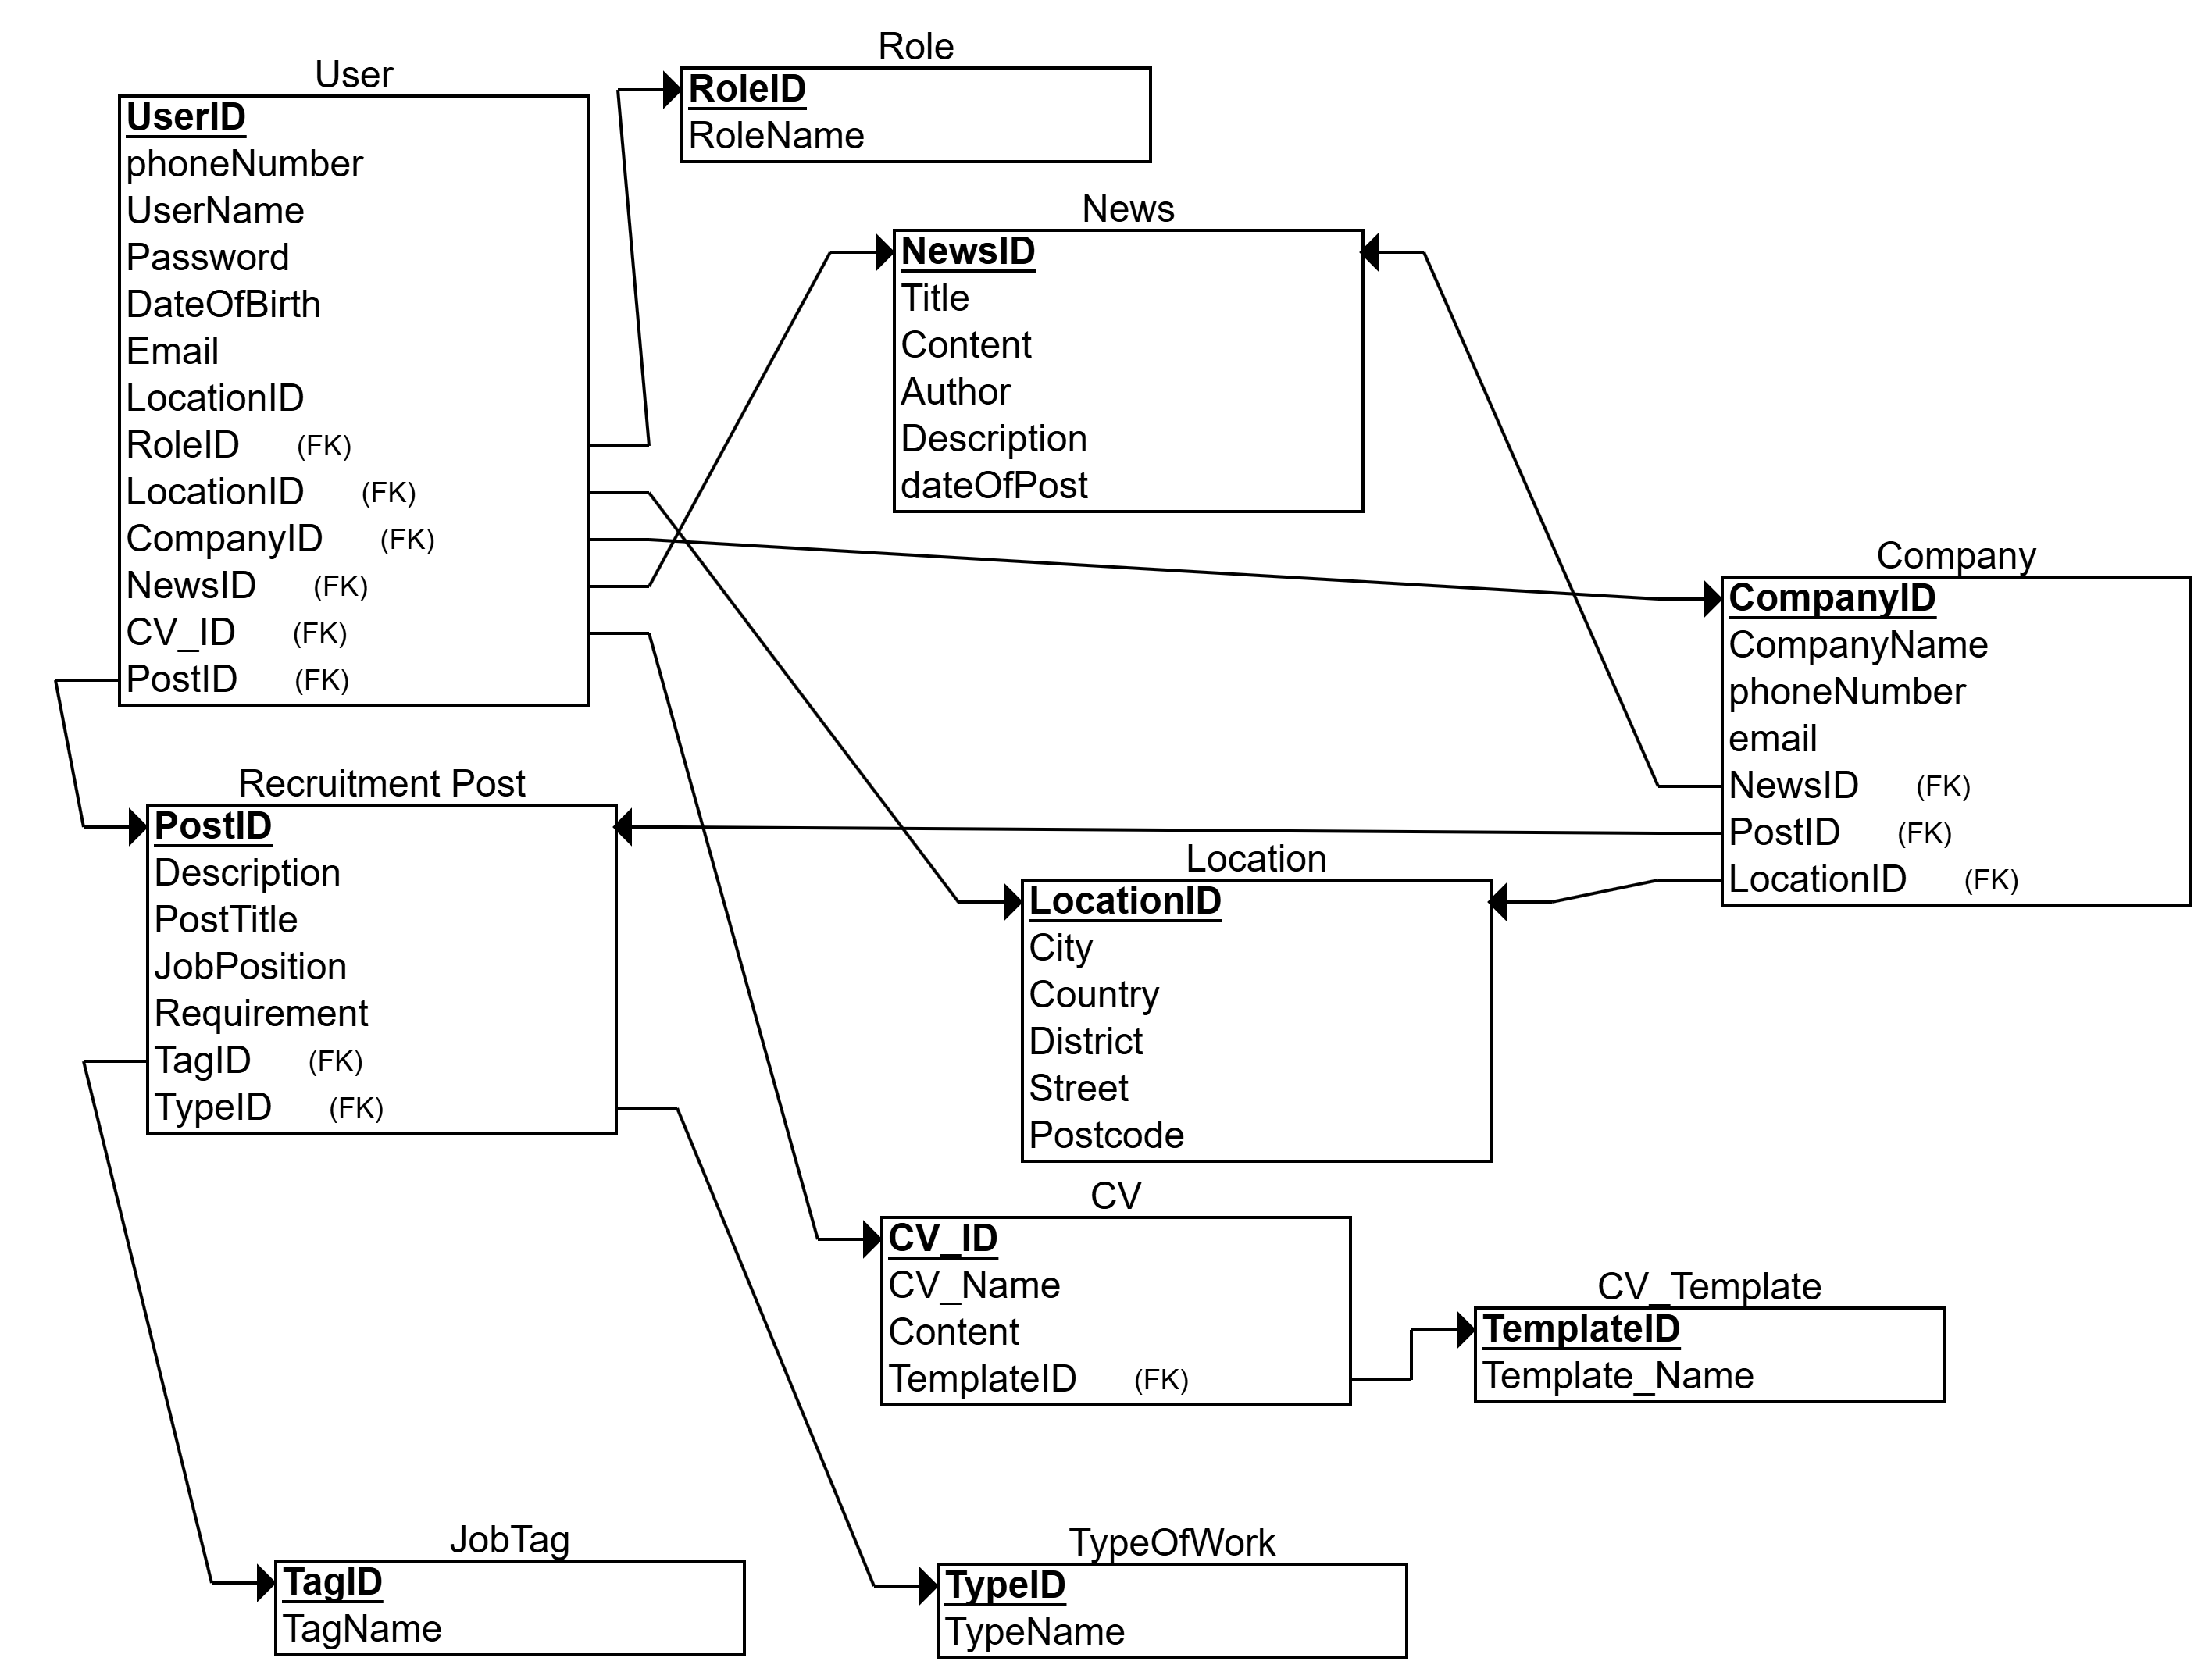
\includegraphics[scale=0.1]{img/Relational_Schema.png}
    \caption{Lược đồ quan hệ}
		
\end{figure}

